\documentclass[UTF8,a4paper,oneside]{book}
\usepackage{ctex}
\usepackage{framed}
\usepackage{amsthm}
\usepackage{geometry}
\usepackage{mathrsfs}
\geometry{left=1.414cm,right=1.314cm,top=2.414cm,bottom=2.315cm}
\usepackage{amsmath}
\usepackage{graphicx}
\usepackage{subfiles}
\linespread{1.5}
\usepackage{indentfirst}
\setlength{\parindent}{2em}

\setCJKmainfont[ItalicFont=FandolKai-Regular,BoldFont=STSongti-SC-Black]{STSong} 
\setCJKsansfont{FandolHei-Regular}
\setCJKmonofont{FandolFang-Regular}
\setCJKfamilyfont{kaiti}{FandolKai-Regular}
\setCJKfamilyfont{fang}{FandolFang-Regular}
\newcommand{\kaiti}{\CJKfamily{kaiti}}%\
\newcommand{\fang}{\CJKfamily{fang}}%
\setmainfont{Times New Roman}

%\usepackage{fourier}

\usepackage{physics}
\usepackage{paralist}

\usepackage{multicol}
\let\itemize\compactitem
\let\enditemize\endcompactitem
\let\enumerate\compactenum
\let\endenumerate\endcompactenum
\let\description\compactdesc
\let\enddescription\endcompactdesc
\usepackage{color}
\usepackage{fancyhdr} %调用宏包


\usepackage{multirow,float}
\usepackage[table]{xcolor}
%\usepackage{subfigure}
%\usepackage{hyperref}


% ---基本设置---

%设定页面的页眉页脚类型,$\LaTeX$内置了四种:empty、plain、headings及myheadings
\pagestyle{fancy}

%清除原页眉页脚样式
\fancyhf{} 

%R:页面右边;O:奇数页;\leftmark:表示“一级标题”
\fancyhead[CO]{\leftmark}

%L:页面左边;E:偶数页;\rightmark:表示“二级标题”
\fancyhead[CE]{\rightmark}

%C:页面中间
\fancyhead[CO, CE]{{\calligra The Homework For Chemical Engineering Thermodynamics}}

% 设置页脚,页眉的位置上也可以放置页码
\fancyhead[RO, LE]{$\cdot\ \textrm{\thepage} \ \cdot$}

% 设置页眉页脚横线及样式
%页眉线宽,设为0可以去页眉线
\renewcommand{\headrulewidth}{0.05em} 

%------------------------------设置字体大小------------------------%  
\newcommand{\chuhao}{\fontsize{42pt}{\baselineskip}\selectfont}     %初号  
\newcommand{\xiaochuhao}{\fontsize{36pt}{\baselineskip}\selectfont} %小初号  
\newcommand{\yihao}{\fontsize{28pt}{\baselineskip}\selectfont}      %一号  
\newcommand{\erhao}{\fontsize{21pt}{\baselineskip}\selectfont}      %二号  
\newcommand{\xiaoerhao}{\fontsize{18pt}{\baselineskip}\selectfont}  %小二号  
\newcommand{\sanhao}{\fontsize{15.75pt}{\baselineskip}\selectfont}  %三号  
\newcommand{\sihao}{\fontsize{14pt}{\baselineskip}\selectfont}       %四号  
\newcommand{\xiaosihao}{\fontsize{12pt}{\baselineskip}\selectfont}  %小四号  
\newcommand{\wuhao}{\fontsize{10.5pt}{\baselineskip}\selectfont}    %五号  
\newcommand{\xiaowuhao}{\fontsize{9pt}{\baselineskip}\selectfont}   %小五号  
\newcommand{\liuhao}{\fontsize{7.875pt}{\baselineskip}\selectfont}  %六号  
\newcommand{\qihao}{\fontsize{5.25pt}{\baselineskip}\selectfont}    %七号

\title{\textbf{《化工热力学》作业}}
\author{张博涵\quad 应化1903班\quad 学号:1912020312\\
{\calligra GitHub $:$ \href{www.github.com/BHanZhang}{www.github.com/BHanZhang}}\\
{\kaiti{起著重庄赤奋若,同年终,凡叁月。}}}
\date{}
\usepackage{chemfig}
\usepackage{mathrsfs}
\usepackage{listings}
\usepackage{makeidx}
\makeindex
\usepackage{framed}
\usepackage{amsthm,amsmath,amssymb}
\usepackage{wrapfig}
\usepackage{graphicx}
\usepackage{mathrsfs}
\bibliographystyle{plain}
\usepackage{subfiles}
\usepackage{booktabs}
\usepackage{graphicx,times}
\usepackage{esint}
\usepackage{subfigure}         
\usepackage{natbib}
\usepackage{amssymb,amsmath}
\usepackage{url}
\usepackage{geometry}
\usepackage{setspace}
\usepackage{subfigure}
\usepackage{booktabs}
\usepackage{array}
\usepackage{mhchem}
\usepackage{colortbl}
\usepackage{bm}
\usepackage{calligra}
\definecolor{myorgn}{rgb}{0.56,0.28,0.16}
\definecolor{myyelo}{rgb}{255,215,0}
\definecolor{mygray}{gray}{.9}
\definecolor{mypink}{rgb}{.99,.91,.95}
\definecolor{mycyan}{cmyk}{.3,0,0,0}
\definecolor{myblu}{RGB}{70,111,157}


\usepackage{environ}
\everymath{\displaystyle}  
\usepackage[breaklinks,colorlinks,linkcolor=black,citecolor=black,urlcolor=black]{hyperref}
\usepackage{tikz}



\definecolor{colora}{RGB}{210,185,152}
\definecolor{colorb}{rgb}{0.99,0.97,0.93}

\newcounter{problemname}
\setcounter{problemname}{0}
\newcounter{solutionname}
\setcounter{solutionname}{0}
\newcounter{tipname}
\setcounter{tipname}{0}
\usepackage{geometry}
\usepackage{lipsum}
\usepackage{newtxtext}
\usepackage{xcolor}
\usepackage{tcolorbox}

\tcbuselibrary{most}





% ------------------******-------------------
\newtcolorbox{ti}[2][]
{enhanced,breakable,
left=12pt,right=12pt,% 左右边距
coltitle=white, % 标题字体颜色
colbacktitle=colora, % 标题背景颜色
attach boxed title to top left={yshifttext=-1mm},
boxed title style={skin=enhancedfirst jigsaw,arc=1mm,bottom=0mm,boxrule=0mm},
boxrule=1pt, % 边框线宽
colback=colorb, % 文本框背景颜色
colframe=colora, % 框线颜色
sharp corners=northwest,
drop fuzzy shadow, % 可以选择是否设置阴影效果
title=\vspace{3mm}#2,
arc=1mm,
#1}

\newenvironment{problem}{\begin{ti}{\stepcounter{problemname}\Large\textbf{{\calligra{Question \arabic{problemname}}}}}}{\end{ti}\par}

% ------------------******-------------------

\usepackage[center]{titlesec}
\titleformat{\chapter}{\raggedright\Huge\bfseries}{\arabic{chapter}}{1em}{}
\titleformat{\section}{\raggedright\Large\bfseries}{\,\thesection\,}{1em}{}
\titleformat{\subsection}{\raggedright\large\bfseries}{\,\thesubsection\,}{1em}{}

\usepackage[strict]{changepage} 
\definecolor{formalshade}{rgb}{0.90,0.99,0.91} % 文本颜色
\definecolor{Green}{RGB}{74,124,42} % 文本框颜色
% ------------------******-------------------

% ------------------******-------------------
\newtcolorbox{answer}[2][]
{enhanced,breakable,
left=12pt,right=12pt,% 左右边距
coltitle=white, % 标题字体颜色
colbacktitle=Green, % 标题背景颜色
attach boxed title to top left={yshifttext=-1mm},
boxed title style={skin=enhancedfirst jigsaw,arc=1mm,bottom=0mm,boxrule=0mm},
boxrule=1pt, % 边框线宽
colback=formalshade, % 文本框背景颜色
colframe=Green, % 框线颜色
sharp corners=northwest,
drop fuzzy shadow, % 可以选择是否设置阴影效果
title=\vspace{3mm}#2,
arc=1mm,
#1}

% ------------------******-------------------

\newenvironment{solution}{\begin{answer}{\stepcounter{solutionname}\Large\textbf{{\calligra{Answer \arabic{solutionname}}}}}}{\end{answer}\par}




\definecolor{redshade}{rgb}{1.00,0.90,0.90}% 阴影颜色
\definecolor{LightCoral}{RGB}{204,22,58} % 文本框颜色
% ------------------******-------------------
\newtcolorbox{tpp}[2][]
{enhanced,breakable,
left=12pt,right=12pt,% 左右边距
coltitle=white, % 标题字体颜色
colbacktitle=LightCoral, % 标题背景颜色
attach boxed title to top left={yshifttext=-1mm},
boxed title style={skin=enhancedfirst jigsaw,arc=1mm,bottom=0mm,boxrule=0mm},
boxrule=1pt, % 边框线宽
colback=redshade, % 文本框背景颜色
colframe=LightCoral, % 框线颜色
sharp corners=northwest,
drop fuzzy shadow, % 可以选择是否设置阴影效果
title=\vspace{3mm}#2,
arc=1mm,
#1}

\newenvironment{tip}{\begin{tpp}{\stepcounter{tipname}\Large\textbf{{\calligra{Tip \arabic{tipname}}}}}}{\end{tpp}\par}

% ------------------******-------------------



\newenvironment{figurehere} 
    {\def\@captype{figure}} 
    {} 
\makeatother%用于连接公式编号


\newenvironment{tablehere} 
    {\def\@captype{table}} 
    {} 
\makeatother%用于连接公式编号

 




\newcommand{\qd}[2]{\dfrac{{\rm{d}}#1}{{\rm{d}}#2}}
\newcommand{\pd}[2]{\dfrac{\partial #1}{\partial #2}}
\newcommand{\rpd}[3]{\pqty{\dfrac{\partial #1}{\partial #2}}_{#3}}
\newcommand{\wei}[1]{{\rm{d}}#1}
\newcommand\ssd{$^{\circ}\rm{C}$}
\newcommand\sssd{^{\circ}\rm{C}}
\newcommand{\hdw}{\ce{kJ}\cdot\ce{kg}^{-1}}
\newcommand{\sdw}{\ce{kJ}\cdot\ce{kg}^{-1}\cdot\ce{K}^{-1}}


\definecolor{mygray}{gray}{.9}
\definecolor{mypink}{rgb}{.99,.91,.95}
\definecolor{mycyan}{cmyk}{.3,0,0,0}
\usepackage{environ}
\everymath{\displaystyle}  
\usepackage{tikz}


\begin{document}
\setmainfont{Times New Roman}
	\maketitle
	\tableofcontents
\chapter{2022年3月10日\quad 晴}
本次作业中的所有体积$V$均表示摩尔体积$V_{\rm{m}}$
\begin{problem}
	将下列纯物质经历的过程表示在$p-V$图上:
\begin{enumerate}
	\item 过热蒸汽等温冷凝为过冷液体
	\item 过冷液体等压加热成过热蒸汽
	\item 饱和蒸汽可逆绝热膨胀
	\item 饱和液体恒容加热
	\item 在临界点进行的恒温膨胀
\end{enumerate}
\end{problem}

\begin{solution}


\begin{wrapfigure}[8]{r}{17em} 

\vspace{-0.9cm}
	\begin{center}
\tikzset{every picture/.style={line width=0.75pt}} %set default line width to 0.75pt        

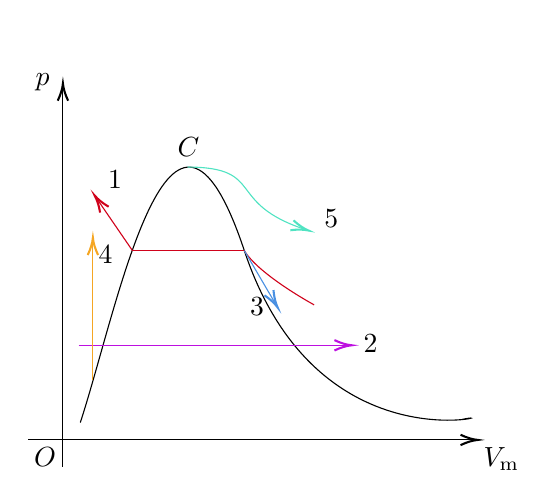
\begin{tikzpicture}[x=0.75pt,y=0.75pt,yscale=-1,xscale=1,scale=0.76]
%uncomment if require: \path (0,268); %set diagram left start at 0, and has height of 268

%Straight Lines [id:da9261157069712649] 
\draw    (33,258) -- (33,17) ;
\draw [shift={(33,15)}, rotate = 90] [color={rgb, 255:red, 0; green, 0; blue, 0 }  ][line width=0.75]    (10.93,-3.29) .. controls (6.95,-1.4) and (3.31,-0.3) .. (0,0) .. controls (3.31,0.3) and (6.95,1.4) .. (10.93,3.29)   ;
%Straight Lines [id:da40223898000413905] 
\draw    (11,241) -- (294,241) ;
\draw [shift={(296,241)}, rotate = 180] [color={rgb, 255:red, 0; green, 0; blue, 0 }  ][line width=0.75]    (10.93,-3.29) .. controls (6.95,-1.4) and (3.31,-0.3) .. (0,0) .. controls (3.31,0.3) and (6.95,1.4) .. (10.93,3.29)   ;
%Curve Lines [id:da8517089812043679] 
\draw    (44,230) .. controls (68,157) and (101,-20) .. (148,121) .. controls (195,262) and (320,221) .. (286,228) ;
%Straight Lines [id:da67833771454015] 
\draw [color={rgb, 255:red, 208; green, 2; blue, 27 }  ,draw opacity=1 ]   (77.09,121) -- (148,121) ;
%Curve Lines [id:da6846526882075424] 
\draw [color={rgb, 255:red, 208; green, 2; blue, 27 }  ,draw opacity=1 ]   (148,121) .. controls (157.25,136.37) and (192.25,155.37) .. (192.25,155.37) ;
%Straight Lines [id:da5556624828381672] 
\draw [color={rgb, 255:red, 208; green, 2; blue, 27 }  ,draw opacity=1 ]   (77.09,121) -- (54.22,87.65) ;
\draw [shift={(53.09,86)}, rotate = 55.56] [color={rgb, 255:red, 208; green, 2; blue, 27 }  ,draw opacity=1 ][line width=0.75]    (10.93,-3.29) .. controls (6.95,-1.4) and (3.31,-0.3) .. (0,0) .. controls (3.31,0.3) and (6.95,1.4) .. (10.93,3.29)   ;
%Straight Lines [id:da21149857233074754] 
\draw [color={rgb, 255:red, 189; green, 16; blue, 224 }  ,draw opacity=1 ]   (43,181) -- (214.06,181) ;
\draw [shift={(216.06,181)}, rotate = 180] [color={rgb, 255:red, 189; green, 16; blue, 224 }  ,draw opacity=1 ][line width=0.75]    (10.93,-3.29) .. controls (6.95,-1.4) and (3.31,-0.3) .. (0,0) .. controls (3.31,0.3) and (6.95,1.4) .. (10.93,3.29)   ;
%Straight Lines [id:da9678508805332595] 
\draw [color={rgb, 255:red, 74; green, 144; blue, 226 }  ,draw opacity=1 ]   (148,121) -- (168.15,155.38) ;
\draw [shift={(169.16,157.1)}, rotate = 239.63] [color={rgb, 255:red, 74; green, 144; blue, 226 }  ,draw opacity=1 ][line width=0.75]    (10.93,-3.29) .. controls (6.95,-1.4) and (3.31,-0.3) .. (0,0) .. controls (3.31,0.3) and (6.95,1.4) .. (10.93,3.29)   ;
%Straight Lines [id:da42681060344663924] 
\draw [color={rgb, 255:red, 245; green, 166; blue, 35 }  ,draw opacity=1 ]   (52,203) -- (52,114.85) ;
\draw [shift={(52,112.85)}, rotate = 90] [color={rgb, 255:red, 245; green, 166; blue, 35 }  ,draw opacity=1 ][line width=0.75]    (10.93,-3.29) .. controls (6.95,-1.4) and (3.31,-0.3) .. (0,0) .. controls (3.31,0.3) and (6.95,1.4) .. (10.93,3.29)   ;
%Curve Lines [id:da3137222686480874] 
\draw [color={rgb, 255:red, 80; green, 227; blue, 194 }  ,draw opacity=1 ]   (112,68) .. controls (162.1,68.22) and (135.16,90.77) .. (187.01,107.71) ;
\draw [shift={(188.61,108.22)}, rotate = 197.47] [color={rgb, 255:red, 80; green, 227; blue, 194 }  ,draw opacity=1 ][line width=0.75]    (10.93,-3.29) .. controls (6.95,-1.4) and (3.31,-0.3) .. (0,0) .. controls (3.31,0.3) and (6.95,1.4) .. (10.93,3.29)   ;

% Text Node
\draw (14,7.4) node [anchor=north west][inner sep=0.75pt]    {$\mathnormal{p}$};
% Text Node
\draw (298,244.4) node [anchor=north west][inner sep=0.75pt]    {$V_{\mathrm{m}}$};
% Text Node
\draw (13,244.4) node [anchor=north west][inner sep=0.75pt]    {$O$};
% Text Node
\draw (60,68.4) node [anchor=north west][inner sep=0.75pt]    {$1$};
% Text Node
\draw (222,172.4) node [anchor=north west][inner sep=0.75pt]    {$2$};
% Text Node
\draw (150,149.4) node [anchor=north west][inner sep=0.75pt]    {$3$};
% Text Node
\draw (54,116.25) node [anchor=north west][inner sep=0.75pt]    {$4$};
% Text Node
\draw (197,93.4) node [anchor=north west][inner sep=0.75pt]    {$5$};
% Text Node
\draw (104,47.4) node [anchor=north west][inner sep=0.75pt]    {$C$};
\end{tikzpicture}
        \caption{$p-V$相图}
        \label{fig1-1}
	\end{center}
\end{wrapfigure}
此题答案如右图所示:
\begin{enumerate}
	\item 右侧为过热蒸汽区,左侧为过冷液体区,在冷凝过程中等温变化(1)。
	\item 左侧为过冷液体区,右侧为过热蒸汽区,等压加热,即压力不变(2)。
	\item 饱和蒸汽可逆绝热膨胀,此时$TV^{\gamma-1} = const.$,其中$\gamma = \dfrac{C_{p}}{C_{V}}$为绝热指数。很明显由于膨胀导致的$\Delta V >0$,使得$\Delta T<0$,从而温度下降(3)。
	\item 饱和液体恒容加热,从$p-V$相图上恒容,即竖直向上(4)。
	\item 在临界点进行的恒温膨胀,即沿$T = T_{c}$线进行膨胀(5)。
\end{enumerate}
\end{solution}

\begin{problem}

	在4L的刚性容器中装有50$^{\circ}\rm{C}$、2kg水的饱和气液混合物,已知50$^{\circ}\rm{C}$时水的饱和液相体积$V^{sl}=1.0121\rm{cm}^{3}\cdot \rm{g}^{-1}$,饱和气相体积$V^{sv}=12032\rm{cm}^{3}\cdot\rm{g}^{-1}$。现在将水慢慢加热,使得饱和气液混合物变成了单相,问此单相是什么?如果将容器换为400L,最终答案是什么?
\end{problem}

\begin{solution}
\begin{enumerate}
	\item 因为是刚性容器,所以加热过程为等容变化,因此随着温度增高,压力也会增高,在$p-V$相图上相点向上移动,一直达到泡点线,相变为单液相;继续加热,相点继续向上移动,达到超临界流体区,相变为超临界流体。
	\item 如果增大容器容积,那么该体系在$p-V$相图上相点向右移动,此时加热,相点向上移动,一直达到露点线,相变为单汽相;继续加热,相点继续向上移动,达到超临界流体区,相变为超临界流体。
\end{enumerate}
\end{solution}
\begin{problem}
	试分别用(1)Van der Walls,(2)R-K方程计算273.15K时将$\ce{CO2}$压缩到比体积为550.1cm$^{3}\cdot$mol$^{-1}$所需要的压力。实验值为3.090MPa。已知$\ce{CO2}$的临界参数和偏心因子为:$T_c$=304.2K、$p_c$=7.376MPa、$\omega$=0.225
\end{problem}
\begin{solution}
	\begin{enumerate}
		\item 使用Van der Walls Eq.先计算Van der Walls常数:
		\begin{equation*}
			a = \dfrac{27}{64}\dfrac{R^{2}T_{c}^{2}}{p_{c}} = \dfrac{27}{64}\times\dfrac{8.314^{2}\times 304.2^{2}}{7.376}\rm{Pa}\cdot \rm{m}^{6}\cdot\rm{Mmol}^{-2}=365848\rm{Pa}\cdot \rm{m}^{6}\cdot\rm{Mmol}^{-2}
		\end{equation*}
		\begin{equation*}
			b = \dfrac{RT_{c}}{8p_{c}} = \dfrac{8.314\times 304.2}{8\times 7.376}\rm{m}^{3}\cdot\rm{Mmol}^{-1}= 42.86\rm{m}^{3}\cdot\rm{Mmol}^{-1}
		\end{equation*}
		然后直接带入方程:
		\begin{equation}
			p = \dfrac{RT}{V-b}-\dfrac{a}{V^{2}} = \dfrac{8.314\cdot 273.15}{550.1-42.86}-\dfrac{365848}{550.1^{2}}\rm{Mpa}=3.268\rm{Mpa}
		\label{eq1-1}
		\end{equation}
		\item 使用R-K Eq.先计算$a$、$b$:
		\begin{equation*}
			a = 0.42748\dfrac{R^{2}T_{c}^{2.5}}{p_{c}} = 0.42748\times\dfrac{8.314^{2}\times 304.2^{2.5}}{7.376}\rm{Pa}\cdot \rm{K}^{0.5}\cdot\rm{m}^{6}\cdot\rm{Mmol}^{-2}=6465661\rm{Pa}\cdot \rm{K}^{0.5}\cdot\rm{m}^{6}\cdot\rm{Mmol}^{-2}
		\end{equation*}
		\begin{equation*}
			b = 0.08664\times\dfrac{RT_{c}}{p_{c}} = 0.08664\times\dfrac{8.314\times 304.2}{ 7.376}\rm{m}^{3}\cdot\rm{Mmol}^{-1}=29.71\rm{m}^{3}\cdot\rm{Mmol}^{-1}
		\end{equation*}
		然后直接带入方程:
		\begin{equation}
			\begin{aligned}
			p = \dfrac{RT}{V-b}-\dfrac{a}{T^{0.5}V(V+b)} &=\dfrac{8.314\cdot 273.15}{550.1-29.71}-\dfrac{6465661}{273.15^{0.5}\times 550.1(550.1+29.71)} \rm{MPa}\\&= 3.137\rm{MPa}
			\end{aligned}
			\label{eq1-2}
		\end{equation}
	\end{enumerate}
\end{solution}
\begin{problem}
	使用下述方法计算1kmol甲烷贮存在体积为0.1246$\rm{m}^{3}$、温度为50$^{\circ}\rm{C}$的容器中产生的压力:(1)理想气体方程;(2)R-K方程
\end{problem}
\begin{solution}
\begin{enumerate}
	\item 使用理想气体状态方程:
	直接带入理想气体状态方程啊:
	\begin{equation*}
		p = \dfrac{nRT}{V} = \dfrac{1\times 10^{3}\times 8.314\times(50+273.15)}{0.1246}\rm{Pa} = 21.56\rm{MPa}
	\end{equation*}
	\item 使用R-K Eq.先计算$a$、$b$,首先查得甲烷的$T_{c} = 190.6$K、$p_{c} = 4.600$MPa。
		\begin{equation*}
			a = 0.42748\dfrac{R^{2}T_{c}^{2.5}}{p_{c}} = 0.42748\times\dfrac{8.314^{2}\times  190.6^{2.5}}{4.600}\rm{Pa}\cdot \rm{K}^{0.5}\cdot\rm{m}^{6}\cdot\rm{Mmol}^{-1}=3221701\rm{Pa}\cdot \rm{K}^{0.5}\cdot\rm{m}^{6}\cdot\rm{Mmol}^{-2}
		\end{equation*}
		\begin{equation*}
			b = 0.08664\times\dfrac{RT_{c}}{p_{c}} = 0.08664\times\dfrac{8.314\times 190.6}{4.600}\rm{m}^{3}\cdot\rm{Mmol}^{-1}=29.85\rm{m}^{3}\cdot\rm{Mmol}^{-1}
		\end{equation*}
		计算摩尔体积:
		\begin{equation*}
			V = \dfrac{0.1246}{1000}\rm{m}^{3}\cdot\rm{mol}^{-1}=124.6\rm{m}^{3}\cdot\rm{Mmol}^{-1}
		\end{equation*}
		然后直接带入方程:
		\begin{equation*}
			\begin{aligned}
			p = \dfrac{RT}{V-b}-\dfrac{a}{T^{0.5}V(V+b)} &=\dfrac{8.314\cdot (273.15+50)}{124.6-29.85}-\dfrac{3221701}{(273.15+50)^{0.5}\times 124.6(124.6+29.85)}\rm{MPa}\\&= 19.04\rm{MPa}
			\end{aligned}
		\end{equation*}
\end{enumerate}
\end{solution}

\begin{problem}
	试分别用(1)Van der Walls,(2)R-K方程计算0$^{\circ}\rm{C}$时将CO$_{2}$压缩到密度为80kg$\cdot$m$^{-3}$所需要的压力,并和实验值(3.09$\times$10$^{6}$Pa)进行比较。已知CO$_{2}$的临界参数和偏心因子为:$T_c=304.2$K 、$p_{c}$=7.376MPa  、$\omega$=0.225
\end{problem}

\begin{solution}
压缩至$80\rm{kg}\cdot\rm{m}^{-3}$,此时的摩尔体积为:\begin{equation*}
	V = \dfrac{1}{\dfrac{80\times 10^{3}}{40.02}}\rm{m}^{3}\cdot\rm{mol}^{-1} = 500.1\rm{m}^{3}\cdot\rm{Mmol}^{-1}
\end{equation*}
然后和本次作业第三题一样,答案如式(\ref{eq1-1})、(\ref{eq1-2})。
\end{solution}


\begin{problem}
	试分别用(1)Van der Walls,(2)R-K方程计算1kmol甲烷在166.7K时进行等温压缩,当其终态体积为0.619$\rm{m}^{3}$时,应加的压力为多少?已知文献值为1.72MPa。
\end{problem}

\begin{solution}
查得甲烷的$T_{c} = 190.6$K、$p_{c} = 4.600$MPa。其摩尔体积为$V = 0.619\times 10^{-3}\rm{m}^{3}\cdot\rm{mol}^{-1} = 619\rm{m}^{3}\cdot\rm{Mmol}^{-1}$

	\begin{enumerate}
		\item 使用Van der Walls Eq.先计算Van der Walls常数:
		\begin{equation*}
			a = \dfrac{27}{64}\dfrac{R^{2}T_{c}^{2}}{p_{c}} = \dfrac{27}{64}\times\dfrac{8.314^{2}\times 190.6^{2}}{4.600}\rm{Pa}\cdot \rm{m}^{6}\cdot\rm{Mmol}^{-2}=230299\rm{Pa}\cdot \rm{m}^{6}\cdot\rm{Mmol}^{-2}
		\end{equation*}
		\begin{equation*}
			b = \dfrac{RT_{c}}{8p_{c}} = \dfrac{8.314\times 190.6}{8\times 4.600}\rm{m}^{3}\cdot\rm{Mmol}^{-1}= 43.06\rm{m}^{3}\cdot\rm{Mmol}^{-1}
		\end{equation*}
		然后直接带入方程:
		\begin{equation*}
			p = \dfrac{RT}{V-b}-\dfrac{a}{V^{2}} = \dfrac{8.314\cdot 166.7}{619-43.06}-\dfrac{230299}{619^{2}}\rm{Mpa}=1.805\rm{Mpa}
		\end{equation*}
		\item 使用R-K Eq.先计算$a$、$b$:
		\begin{equation*}
			a = 0.42748\dfrac{R^{2}T_{c}^{2.5}}{p_{c}} = 0.42748\times\dfrac{8.314^{2}\times 190.6^{2.5}}{4.600}\rm{Pa}\cdot \rm{K}^{0.5}\cdot\rm{m}^{6}\cdot\rm{Mmol}^{-2}=3221701\rm{Pa}\cdot \rm{K}^{0.5}\cdot\rm{m}^{6}\cdot\rm{Mmol}^{-2}
		\end{equation*}
		\begin{equation*}
			b = 0.08664\times\dfrac{RT_{c}}{p_{c}} = 0.08664\times\dfrac{8.314\times 190.6}{4.600}\rm{m}^{3}\cdot\rm{Mmol}^{-1}=29.84\rm{m}^{3}\cdot\rm{Mmol}^{-1}
		\end{equation*}
		然后直接带入方程:
		\begin{equation*}
			\begin{aligned}
			p = \dfrac{RT}{V-b}-\dfrac{a}{T^{0.5}V(V+b)} &=\dfrac{8.314\cdot 166.7}{619-29.84}-\dfrac{3221701}{166.7^{0.5}\times 619(619+29.84)} \rm{MPa}\\&= 1.731\rm{MPa}
			\end{aligned}
		\end{equation*}
	\end{enumerate}
\end{solution}
\chapter{2022年3月30日\quad 多云$^{\star}$}
\begin{problem}
	试用下列方法计算510K、2.5MPa下正丁烷的摩尔体积。已知实验值为1.4807m$^{3}\cdot$kmol$^{-1}$。(1)用理想气体方程;(2)用普遍化第二维里系数关联。已知正丁烷的临界参数:$T_{c} = 425.2$K、$p_{c} = 3.8$MPa、$\omega = 0.193$
\end{problem}
\begin{solution}
	\begin{enumerate}
		\item 直接带入计算呗:
		\begin{equation*}
			V_{m} = \dfrac{RT}{p} = \dfrac{8.314\times 510}{2.5}\rm{m}^{3}\cdot\rm{Mmol}^{-1} = 1696.0\rm{m}^{3}\cdot\rm{Mmol}^{-1}=1.6960\rm{m}^{3}\cdot\rm{kmol}^{-1}
		\end{equation*}
		\item 此时对比状态:
		\begin{equation*}
			T_{r} = \dfrac{T}{T_{c}} = \dfrac{510}{425.2}=1.198
		\end{equation*}
		\begin{equation*}
			p_{r} = \dfrac{p}{p_{c}} = \dfrac{2.5}{3.8}=0.66
		\end{equation*}
		然后根据Pitzer的关系式:
		\begin{equation*}
			B^{0} = 0.083-\dfrac{0.422}{T_{r}^{1.6}}=0.083-\dfrac{0.422}{1.198^{1.6}} = -0.233
		\end{equation*}
		\begin{equation*}
			B^{1} = 0.139-\dfrac{0.172}{T_{r}^{4.2}} = 0.139-\dfrac{0.172}{1.198^{4.2}} = 0.0555
		\end{equation*}
		对比第二Virial系数为:
		\begin{equation*}
			\widehat{B} =\dfrac{Bp_{c}}{RT_{c}}= B^{0}+\omega B^{1} = -0.233+0.193\times 0.0555=-0.222
		\end{equation*}
		压缩因子:
		\begin{equation*}
			Z = 1+\widehat{B}\cdot\dfrac{p_{r}}{T_{r}} = 1-0.222\cdot\dfrac{0.66}{1.198} = 0.877
		\end{equation*}
		既得到:
		\begin{equation*}
			V_{m} = \dfrac{ZRT}{p} = \dfrac{0.877\times 8.314\times 510}{2.5}\rm{m}^{3}\cdot\rm{Mmol}^{-1}=1487.4\rm{m}^{3}\cdot\rm{Mmol}^{-1}=1.4874\rm{m}^{3}\cdot\rm{kmol}^{-1}
		\end{equation*}
	\end{enumerate}
\end{solution}

\begin{problem}
	试计算含有30\%(摩尔分数)氮气(1)和70\%(摩尔分数)正丁烷(2)气体混合物7g,在188$^{\circ}\rm{C}$、6.888MPa条件下的体积。已知$B_{11}$=14cm$^{3}\cdot$mol$^{-1}$,$B_{22}$=$-$265cm$^{3}\cdot$mol$^{-1}$,$B_{12}$=$-$9.5cm$^{3}\cdot$mol$^{-1}$。
\end{problem}
\begin{solution}
	第二Virial系数算为:
	\begin{equation*}
		\begin{aligned}
		B = y_{1}^{2}B_{11}+2y_{1}y_{2}B_{12}+y_{2}^{2}B_{22} &= 0.3^{2}\times 14+2\times 0.3\times 0.7\times (-9.5)+0.7^{2}\times(-265)\rm{cm}^{3}\times\rm{mol}^{-1}\\
		&=-132.6\rm{cm}^{3}\times\rm{mol}^{-1}
		\end{aligned} 
	\end{equation*}
	压缩因子为:
	\begin{equation*}
		Z = 1+\dfrac{Bp}{RT} =1+ \dfrac{-132.6\times 6.88}{8.314\times(273.15+188)}=0.762
	\end{equation*}
	既得到:
		\begin{equation*}
			V_{m} = \dfrac{ZRT}{p} = \dfrac{0.762\times 8.314\times (273.15+188)}{6.888}\rm{m}^{3}\cdot\rm{Mmol}^{-1}=424.1\rm{cm}^{3}\cdot\rm{mol}^{-1}
		\end{equation*}
		又根据Amagat分体积定律可得气体混合物的物质的量为:
		\begin{equation*}
			n = \dfrac{7}{28\times 0.3+58\times 0.7} \rm{mol}= 0.1429\rm{mol}
		\end{equation*}
		则气体体积为:
		\begin{equation*}
			V = nV_{m} =424.1\times 0.1429\rm{cm}^{3} = 60.60\rm{cm}^{3}
		\end{equation*}
\end{solution}
\begin{problem}
	某企业需要等摩尔氮气(1)和甲烷(2)的混合4.5kg,为了减少运输成本,需要将该气体在等温下从0.10133MPa、$-$17.78\ssd 压缩到5.0665MPa。试用普遍化第二维里系数关系式计算压缩前后的气体体积比。(取$k_{ij} = 0$)
	\begin{itemize}
		\item 已知\ce{N2}的临界数据为:$T_{c_{1}} = 126.2$K, $p_{c_{1}}=3.394$MPa, $\omega_{1}$=0.040,$Z_{c_{1}}$=0.290, $V_{c_{1}}$=89.5cm$^{3}\cdot$mol$^{-1}$;
		\item 已知\ce{CH4}的临界数据为:$T_{c_{2}} = 190.6$K, $p_{c_{2}}=4.600$MPa, $\omega_{2}$=0.008,$Z_{c_{2}}$=0.288, $V_{c_{2}}$=99cm$^{3}\cdot$mol$^{-1}$。
	\end{itemize}
\end{problem}
	
\begin{solution}
首先要计算各对比状态:
\begin{itemize}
	\item 对比温度:$T = 273.15-17.78 \rm{K}= 255.37\rm{K}$\begin{equation*}
	T_{r_{1}} = T_{r_{\ce{N2}}} = \dfrac{T}{T_{c_{1}}} = \dfrac{255.37}{126.2}=2.023
		\end{equation*} 
		\begin{equation*}
	T_{r_{2}} = T_{r_{\ce{CH4}}} = \dfrac{T}{T_{c_{2}}} = \dfrac{255.37}{190.6}=1.340
		\end{equation*} 
	\item 对比压力:\begin{itemize}
	\item 压缩前:\begin{equation*}
		p_{r_{11}} = p_{r_{1,\ce{N2}}} = \dfrac{p_{1}}{p_{c_{1}}}=\dfrac{0.10133}{3.394} = 0.02986
	\end{equation*}
	\begin{equation*}
		p_{r_{12}} = p_{r_{1,\ce{CH4}}} = \dfrac{p_{1}}{p_{c_{2}}}=\dfrac{0.10133}{4.6} = 0.02203
	\end{equation*}
	\item 压缩后:\begin{equation*}
		p_{r_{2,\ce{N2}}} = \dfrac{p_{2}}{p_{c_{1}}}=\dfrac{5.0665}{3.394} = 1.493
	\end{equation*}
	\begin{equation*}
		p_{r_{2,\ce{CH4}}} = \dfrac{p_{2}}{p_{c_{2}}}=\dfrac{5.0665}{4.6} = 1.101
		\end{equation*}
	
\end{itemize}
\end{itemize}

	根据普遍化第二Virial系数关系式:
	\begin{itemize}
		\item 压缩前:\begin{equation*}
		\begin{aligned}
		\dfrac{V_{11}}{V_{12}} = \dfrac{V_{1,\ce{N2}}}{V_{1,\ce{CH4}}} &=\dfrac{1+\left[\left(0.083+\dfrac{0.422}{T_{r_{1}}^{1.6}}\right)+\omega_{1}\times\left(0.139-\dfrac{0.172}{T_{r_{1}}^{4.2}}\right)\right]\dfrac{p_{r_{11}}}{T_{r_{1}}}}{1+\left[\left(0.083+\dfrac{0.422}{T_{r_{1}}^{1.6}}\right)+\omega_{2}\times\left(0.139-\dfrac{0.172}{T_{r_{1}}^{4.2}}\right)\right]\dfrac{p_{r_{12}}}{T_{r_{1}}}} \\
		&=\dfrac{\left[\left(0.083+\dfrac{0.422}{T_{r_{1}}^{1.6}}\right)+\omega_{1}\times\left(0.139-\dfrac{0.172}{T_{r_{1}}^{4.2}}\right)\right]p_{r_{11}}+T_{r_{1}}}{\left[\left(0.083+\dfrac{0.422}{T_{r_{1}}^{1.6}}\right)+\omega_{2}\times\left(0.139-\dfrac{0.172}{T_{r_{1}}^{4.2}}\right)\right]p_{r_{12}}+T_{r_{1}}} \\
		&= \dfrac{\left[\left(0.083+\dfrac{0.422}{2.023^{1.6}}\right)+0.040\times\left(0.139-\dfrac{0.172}{2.023^{4.2}}\right)\right]\times 0.02986+2.023}{\left[\left(0.083+\dfrac{0.422}{2.023^{1.6}}\right)+0.008\times\left(0.139-\dfrac{0.172}{2.023^{4.2}}\right)\right]\times 0.02203+2.023}  = 1.001
		\end{aligned}
	\end{equation*}
	\item 压缩后,同理如:
\begin{equation*}
		\begin{aligned}
		\dfrac{V_{21}}{V_{22}} = \dfrac{V_{2,\ce{N2}}}{V_{2,\ce{CH4}}} &=\dfrac{\left[\left(0.083+\dfrac{0.422}{T_{r_{2}}^{1.6}}\right)+\omega_{1}\times\left(0.139-\dfrac{0.172}{T_{r_{2}}^{4.2}}\right)\right]p_{r_{21}}+T_{r_{2}}}{\left[\left(0.083+\dfrac{0.422}{T_{r_{2}}^{1.6}}\right)+\omega_{2}\times\left(0.139-\dfrac{0.172}{T_{r_{2}}^{4.2}}\right)\right]p_{r_{22}}+T_{r_{2}}} \\
		&= \dfrac{\left[\left(0.083+\dfrac{0.422}{1.340^{1.6}}\right)+0.040\times\left(0.139-\dfrac{0.172}{1.340^{4.2}}\right)\right]\times 1.493+1.340}{\left[\left(0.083+\dfrac{0.422}{1.340^{1.6}}\right)+0.008\times\left(0.139-\dfrac{0.172}{1.340^{4.2}}\right)\right]\times 1.101+1.340}  = 1.082
		\end{aligned}
\end{equation*}
% 这确实不能这么算
%	\begin{equation*}
%	\begin{aligned}
%		\dfrac{V_{21}}{V_{22}}= \dfrac{Z_{2,\ce{N2}}}{Z_{2,\ce{CH4}}}=\dfrac{Z_{r_{\ce{N2}}}Z_{c_{\ce{N2}}}}{Z_{r_{2,\ce{CH4}}}Z_{c_{\ce{CH4}}}}&=\dfrac{0.290}{0.228}\dfrac{Z_{r_{2,\ce{N2}}}}{Z_{r_{\ce{CH4}}}}\\
%		&=1.272\dfrac{Z_{r_{2,\ce{N2}}}}{Z_{r_{2,\ce{CH4}}}}=1.272\dfrac{\dfrac{p_{r_{2,\ce{CH4}}}V_{r_{2,\ce{CH4}}}}{RT_{r_{2}}}}{\dfrac{p_{r_{2,\ce{CH4}}}V_{r_{2,\ce{N2}}}}{RT_{r_{2}}}}\\
%		&=1.272\dfrac{p_{r_{2,\ce{N2}}}V_{r_{2,\ce{N2}}}}{p_{r_{2,\ce{CH4}}}V_{r_{2,\ce{CH4}}}}\\
%		&=1.272\dfrac{1.493}{1.101}\dfrac{V_{21}}{V_{22}}\dfrac{V_{c_{2,\ce{CH4}}}}{V_{c_{2,\ce{N2}}}}=1.272\dfrac{1.493}{1.101}\dfrac{99}{89.5}\dfrac{V_{21}}{V_{22}}=
%	\end{aligned}
%	\end{equation*}
	\end{itemize}
\end{solution}
	
\begin{tip}
	{\kaiti{以上解题过程中是按照纯气体进行考虑的,实际上在题目一开始说明了其并非纯气体,而是纯气体混合,这里面需要考虑气体混合的影响,因此上面计算结果是欠妥的。}}
	
	由于等摩尔,所以$n_{\ce{N2}}=n_{\ce{CH4}}$解得:$n_{\ce{N2}}=n_{\ce{CH4}}=102\ce{mol}$,此外,还可以得知$y_{1}=y_{2}=0.5$,
	整个过程是等温变化,因此温度$T  =-17.78+273.15 \ {\rm{K}}= 255.37 {\rm{K}}$
%	\begin{enumerate}
%	%压缩前
%		\item 首先对压缩前进行计算,甲烷的对比状态:
    \begin{equation*}
		T_{r_{1}} = \dfrac{T}{T_{c_{1}}} = \dfrac{255.37}{126.2} = 2.024
	\end{equation*}
	\begin{equation*}
		T_{r_{2}} = \dfrac{T}{T_{c_{2}}} = \dfrac{255.37}{190.6} = 1.340
	\end{equation*}
	\begin{equation*}
		T_{c_{12}}=T_{c_{21}} = (T_{c_{1}}\cdot T_{c_{2}})^{0.5}(1-k_{ij})=(T_{c_{1}}\cdot T_{c_{2}})^{0.5} = (126.2\cdot 190.6)^{0.5} \ {\rm{K}}=155.1 {\rm{K}}
	\end{equation*}
	\begin{equation*}
		T_{r_{12}}=T_{r_{21}} = \dfrac{T}{T_{c_{12}}} = \dfrac{255.37}{155.1} = 1.646
	\end{equation*}
	对于偏心因子:
	\begin{equation*}
		\omega_{12} = \omega_{21} = \dfrac{\omega_{1}+\omega_{2}}{2}=\dfrac{0.040+0.008}{2}=0.024
	\end{equation*}
	对于压缩因子:
	\begin{equation*}
		Z_{c_{12}} = Z_{c_{21}} =\dfrac{Z_{c_{1}}+Z_{c_{2}}}{2}=\dfrac{0.290+0.288}{2} = 0.289
	\end{equation*}
	对于体积\footnote{指摩尔体积}:
	\begin{equation*}
		V_{c_{12}} = V_{c_{21}} = \pqty{\dfrac{V_{c_{1}}^{1/3}+V_{c_{2}}^{1/3}}{2}}^{3} = \pqty{\dfrac{{89.5}^{1/3}+99^{1/3}}{2}}^{3} {\rm{cm}}^{3}\cdot {\rm{mol}}^{-1}= 94.17{\rm{cm}}^{3}\cdot {\rm{mol}}^{-1}
	\end{equation*}
	对于压力:
	\begin{equation*}
		p_{c_{12}} =p_{c_{21}} = \dfrac{Z_{c_{12}}RT_{c_{12}}}{V_{c_{12}}}=\dfrac{0.289\times 8.314\times 155.1}{94.17}\rm{MPa}=3.957\rm{MPa}
	\end{equation*}
%	
	由于温度是恒定的,Virial系数为:
	\begin{equation*}
		\begin{aligned}
			B^{0}_{11} &= 0.083-\dfrac{0.422}{T_{r}^{1.6}} = 0.083-\dfrac{0.422}{2.024^{1.6}} =-0.05358\\
		B^{1}_{11} &= 0.139-\dfrac{0.172}{T_{r}^{4.2}} = 0.139-\dfrac{0.172}{2.024^{4.2}} =0.1171\\
		\widehat{B}_{11} &= B^{0}_{11}+\omega_{1} B^{1}_{11} = -0.05358+0.040\times 0.1171 = -0.04890\\
		B^{0}_{22} &= 0.083-\dfrac{0.422}{T_{r}^{1.6}} = 0.083-\dfrac{0.422}{1.340^{1.6}} =-0.1812\\
		B^{1}_{22} &= 0.139-\dfrac{0.172}{T_{r}^{4.2}} = 0.139-\dfrac{0.172}{1.340^{4.2}} =0.08696\\
		\widehat{B}_{22} &= B^{0}_{22}+\omega_{1} B^{1}_{11} = -0.1812+0.008\times 0.08696 = -0.1805\\
		B^{0}_{12} =B^{0}_{21} &= 0.083-\dfrac{0.422}{T_{r}^{1.6}} = 0.083-\dfrac{0.422}{1.646^{1.6}} =-0.1071\\
		B^{1}_{12}=B^{1}_{21} &= 0.139-\dfrac{0.172}{T_{r}^{4.2}} = 0.139-\dfrac{0.172}{1.646^{4.2}} =0.01556\\
		\widehat{B}_{12}=\widehat{B}_{21} &= B^{0}_{12}+\omega_{12} B^{1}_{12} = -0.1071+0.024\times 0.01556 = -0.1067\\
		\end{aligned}
	\end{equation*}
	这样就可以得到:
	\begin{equation*}
		\begin{aligned}
			B_{11} &= \dfrac{RT_{c_{1}}\widehat{B}_{11}}{p_{c_{1}}}=\dfrac{-0.04890\times 8.314\times 126.2}{3.394}  \ {\rm{m}}^{3}\cdot{\rm{Mmol}}^{-1}=-15.12 {\rm{m}}^{3}\cdot{\rm{Mmol}}^{-1}\\
			B_{12}=B_{21} &= \dfrac{RT_{c_{12}}\widehat{B}_{12}}{p_{c_{12}}}=\dfrac{-0.1067\times 8.314\times 155.1}{3.957} \  {\rm{m}}^{3}\cdot{\rm{Mmol}}^{-1}=-34.78 {\rm{m}}^{3}\cdot{\rm{Mmol}}^{-1}\\
			B_{22} &= \dfrac{RT_{c_{2}}\widehat{B}_{2}}{p_{c_{2}}}=\dfrac{0.1805\times 8.314\times 190.6}{4.600}\   {\rm{m}}^{3}\cdot{\rm{Mmol}}^{-1}=-62.18 {\rm{m}}^{3}\cdot{\rm{Mmol}}^{-1}\\
		\end{aligned}
	\end{equation*}
然后根据混合第二Virial系数的求法:
\begin{equation*}
	\begin{aligned}
		B &= y_{1}^{2}B_{11}+2y_{1}y_{2}B_{12}+y_{2}^{2}B_{22} \\
		&= 0.5^{2}\times (-15.12)+2\times 0.5\times 0.5 \times (-34.78)+0.5^{2}\times (-62.18)\  {\rm{m}}^{3}\cdot{\rm{Mmol}}^{-1}\\
		&=-36.72{\rm{m}}^{3}\cdot{\rm{Mmol}}^{-1}
	\end{aligned}
\end{equation*}
\begin{enumerate}
	\item 压缩前:
	\begin{equation*}
		Z_{1} = 1+\dfrac{Bp_{1}}{RT} = 1+\dfrac{-36.72\times 0.10133}{8.314\times 255.37} = 0.9982
	\end{equation*}
	\item 压缩后:
	\begin{equation*}
		Z_{2} = 1+\dfrac{Bp_{2}}{RT} = 1+\dfrac{-36.72\times 5.0665}{8.314\times 255.37} = 0.9124
	\end{equation*}
	\end{enumerate}
由于物质的量没有改变,体积比即为:
	\begin{equation*}
		\dfrac{V_{1}}{V_{2}}=\dfrac{V_{m_{1}}}{V_{m_{2}}} =\dfrac{\dfrac{Z_{1}RT}{p_{1}}}{\dfrac{Z_{2}RT}{p_{2}}} =\dfrac{Z_{1}p_{2}}{Z_{2}p_{1}}=\dfrac{0.9982\times 5.0665}{0.9124\times 0.10133} = 54.70
	\end{equation*}

	
\end{tip}

\begin{problem}
	容积$1\rm{m}^{3}$的贮气罐,其安全工作压力为100 atm,内装甲烷100 kg,问∶当夏天来临,如果当地最高温度为 40\ssd 时,则气罐是否会爆炸? (用RK方程计算)
	
	已知\ce{CH4}的临界数据为:$T_{c} = 190.6$K, $p_{c}=4.600$MPa, $\omega$=0.008,$Z_{c}$=0.288, $V_{c}$=99cm$^{3}\cdot$mol$^{-1}$。

\end{problem}
\begin{solution}
	即算出此时压力,与其安全工作压力相比较即可,下面通过R-K方程进行计算,首先计算出$a$、$b$:
	\begin{equation*}
		a = 0.42748\dfrac{R^{2}T_{c}^{2.5}}{p_{c}} = 0.42748\dfrac{8.314^{2}\times 190.6^{2.5}}{4.600}\rm{Pa}\cdot \rm{K}^{0.5}\cdot\rm{m}^{6}\cdot\rm{Mmol}^{-2}=3221701\rm{Pa}\cdot \rm{K}^{0.5}\cdot\rm{m}^{6}\cdot\rm{Mmol}^{-2}
		\end{equation*}
		
		
		\begin{equation*}
			b = 0.08664\times\dfrac{RT_{c}}{p_{c}} = 0.08664\times\dfrac{8.314\times 190.6}{4.600}\rm{m}^{3}\cdot\rm{Mmol}^{-1}=29.84\rm{m}^{3}\cdot\rm{Mmol}^{-1}
		\end{equation*}
		甲烷的摩尔体积为:
		\begin{equation*}
			V_{m} = \dfrac{1\times 10^{6}}{\dfrac{100\times 10^{3}}{16}} \rm{m}^{3}\cdot\rm{Mmol}^{-1} = 160\rm{m}^{3}\cdot\rm{Mmol}^{-1}
		\end{equation*}
		\begin{equation*}
			\begin{aligned}
			p = \dfrac{RT}{V_{m}-b}-\dfrac{a}{T^{0.5}V_{m}(V_{m}+b)} &=\dfrac{8.314\cdot (273.15+40)}{160-29.84}-\dfrac{3221701}{(273.15+40)^{0.5}\times 160(160+29.84)} \rm{MPa}\\&= 14.01\rm{MPa} =140.1\rm{atm}>100\rm{atm}
			\end{aligned}
		\end{equation*}
		必然发生爆炸啊。
\end{solution}

\begin{problem}
	乙烷是重要的化工原料,也可以作为冷冻剂。现装满 290K、2.48 MPa 乙烷蒸气的钢瓶,不小心接近火源被加热至478K,而钢瓶的安全工作压力为4.5MPa,问钢瓶是否会发生爆炸? (用(1)RK 方程;(2)普遍化第二维里系数计算)
已知\ce{C2H6}的临界数据为:$T_{c} = 305.4$K, $p_{c}=4.884$MPa, $\omega$=0.098,$Z_{c}$=0.285, $V_{c}$=148cm$^{3}\cdot$mol$^{-1}$。
\end{problem}

\begin{solution}
	还是算出此时压力,与其安全工作压力相比较。但是需要先计算摩尔体积,下面先计算摩尔体积:
	
	对比状态:
	\begin{equation*}
		T_{r} = \dfrac{T}{T_{c}} = \dfrac{290}{305.4}=0.9496
	\end{equation*}
	\begin{equation*}
		p_{r} = \dfrac{p}{p_{c}} = \dfrac{2.48}{4.884} = 0.5078
 	\end{equation*}
 Virial系数:
 \begin{equation*}
 	B^{0} = 0.083-\dfrac{0.422}{T_{r}^{1.6}} = 0.083-\dfrac{0.422}{0.9496^{1.6}}=-0.3754 
 \end{equation*}
 \begin{equation*}
 	B^{1} = 0.139-\dfrac{0.172}{T_{r}^{4.2}} = 0.139-\dfrac{0.172}{0.9496^{4.2}}=-0.07473
 \end{equation*}
 \begin{equation*}
 	\widehat{B} = B^{0}+\omega B^{1}  = -0.3754 -0.098\times0.07473=-0.3827
 \end{equation*}
 压缩因子:
 \begin{equation*}
 	Z = 1+\widehat{B}\dfrac{p_{r}}{T_{r}} = 1-0.3827\dfrac{0.5078}{0.9496}=0.795 
 \end{equation*}
 摩尔体积即为:
 \begin{equation*}
 	V_{m} =\dfrac{ZRT}{p} = \dfrac{0.795 \times 8.314\times 290}{2.48} \rm{cm}^{3}\cdot\rm{mol}^{-1}= 772.9\rm{cm}^{3}\cdot\rm{mol}^{-1}
 \end{equation*}
	\begin{enumerate}
		\item 下面通过R-K方程进行计算,首先计算出$a$、$b$:
	\begin{equation*}
		a = 0.42748\dfrac{R^{2}T_{c}^{2.5}}{p_{c}} = 0.42748\dfrac{8.314^{2}\times 305.4^{2.5}}{4.884}\rm{Pa}\cdot \rm{K}^{0.5}\cdot\rm{m}^{6}\cdot\rm{Mmol}^{-2}=9861268\rm{Pa}\cdot \rm{K}^{0.5}\cdot\rm{m}^{6}\cdot\rm{Mmol}^{-2}
		\end{equation*}
		
		
		\begin{equation*}
			b = 0.08664\times\dfrac{RT_{c}}{p_{c}} = 0.08664\times\dfrac{8.314\times 305.4}{4.884}\rm{m}^{3}\cdot\rm{Mmol}^{-1}=45.04\rm{m}^{3}\cdot\rm{Mmol}^{-1}
		\end{equation*}
	根据
		\begin{equation*}
			\begin{aligned}
			p = \dfrac{RT}{V_{m}-b}-\dfrac{a}{T^{0.5}V_{m}(V_{m}+b)} &=\dfrac{8.314\cdot (273.15+40)}{772.9-45.04}-\dfrac{9861268}{478^{0.5}\times 772.9(772.9+45.04)} \rm{MPa}\\&= 4.746\rm{MPa} >4.5\rm{MPa} 
			\end{aligned}
		\end{equation*}
		这是会发生爆炸的。
		\item 用普遍化第二Virial系数法计算:
		
		对比状态:
	\begin{equation*}
		T_{r} = \dfrac{T}{T_{c}} = \dfrac{478}{305.4}=1.565
	\end{equation*}
 Virial系数:
 \begin{equation*}
 	B^{0} = 0.083-\dfrac{0.422}{T_{r}^{1.6}} = 0.083-\dfrac{0.422}{1.565^{1.6}}=-0.1231
 \end{equation*}
 \begin{equation*}
 	B^{1} = 0.139-\dfrac{0.172}{T_{r}^{4.2}} = 0.139-\dfrac{0.172}{1.565^{4.2}}=-0.1128
 \end{equation*}
 \begin{equation*}
 	\widehat{B} =\dfrac{Bp_{c}}{RT_{c}} = B^{0}+\omega B^{1}  = -0.1231 -0.098\times0.1128=-0.1342
 \end{equation*}
 这样解出:
 \begin{equation*}
 	B = \dfrac{-0.1342\times 8.314\times 305.4}{4.884}\rm{cm}^{3}\cdot\rm{mol}^{-1} = -69.78\rm{cm}^{3}\cdot\rm{mol}^{-1}
 \end{equation*}
 那么此时压力为:
 \begin{equation*}
 	p  = \dfrac{RT}{V_{m}-B} = \dfrac{8.314\times 478}{772.9+69.78} \rm{MPa} = 4.716\rm{MPa} >4.5\rm{MPa} 
 \end{equation*}
也是会发生爆炸的。
	\end{enumerate}
	所以,不管怎么说,肯定会爆炸。
\end{solution}

\begin{problem}
	一个0.5$\rm{m}^{3}$压力容器,其极限压力为2.75 MPa,若许用压力为极限压力的一半,试用普遍化第二维里系数法计算该容器在 130\ssd 时,最多能装入多少丙烷?
	
已知\ce{C3H8}的临界数据为:$T_{c} = 369.8$K, $p_{c}=4.246$MPa, $\omega$=0.152,$Z_{c}$=0.281, $V_{c}$=203cm$^{3}\cdot$mol$^{-1}$。
\end{problem}
\begin{solution}
	许用压力为极限压力之一半,就是$p = 0.5\times 2.75 \rm{MPa}= 1.375\rm{MPa}$,计算此时能装入多少甲烷。
	
	
		对比状态:
	\begin{equation*}
		T_{r} = \dfrac{T}{T_{c}} = \dfrac{(273.15+130)}{369.8}=1.090
	\end{equation*}
	\begin{equation*}
		p_{r} = \dfrac{p}{p_{c}} = \dfrac{1.375}{4.246} = 0.3238
 	\end{equation*}
 Virial系数:
 \begin{equation*}
 	B^{0} = 0.083-\dfrac{0.422}{T_{r}^{1.6}} = 0.083-\dfrac{0.422}{1.090^{1.6}}=-0.2846
 \end{equation*}
 \begin{equation*}
 	B^{1} = 0.139-\dfrac{0.172}{T_{r}^{4.2}} = 0.139-\dfrac{0.172}{1.090^{4.2}}=0.01923
 \end{equation*}
 \begin{equation*}
 	\widehat{B} = B^{0}+\omega B^{1}  = -0.2846 +0.152\times0.01923=-0.2817
 \end{equation*}
 压缩因子:
 \begin{equation*}
 	Z = 1+\widehat{B}\dfrac{p_{r}}{T_{r}} = 1-0.2817\dfrac{0.3238}{1.090}=0.916 
 \end{equation*}
 摩尔体积即为:
 \begin{equation*}
 	V_{m} =\dfrac{ZRT}{p} = \dfrac{0.916  \times 8.314\times (273.15+130)}{1.375} \rm{cm}^{3}\cdot\rm{mol}^{-1}= 2232\rm{cm}^{3}\cdot\rm{mol}^{-1}
 \end{equation*}
 此时可以装入丙烷的物质的量为:
 \begin{equation*}
 	n = \dfrac{0.5\times 10^{6}}{2232}\rm{mol} = 224\rm{mol}
 \end{equation*}
 即可以装入224mol的丙烷
\end{solution}



\chapter{2022年4月07日\quad 晴$^{\star}$}
\begin{problem}
	物质的体积膨胀系数$\beta$和等温压缩系数$\kappa$的定义分别为:
	\begin{equation}
		\beta = \dfrac{1}{V}\pqty{\dfrac{\partial V}{\partial T}}_{p}
	\end{equation}
	\begin{equation}
		\kappa = -\dfrac{1}{V}\pqty{\dfrac{\partial V}{\partial p}}_{T}
	\end{equation}
	试导出服从van der Waals状态方程的$\beta$和$\kappa$的表达式。
\end{problem}

\begin{solution}
	根据van der Waals 方程:
	\begin{equation*}
		p=\dfrac{RT}{V-b}-\dfrac{a}{V^{2}}
	\end{equation*}
	对于摩尔体积\footnote{本题中体积$V$一律指摩尔体积$V_{m}$},上式均以隐式给出。若直接对其求偏导,较为复杂。
	
	恒温$T$条件下$p$对于$V$求偏导:
	\begin{equation*}
		\pqty{\pd{p}{V}}_{T} = -\dfrac{RT}{(V-b)^{2}}+\dfrac{2a}{V^{3}}
	\end{equation*}
	恒体积$V$条件下$p$对于$T$求偏导:
	\begin{equation*}
		\pqty{\pd{p}{T}}_{V} = \dfrac{R}{V-b}
	\end{equation*}
	因此,根据反函数定理,有:
	\begin{equation*}
		\pqty{\pd{T}{p}}_{V} = \dfrac{1}{\pqty{\pd{p}{T}}_{V}}=\dfrac{V-b}{R}
	\end{equation*}
	根据循环关系式:
	\begin{equation*}
		\pqty{\pd{p}{V}}_{T}\pqty{\pd{V}{T}}_{p}\pqty{\pd{T}{p}}_{V}=-1
	\end{equation*}
	这样一来就有:
	\begin{equation*}
		\beta = \dfrac{1}{V}\pqty{\pd{V}{T}}_{p} = -\dfrac{1}{V\pqty{\pd{p}{V}}_{T}\pqty{\pd{T}{p}}_{V}} = -\dfrac{\pqty{\pd{T}{p}}_{V}}{V\pqty{\pd{p}{V}}_{T}} = \dfrac{RV^{2}(V-b)^{2}}{RTV^{3}-2a(V-b)^{2}}
	\end{equation*}
	\begin{equation*}
		\kappa = -\dfrac{1}{V}\pqty{\pd{V}{p}}_{T} = \dfrac{1}{\pqty{\pd{p}{V}}_{T}} = \dfrac{V^{2}(V-b)^{2}}{RTV^{3}-2a(V-b)^{2}}
	\end{equation*}
	{\hfill{$\Box$}}
\end{solution}

\begin{problem}
	试推导以下方程:
	\begin{enumerate}
		\item \begin{equation}
			\pqty{\dfrac{\partial S}{\partial V}}_{T} = \pqty{\dfrac{\partial p}{\partial T}}_{V}
			\label{eq3-1}
		\end{equation}
		\item \begin{equation}
			\pqty{\dfrac{\partial S}{\partial p}}_{T} = -\pqty{\dfrac{\partial V}{\partial T}}_{p}
			\label{eq3-2}
		\end{equation}
		\item \begin{equation}
			\pqty{\dfrac{\partial H}{\partial p}}_{T} = V-T\pqty{\dfrac{\partial V}{\partial T}}_{p}
			\label{eq3-3}
		\end{equation}
		
		\item \begin{equation}
			\pqty{\dfrac{\partial U}{\partial V}}_{T} = T\pqty{\dfrac{\partial p}{\partial T}}_{V}-p
			\label{eq3-4}
		\end{equation}
		\item \begin{equation}
			\pqty{\dfrac{\partial C_{p}}{\partial p}}_{T} = -T\pqty{\dfrac{\partial^{2} V}{\partial T^{2}}}_{p}
			\label{eq3-5}
		\end{equation}
		\item \begin{equation}
			{\rm{d}}S = \dfrac{C_{V}}{T}{\rm{d}}T + \pqty{\dfrac{\partial p}{\partial T}}_{V}{\rm{d}}V
			\label{eq3-6}
		\end{equation}
		
		\item \begin{equation}
			{\rm{d}}S = \dfrac{C_{p}}{T}{\rm{d}}T - \pqty{\dfrac{\partial V}{\partial T}}_{p}{\rm{d}}p
			\label{eq3-7}
		\end{equation}
		
		\item \begin{equation}
			{\rm{d}}U = C_{V}{\rm{d}}T+\left[T\pqty{\dfrac{\partial p}{\partial T}}_{V}-p \right]{\rm{d}}V
			\label{eq3-8}
		\end{equation}
		
		\item \begin{equation}
			{\rm{d}}U = \left[T\pqty{\dfrac{\partial p}{\partial T}}_{V}-p \right]_{T}{\rm{d}}V
			\label{eq3-9}
		\end{equation}
		
		\item \begin{equation}
			{\rm{d}}H = C_{p}{\rm{d}}T+\left[V-T\pqty{\dfrac{\partial V}{\partial T}}_{p} \right]{\rm{d}}p
			\label{eq3-10}
		\end{equation}
	\end{enumerate}
\end{problem}

\begin{solution}
	\begin{enumerate}
		\item 式(\ref{eq3-1})的推导如下:
		该式为Maxwell关系式,由热力学基本关系式\footnote{这里用$F$作为Helmholtz自由能的符号,在统计力学常用,用于区别元功$A$。在这里,$F$不出现在公式里,所以也采用中这样的符号(主要老师用这个符号)。} :
		\begin{equation*}
			{\rm{d}} F=-S{\rm{d}} T -p{\rm{d}} V
		\end{equation*}
		在两边同时对$T$求偏导,就有:
		\begin{equation*}
			\pd{F}{T} = -S -p\pqty{\pd{V}{T}}
		\end{equation*}
		然后在恒温$T$条件下,再对$V$求偏导:
		\begin{equation*}
			\dfrac{\partial^{2}F}{\partial T\partial V} = -\rpd{S}{V}{T}
		\end{equation*}
		同理,有:
		\begin{equation*}
			\dfrac{\partial^{2}F}{\partial V\partial T} = -\rpd{p}{T}{V}
		\end{equation*}
		由于对于宏观体系,体系的状态函数是连续可微函数,所以,求导次序可以互换,那么:
		\begin{equation*}
			-\rpd{S}{V}{T}= \dfrac{\partial^{2}F}{\partial T\partial V}=\dfrac{\partial^{2}F}{\partial V\partial T} = -\rpd{p}{T}{V}
		\end{equation*}
		这就是所要证明的式子。
		\item 式(\ref{eq3-2})也是Maxwell关系式,如式(\ref{eq3-1})推导过程类似。
		\item 式(\ref{eq3-3})的推导如下:
		首先由热力学基本方程式:
		\begin{equation*}
			{\rm{d}} H=T{\rm{d}}S +V{\rm{d}} p
		\end{equation*}
		两边同时在恒温$T$条件下,对$p$求偏导,得到:
		\begin{equation*}
			\rpd{H}{p}{T} = T\rpd{S}{p}{T}+V
		\end{equation*}
		根据热力学基本关系式(\ref{eq3-2}),上式可化为:
		\begin{equation*}
			\rpd{H}{p}{T} = T\rpd{S}{p}{T}+V = V-T\rpd{V}{T}{p}
		\end{equation*}
		就是所要证明的式子。
		\item 式(\ref{eq3-4})的推导如下:
		首先由热力学基本方程式:
		\begin{equation*}
			{\rm{d}} U=T{\rm{d}}S -p{\rm{d}} V
		\end{equation*}
		两边同时在恒温$T$条件下,对$V$求偏导,如上小题,利用式(\ref{eq3-1})得到:
		\begin{equation*}
			\rpd{U}{V}{T} = T\rpd{S}{V}{T}-p = T\rpd{p}{T}{V}-p
		\end{equation*}
		就是所要证明的式子。
		\item 式(\ref{eq3-5})的推导如下:
		由恒压热容$C_{p}$的定义式:
		\begin{equation}
			C_{p} = \rpd{H}{T}{p}
			\label{eq3-12}
		\end{equation}
		再利用式(\ref{eq3-3}),得到\footnote{实际上这里的偏导交换顺序略有瑕疵,但是因为导函数均为宏观状态函数,这一步是正确的。} :
		\begin{equation*}
		\begin{aligned}
			\rpd{C_{p}}{p}{T} = \pqty{\dfrac{\partial}{\partial p}\rpd{H}{T}{p}}_{T} = \pqty{\dfrac{\partial}{\partial T}\rpd{H}{p}{T}}_{p} &= \pqty{\dfrac{\partial}{\partial T}\pqty{V-T\rpd{V}{T}{p}}_{T}}_{p}\\
			&=-T\pqty{\dfrac{\partial^{2}V}{\partial T^{2}}}_{p}-\rpd{V}{T}{p}+\rpd{V}{T}{p}=-T\pqty{\dfrac{\partial^{2}V}{\partial T^{2}}}_{p}
		\end{aligned}
		\end{equation*}
		即所要证明的式子。
		\item 式(\ref{eq3-6})的推导如下:
		首先由热力学基本方程式:
		\begin{equation*}
			{\rm{d}} U=T{\rm{d}}S -p{\rm{d}} V
		\end{equation*}
		两边同时在恒体积$V$条件下,对$T$求偏导,结合恒容热容的定义式
		\begin{equation}
			C_{V} =\rpd{U}{T}{V}
			\label{eq3-13}
		\end{equation}
		得到:
		\begin{equation}
			C_{V}=\rpd{U}{T}{V} = T\rpd{S}{T}{V}
			\label{eq3-11}
		\end{equation}
		将熵函数$S$视作温度和体积的函数$S = S(T,V)$,则全微分式为:
		\begin{equation*}
			{\rm{d}} S = \rpd{S}{T}{V}{\rm{d}}T+\rpd{S}{V}{T}{\rm{d}}V
		\end{equation*}
		结合式(\ref{eq3-11})和式(\ref{eq3-1})可得:
		\begin{equation*}
			{\rm{d}} S = \rpd{S}{T}{V}{\rm{d}}T+\rpd{S}{V}{T}{\rm{d}}V = \dfrac{1}{T}C_{V}{\rm{d}} T+\rpd{p}{T}{V}{\rm{d}} V
		\end{equation*}
		这就是所要证明的式子。
		\item 式(\ref{eq3-7})的推导如下:
		由热力学基本方程式:
		\begin{equation*}
			{\rm{d}} H=T{\rm{d}}S +V{\rm{d}} p
		\end{equation*}
		两边同时在恒压$p$条件下,对$T$求偏导,结合恒压热容的定义式(\ref{eq3-12}),得到:
		\begin{equation*}
			C_{p} = \rpd{H}{T}{p} = T\rpd{S}{T}{p}
		\end{equation*}
		这次将熵函数$S$视作温度和压力的函数$S = S(T,p)$,则全微分式为:
		\begin{equation*}
			{\rm{d}} S = \rpd{S}{T}{p}{\rm{d}}T+\rpd{S}{p}{T}{\rm{d}}p = \dfrac{C_{p}}{T} {\rm{d}}T -\rpd{V}{T}{p}{\rm{d}}p
		\end{equation*}
		因此得证。
		\item 式(\ref{eq3-8})的推导如下:
		将内能$U$看做温度$T$和体积$V$的函数$U = U(T,V)$,根据恒压热容$C_{V}$的定义式(\ref{eq3-13}),以及式(\ref{eq3-4}),全微分式可变换为:
		\begin{equation*}
			{\rm{d}} U = \rpd{U}{T}{V}{\rm{d}}T+\rpd{U}{V}{T}{\rm{d}}V = C_{V}{\rm{d}}T+\left[ T\rpd{p}{T}{V}-p\right] \wei{V}
		\end{equation*}
		这正是所要证明的式子。
		\item 在式(\ref{eq3-8})中取恒温即可得到式(\ref{eq3-9})。
		\item 式(\ref{eq3-10})的推导如下:
		将焓$H$看做温度$T$和体积$p$的函数$H = H(T,p)$,根据恒压热容$C_{p}$的定义式(\ref{eq3-12}),以及式(\ref{eq3-3}),全微分式可变换为:
		\begin{equation*}
			{\rm{d}} H = \rpd{H}{T}{p}{\rm{d}}T+\rpd{H}{p}{T}{\rm{d}}p = C_{p}{\rm{d}}T+\left[ V - T\rpd{V}{T}{p}\right] \wei{p}
		\end{equation*}
		这就是所要证明的式子。
	\end{enumerate}
	证毕。{\hfill{$\Box$}}
\end{solution}

\begin{problem}
	设氯在27\ssd 、0.1MPa下的焓、熵值为零。试求227\ssd 、10MPa下氯的焓、熵值。已知氯的临界参数和偏心因子分别为:$T_{c}$=417K   ,$p_{c}$=7.701MPa  ,  $\omega$=0.073
,氯在理想气体状态下的定压摩尔热容为:
\begin{equation*}
	C_{p}^{{\rm{ig}}} = 31.696+10.144\times 10^{-3}T-4.038\times 10^{-6}T^{2}\quad \rm{J}\cdot {\rm{mol}}^{-1}\cdot{\rm{K}}^{-1}
\end{equation*}
\end{problem}

\begin{solution}
设计以下热力学过程:
\vspace{0.1mm}
\begin{center}
	\tikzset{every picture/.style={line width=0.75pt}} %set default line width to 0.75pt        
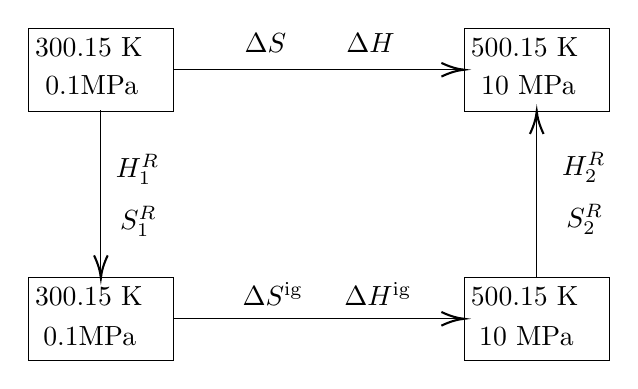
\begin{tikzpicture}[x=0.75pt,y=0.75pt,yscale=-1,xscale=1]
%uncomment if require: \path (0,310); %set diagram left start at 0, and has height of 310

%Shape: Rectangle [id:dp7157481404736188] 
\draw   (138,36) -- (208,36) -- (208,76) -- (138,76) -- cycle ;
%Shape: Rectangle [id:dp4206699841536288] 
\draw   (138,156) -- (208,156) -- (208,196) -- (138,196) -- cycle ;
%Shape: Rectangle [id:dp5931824609872525] 
\draw   (348,36) -- (418,36) -- (418,76) -- (348,76) -- cycle ;
%Shape: Rectangle [id:dp41529041931457367] 
\draw   (348,156) -- (418,156) -- (418,196) -- (348,196) -- cycle ;
%Straight Lines [id:da35176860331240367] 
\draw    (208,56) -- (346,56) ;
\draw [shift={(348,56)}, rotate = 180] [color={rgb, 255:red, 0; green, 0; blue, 0 }  ][line width=0.75]    (10.93,-3.29) .. controls (6.95,-1.4) and (3.31,-0.3) .. (0,0) .. controls (3.31,0.3) and (6.95,1.4) .. (10.93,3.29)   ;
%Straight Lines [id:da0016145845288071392] 
\draw    (208,176) -- (346,176) ;
\draw [shift={(348,176)}, rotate = 180] [color={rgb, 255:red, 0; green, 0; blue, 0 }  ][line width=0.75]    (10.93,-3.29) .. controls (6.95,-1.4) and (3.31,-0.3) .. (0,0) .. controls (3.31,0.3) and (6.95,1.4) .. (10.93,3.29)   ;
%Straight Lines [id:da7326401977633896] 
\draw    (173,75.63) -- (173,154.38) ;
\draw [shift={(173,156.38)}, rotate = 270] [color={rgb, 255:red, 0; green, 0; blue, 0 }  ][line width=0.75]    (10.93,-3.29) .. controls (6.95,-1.4) and (3.31,-0.3) .. (0,0) .. controls (3.31,0.3) and (6.95,1.4) .. (10.93,3.29)   ;
%Straight Lines [id:da20332604498771678] 
\draw    (383,156) -- (383,78) ;
\draw [shift={(383,76)}, rotate = 90] [color={rgb, 255:red, 0; green, 0; blue, 0 }  ][line width=0.75]    (10.93,-3.29) .. controls (6.95,-1.4) and (3.31,-0.3) .. (0,0) .. controls (3.31,0.3) and (6.95,1.4) .. (10.93,3.29)   ;

% Text Node
\draw (140,39.4) node [anchor=north west][inner sep=0.75pt]    {$300.15\ \mathrm{K}$};
% Text Node
\draw (145,57.4) node [anchor=north west][inner sep=0.75pt]    {$\mathrm{0.1MPa}$};
% Text Node
\draw (140,159.4) node [anchor=north west][inner sep=0.75pt]    {$300.15\ \mathrm{K}$};
% Text Node
\draw (144,178.4) node [anchor=north west][inner sep=0.75pt]    {$\mathrm{0.1MPa}$};
% Text Node
\draw (350,39.4) node [anchor=north west][inner sep=0.75pt]    {$500.15\ \mathrm{K}$};
% Text Node
\draw (355,57.4) node [anchor=north west][inner sep=0.75pt]    {$10\ \mathrm{MPa}$};
% Text Node
\draw (354,178.4) node [anchor=north west][inner sep=0.75pt]    {$10\ \mathrm{MPa}$};
% Text Node
\draw (350,159.4) node [anchor=north west][inner sep=0.75pt]    {$500.15\ \mathrm{K}$};
% Text Node
\draw (181,120.4) node [anchor=north west][inner sep=0.75pt]    {$S_{1}^{R}$};
% Text Node
\draw (179,95.4) node [anchor=north west][inner sep=0.75pt]    {$H_{1}^{R}$};
% Text Node
\draw (396,119.4) node [anchor=north west][inner sep=0.75pt]    {$S_{2}^{R}$};
% Text Node
\draw (394,94.4) node [anchor=north west][inner sep=0.75pt]    {$H_{2}^{R}$};
% Text Node
\draw (241,37.4) node [anchor=north west][inner sep=0.75pt]    {$\Delta S$};
% Text Node
\draw (290,37.4) node [anchor=north west][inner sep=0.75pt]    {$\Delta H$};
% Text Node
\draw (240,157.4) node [anchor=north west][inner sep=0.75pt]    {$\Delta S\mathrm{^{ig}}$};
% Text Node
\draw (289,157.4) node [anchor=north west][inner sep=0.75pt]    {$\Delta H^{\mathrm{ig}}$};
\end{tikzpicture}
\end{center}

	$T_{1} = 27+273.15\ \rm{K} = 300.15K$,$T_{2} = 227+273.15\ \rm{K} = 500.15K$,先根据数据计算对比状态:
\begin{equation*}
	T_{r1} = \dfrac{T_1}{T_{c}}=\dfrac{300.15}{417}=0.720
\end{equation*}
\begin{equation*}
	p_{r1} = \dfrac{p_1}{p_{c}}=\dfrac{0.1}{7.701}=0.0130
\end{equation*}

\begin{equation*}
	T_{r2} = \dfrac{T_2}{T_{c}}=\dfrac{500.15}{417}=1.199
\end{equation*}
\begin{equation*}
	p_{r2} = \dfrac{p_2}{p_{c}}=\dfrac{10}{7.701}=1.299
\end{equation*}
这里利用普遍化第二Virial系数法进行计算,首先计算Virial系数:
\begin{equation*}
	B^{0}(T_{r}=0.720)=0.083-\dfrac{0.422}{T_{r}^{1.6}} = 0.083-\dfrac{0.422}{0.720^{1.6}}=-0.631
\end{equation*}
\begin{equation*}
	B^{1}(T_{r}=0.720)=0.139-\dfrac{0.172}{T_{r}^{4.2}} = 0.139-\dfrac{0.172}{0.720^{4.2}}=0.0544
\end{equation*}

\begin{equation*}
	B^{0}(T_{r}=1.199)=0.083-\dfrac{0.422}{T_{r}^{1.6}} = 0.083-\dfrac{0.422}{1.199^{1.6}}=-0.233
\end{equation*}
\begin{equation*}
	B^{1}(T_{r}=1.199)=0.139-\dfrac{0.172}{T_{r}^{4.2}} = 0.139-\dfrac{0.172}{1.199^{4.2}}=0.0587
\end{equation*}
求导都可知:
\begin{equation*}
	\qd{B^{0}}{T_{r}}=\dfrac{0.675}{T_{r}^{2.6}},\quad \qd{B^{0}}{T_{r}}(T_{r}=0.720)=\dfrac{0.675}{0.720^{2.6}} =1.59,\quad \qd{B^{0}}{T_{r}}(T_{r}=1.199)=\dfrac{0.675}{1.199^{2.6}} = 0.421
\end{equation*}
\begin{equation*}
	\qd{B^{1}}{T_{r}}=\dfrac{0.722}{T_{r}^{5.2}},\quad \qd{B^{0}}{T_{r}}(T_{r}=0.720)=\dfrac{0.722}{0.720^{5.2}} = 3.98,\quad \qd{B^{0}}{T_{r}}(T_{r}=1.199)=\dfrac{0.722}{1.199^{5.2}} = 0.281
\end{equation*}
这样直接带入公式即可:
\begin{equation*}
\begin{aligned}
		\dfrac{H^{R}_{1}}{RT}&=p_{r}\pqty{\dfrac{B^{0}}{T_{r}}-\qd{B^{0}}{T_{r}}+\omega\pqty{\dfrac{B^{1}}{T_{r}}-\qd{B^{1}}{T_{r}}}}\\
		&=0.0130\pqty{\dfrac{-0.631}{0.720}-1.59 +0.073\pqty{\dfrac{0.0544}{0.720}-3.98}}\\
		&=-0.358\\
		\dfrac{S^{R}_{1}}{R} &=-p_{r}\pqty{\qd{B^{0}}{R}+\omega\qd{B^{1}}{T_{r}}}\\
		&=-0.0130\pqty{1.59 +0.073\times 3.98}\\
		&=-0.0244
\end{aligned}
\end{equation*}

\begin{equation*}
\begin{aligned}
		\dfrac{H^{R}_{2}}{RT}&=p_{r}\pqty{\dfrac{B^{0}}{T_{r}}-\qd{B^{0}}{T_{r}}+\omega\pqty{\dfrac{B^{1}}{T_{r}}-\qd{B^{1}}{T_{r}}}}\\
		&=1.299\pqty{\dfrac{-0.233}{1.199}-0.421+0.073\pqty{\dfrac{0.0587}{1.199}-0.281}}\\
		&=-0.821\\
		\dfrac{S^{R}_{2}}{R} &=-p_{r}\pqty{\qd{B^{0}}{R}+\omega\qd{B^{1}}{T_{r}}}\\
		&=-1.299\pqty{0.421 +0.073\times 0.281}\\
		&=-0.574
\end{aligned}
\end{equation*}

这样一来,移项即可求得:
\begin{equation*}
	H^{R}_{1} = -89.3{\rm{J}\cdot\rm{mol}^{-1}}\quad S^{R}_{1}=0.203\rm{J}\cdot\rm{mol}^{-1}\cdot\rm{K}^{-1}
\end{equation*}
\begin{equation*}
	H^{R}_{2} = -3415{\rm{J}\cdot\rm{mol}^{-1}}\quad S^{R}_{2}=-4.768\rm{J}\cdot\rm{mol}^{-1}\cdot\rm{K}^{-1}
\end{equation*}
对于理想气体的变温变压过程,根据化学热力学中的公式可知:
\begin{equation*}
\begin{aligned}
	\Delta H^{{\rm{ig}}}&=\int_{T_{1}}^{T_{2}}C_{p}^{{\rm{ig}}}{\rm{d}}T =\int_{300.15}^{500.15}(31.696+10.144\times 10^{-3}T-4.038\times 10^{-6}T^{2}){\rm{d}}T =7019{\rm{J}\cdot\rm{mol}^{-1}}\\
		\Delta S^{{\rm{ig}}}&=\int_{T_{1}}^{T_{2}}\dfrac{C_{p}^{{\rm{ig}}}}{T}{\rm{d}}T+R\ln{\dfrac{p_{1}}{p_{2}}}=\int_{300.15}^{500.15}\dfrac{31.696+10.144\times 10^{-3}T-4.038\times 10^{-6}T^{2}}{T}{\rm{d}}T+8.314\ln{\dfrac{0.1}{10}}\\
		&=-20.4\rm{mol}^{-1}\cdot\rm{K}^{-1}
\end{aligned}
\end{equation*}
综上,整个过程的焓、熵变化为:
\begin{equation*}
	\begin{aligned}
		\Delta H &= -H^{R}_{1}+\Delta H^{{\rm{ig}}}+H^{R}_{2}=89.3+7019-3415\ {\rm{J}\cdot\rm{mol}^{-1}}= 3693.3 {\rm{J}\cdot\rm{mol}^{-1}}\\
		\Delta S &= -S^{R}_{1}+\Delta S^{{\rm{ig}}}+S^{R}_{2}=  -0.203-20.4-4.768\ \rm{mol}^{-1}\cdot\rm{K}^{-1} = -25.071\rm{mol}^{-1}\cdot\rm{K}^{-1}\\
	\end{aligned}
\end{equation*}

\end{solution}



\begin{problem}
	试采用RK方程计算在227\ssd、5MPa下的气相正丁烷的剩余焓和剩余熵。正丁烷的临界参数和偏心因子分别为:
$T_{c}$=425.2K ,$p_{c}$=3.800MPa ,$\omega$=0.193
\end{problem}

\begin{solution}
	$T = 227+273.15 \ \rm{K} = 500.15\rm{K}$,利用R-K方程,先计算物性常数:
	\begin{equation*}
		a = 0.42748\dfrac{R^{2}T_{c}^{2.5}}{p_{c}} = 0.42748\dfrac{8.314^{2}\times 425.2^{2.5}}{3.800}\rm{Pa}\cdot \rm{K}^{0.5}\cdot\rm{m}^{6}\cdot\rm{Mmol}^{-2}=29.0\rm{Pa}\cdot \rm{K}^{0.5}\cdot\rm{m}^{6}\cdot\rm{mol}^{-2}
	\end{equation*}
	\begin{equation*}
			b = 0.08664\times\dfrac{RT_{c}}{p_{c}} = 0.08664\times\dfrac{8.314\times 425.2}{3.800}\rm{m}^{3}\cdot\rm{Mmol}^{-1}=8.06\times 10^{-5}\rm{m}^{3}\cdot\rm{mol}^{-1}
	\end{equation*}
	然后列出R-K方程:
	\begin{equation}
		p  = \dfrac{RT}{V-b}-\dfrac{a}{T^{0.5}V(V+b)} 
	\end{equation}
	然后利用计算机解之\footnote{利用Patrick Barrie's program for solving cubic equations of state,具体网址在\href{http://www.mathaddict.net/realgas4.htm}{http://www.mathaddict.net/realgas4.htm}} ,得到:
	\begin{equation*}
		V_{m} = 0.000570{\rm{m}}^{3}\cdot{\rm{mol}}^{-1}
	\end{equation*}
	然后带入公式即可求出:
	\begin{equation*}
		\begin{aligned}
			H^{R} &=pV_{m}-RT-\dfrac{3a}{2T^{0.5}b}\ln{\pqty{1+\dfrac{b}{V_{m}}}} \\
			&=5\times 10^{6}\times 0.000570 -8.314\times 500.15-\dfrac{3\times 29.0}{2\times 500.15^{0.5}\times 8.06\times 10^{-5}}\ln{\pqty{1+\dfrac{8.06\times 10^{-5}}{0.000570}}} \\
			&=-4500 {\rm{J}\cdot\rm{mol}^{-1}}\\
			S^{R} &= R\ln{(V_{m}-b)}-R\ln{\dfrac{RT}{p}}-\dfrac{a}{2T^{1.5}b}\ln{\pqty{1+\dfrac{b}{V_{m}}}}\\
	&= 8.314\ln{(0.000570-8.06\times 10^{-5})}-8.314\ln{\dfrac{8.314\times 500.15}{5\times 10^{6}}}\\
	&\quad \quad \quad -\dfrac{29.0}{2\times 500.15^{1.5}\times 8.06\times 10^{-5}}\ln{\pqty{1+\dfrac{8.06\times 10^{-5}}{0.000570}}}=-6.54\rm{mol}^{-1}\cdot\rm{K}^{-1}
		\end{aligned}
	\end{equation*}
\end{solution}

\begin{problem}
	假设125\ssd、10MPa下的丙烯服从R-K状态方程,试运用 R-K 方程求算该状态下的丙烯的剩余焓与剩余熵。该状态下的丙烯的$V_{m} = 1.42\times 10^{-4}\rm{m}^{3}\cdot \rm{mol}$,丙烯的临界参数和偏心因子分别为:
$T_{c}$=3650K , $p_{c}$=4.620MPa , $\omega$=0.193

\end{problem}
\begin{solution}
	$T = 125+273.15\ \rm{K} = 398.15\rm{K}$利用R-K方程,还是先计算物性常数:
	\begin{equation*}
		a = 0.42748\dfrac{R^{2}T_{c}^{2.5}}{p_{c}} = 0.42748\dfrac{8.314^{2}\times 365.0^{2.5}}{4.620}\rm{Pa}\cdot \rm{K}^{0.5}\cdot\rm{m}^{6}\cdot\rm{Mmol}^{-2}=16.28\rm{Pa}\cdot \rm{K}^{0.5}\cdot\rm{m}^{6}\cdot\rm{mol}^{-2}
	\end{equation*}
	\begin{equation*}
			b = 0.08664\times\dfrac{RT_{c}}{p_{c}} = 0.08664\times\dfrac{8.314\times 365.0}{4.620}\rm{m}^{3}\cdot\rm{Mmol}^{-1}=5.691\times 10^{-5}\rm{m}^{3}\cdot\rm{mol}^{-1}
	\end{equation*}
	如上题,同样得到:
	\begin{equation*}
		V_{m} = 0.0001360{\rm{m}}^{3}\cdot{\rm{mol}}^{-1}
	\end{equation*}
	然后带入公式即可求出:
	\begin{equation*}
		\begin{aligned}
			H^{R} &=pV_{m}-RT-\dfrac{3a}{2T^{0.5}b}\ln{\pqty{1+\dfrac{b}{V_{m}}}} \\
			&=10\times 10^{6}\times 0.0001360 -8.314\times 398.15-\dfrac{3\times 16.28}{2\times 398.15^{0.5}\times 5.691\times 10^{-5}}\ln{\pqty{1+\dfrac{5.691\times 10^{-5}}{0.0001360}}} \\
			&= -9468 {\rm{J}\cdot\rm{mol}^{-1}}\\
		\end{aligned}
	\end{equation*}
	\begin{equation*}
		\begin{aligned}
			S^{R} &= R\ln{(V_{m}-b)}-R\ln{\dfrac{RT}{p}}-\dfrac{a}{2T^{1.5}b}\ln{\pqty{1+\dfrac{b}{V_{m}}}}\\
	&= 8.314\ln{(0.0001360-5.691\times 10^{-5})}-8.314\times\ln{\dfrac{8.06\times 10^{-5}\times 398.15}{10\times 10^{6}}}\\
	&\quad \quad \quad -\dfrac{16.28}{2\times 398.15^{1.5}\times5.691\times 10^{-5}}\ln{\pqty{1+\dfrac{5.691\times 10^{-5}}{0.0001360}}}=-18.20\rm{mol}^{-1}\cdot\rm{K}^{-1}
		\end{aligned}
	\end{equation*}
\end{solution}
\chapter{2022年4月14日\quad 晴$^{\star}$}
本次作业的第一题是上一次作业的倒数第二题,剩下两题解答如下:
\begin{problem}
	试用普遍化方法计算二氧化碳在473.2K、30MPa下的焓与熵。二氧化碳的临界参数和偏心因子分别为:
$T_{c}=304.2\ce{K},p_{c}=7.376{\rm{MPa}},\omega =0.225$。已知在相同条件下,二氧化碳处于理想状态的焓为$8377\rm{J}\cdot\rm{mol}^{-1}$,熵为$-25.86\rm{J}\cdot\rm{mol}^{-1}\cdot\rm{K}^{-1}$。
\end{problem}
\begin{solution}
先根据数据计算对比状态:
\begin{equation*}
	T_{r} = \dfrac{T}{T_{c}}=\dfrac{473.2}{304.2}=1.556
\end{equation*}
\begin{equation*}
	p_{r} = \dfrac{p}{p_{c}}=\dfrac{30}{7.376}=4.067
\end{equation*}
然后计算Virial系数:
\begin{equation*}
	B^{0}(T_{r}=1.556)=0.083-\dfrac{0.422}{T_{r}^{1.6}} = 0.083-\dfrac{0.422}{1.556^{1.6}}=-0.125
\end{equation*}
\begin{equation*}
	B^{1}(T_{r}=1.556)=0.139-\dfrac{0.172}{T_{r}^{4.2}} = 0.139-\dfrac{0.172}{1.556^{4.2}}=0.112
\end{equation*}
求导可知:
\begin{equation*}
	\qd{B^{0}}{T_{r}}=\dfrac{0.675}{T_{r}^{2.6}},\quad \qd{B^{0}}{T_{r}}(T_{r}=1.556)=\dfrac{0.675}{1.556^{2.6}} =0.214
\end{equation*}
\begin{equation*}
	\qd{B^{1}}{T_{r}}=\dfrac{0.722}{T_{r}^{5.2}},\quad \qd{B^{0}}{T_{r}}(T_{r}=1.556)=\dfrac{0.722}{1.556^{5.2}} = 0.0725
\end{equation*}
这样直接带入公式即可:
\begin{equation*}
\begin{aligned}
		\dfrac{H^{R}}{RT}&=p_{r}\pqty{\dfrac{B^{0}}{T_{r}}-\qd{B^{0}}{T_{r}}+\omega\pqty{\dfrac{B^{1}}{T_{r}}-\qd{B^{1}}{T_{r}}}}\\
		&=4.067\pqty{\dfrac{-0.125}{1.556}-0.214 +0.225\pqty{\dfrac{0.112}{1.556}-0.0725}}\\
		&=-1.197\\
\end{aligned}
\end{equation*}
\begin{equation*}
\begin{aligned}
		\dfrac{S^{R}}{R} &=-p_{r}\pqty{\qd{B^{0}}{R}+\omega\qd{B^{1}}{T_{r}}}\\
		&=-4.067\pqty{0.214+0.225\times 0.0725}\\
		&=-0.9367
\end{aligned}
\end{equation*}
这样就可以得到:
\begin{equation*}
\begin{aligned}
	H(473.2\ce{K},30\ce{MPa}) &= H^{R}+H^{\ce{ig}}(473.2\ce{K},30\ce{MPa})\\
	&=-1.197\times 8.314\times 473.2+8377\ \rm{J}\cdot\rm{mol}^{-1}\\
	&=3668\rm{J}\cdot\rm{mol}^{-1}\\
	S(473.2\ce{K},30\ce{MPa})&= S^{R}+S^{\ce{ig}}(473.2\ce{K},30\ce{MPa})\\
	&=-0.9367\times 8.314-25.86 \ \rm{J}\cdot\rm{mol}^{-1}\cdot\rm{K}^{-1}\\
	&=-33.65\rm{J}\cdot\rm{mol}^{-1}\cdot\rm{K}^{-1}
\end{aligned}
\end{equation*}

\end{solution}


\begin{problem}
	试用普遍化第二维里系数法计算丙烷气体在378K、0.507MPa下的剩余焓。已知丙烷的临界常数:$T_{c}=369.8\ce{K},p_{c}=4.246{\rm{MPa}},\omega =0.152$。
\end{problem}
\begin{solution}
先根据数据计算对比状态:
\begin{equation*}
	T_{r} = \dfrac{T}{T_{c}}=\dfrac{378}{369.8}=1.02
\end{equation*}
\begin{equation*}
	p_{r} = \dfrac{p}{p_{c}}=\dfrac{0.507}{4.246}=0.119
\end{equation*}
然后计算Virial系数:
\begin{equation*}
	B^{0}(T_{r}=1.02)=0.083-\dfrac{0.422}{T_{r}^{1.6}} = 0.083-\dfrac{0.422}{1.02^{1.6}}=-0.326
\end{equation*}
\begin{equation*}
	B^{1}(T_{r}=1.02)=0.139-\dfrac{0.172}{T_{r}^{4.2}} = 0.139-\dfrac{0.172}{1.02^{4.2}}=-0.0162
\end{equation*}
求导可得:
\begin{equation*}
	\qd{B^{0}}{T_{r}}=\dfrac{0.675}{T_{r}^{2.6}},\quad \qd{B^{0}}{T_{r}}(T_{r}=1.02)=\dfrac{0.675}{1.02^{2.6}} =0.641
\end{equation*}
\begin{equation*}
	\qd{B^{1}}{T_{r}}=\dfrac{0.722}{T_{r}^{5.2}},\quad \qd{B^{0}}{T_{r}}(T_{r}=1.02)=\dfrac{0.722}{1.02^{5.2}} = 0.651
\end{equation*}
这样直接带入公式即可:
\begin{equation*}
\begin{aligned}
		\dfrac{H^{R}}{RT}&=p_{r}\pqty{\dfrac{B^{0}}{T_{r}}-\qd{B^{0}}{T_{r}}+\omega\pqty{\dfrac{B^{1}}{T_{r}}-\qd{B^{1}}{T_{r}}}}\\
		&=0.119\pqty{\dfrac{-0.326}{1.02}-0.641 +0.152\pqty{\dfrac{-0.0162}{1.02}-0.651}}\\
		&=-0.126\\
		\dfrac{S^{R}}{R} &=-p_{r}\pqty{\qd{B^{0}}{R}+\omega\qd{B^{1}}{T_{r}}}\\
		&=-0.119\pqty{0.641+0.152\times 0.651}\\
		&=-0.0881\\
\end{aligned}
\end{equation*}
这样就得到:\begin{equation*}
	H^{R} = -397{\rm{J}\cdot\rm{mol}^{-1}}, \quad S^{R} = 0.732\rm{J}\cdot\rm{mol}^{-1}\cdot\rm{K}^{-1}
\end{equation*}
\end{solution}



\chapter{2022年4月21日\quad 晴$^\dag$}
\begin{problem}
	某容器内的液态水和蒸汽在1MPa下处于平衡状态,质量为1kg。假如容器内液体和蒸汽各占一半体积,试求容器内的液态水和蒸汽的总焓。
	
已知:饱和水蒸汽表,1MPa时,$H_{l} = 762.81{\rm{kJ}}\cdot{\rm{kg}}^{-1}$、$H_{g} = 2778.1{\rm{kJ}}\cdot{\rm{kg}}^{-1}$、$V_{l} = 1.1273{\rm{cm}}^{3}\cdot{\rm{g}}^{-1}$、$V_{g} = 194.4{\rm{cm}}^{3}\cdot{\rm{g}}^{-1}$
\end{problem}
\begin{solution}
	设水饱和蒸汽占全体的质量比重\footnote{也叫\textcolor{myblu}{干度},这里不这么称呼是为了减少边缘名词个数}为$x$,这样就可以根据体积相等给出以下关系式:
	\begin{equation*}
		xV_{g} = (1-x)V_{l}
	\end{equation*}
	代入数据,可得:
	\begin{equation*}
		194.4x=1.1273(1-x)
	\end{equation*}
	解得$x = 0.005765$
那么体系的总焓$H$可以表示为以下式子:
	\begin{equation*}
		\begin{aligned}
			H &=(1-x)H_{l}+ xH_{g}\\
			&=(1-0.005765)\times 762.81+0.005765\times 2778.1\  {\rm{kJ}}\cdot{\rm{kg}}^{-1} = 774.43{\rm{kJ}}\cdot{\rm{kg}}^{-1}
		\end{aligned}
	\end{equation*}
\end{solution}




\begin{problem}
	假设二氧化碳服从RK状态方程,计算50\ssd、10.13MPa时二氧化碳的逸度。二氧化碳的临界参数和偏心因子分别为:$T_{c}$=304.2K,$p_{c}$=7.376MPa,$\omega$=0.225
\end{problem}

\begin{solution}
	先计算物性常数:
	\begin{equation*}
		a = 0.42748\dfrac{R^{2}T_{c}^{2.5}}{p_{c}} = 0.42748\times\dfrac{8.314^{2}304.2^{2.5}}{7.376}\rm{Pa}\cdot \rm{K}^{0.5}\cdot\rm{m}^{6}\cdot\rm{Mmol}^{-1}= 6.466\rm{Pa}\cdot \rm{K}^{0.5}\cdot\rm{m}^{6}\cdot\rm{mol}^{-1}
	\end{equation*}
	\begin{equation*}
		b = 0.08664\times\dfrac{RT_{c}}{p_{c}} = 0.08664\times\dfrac{8.314\times 304.2}{7.376}\rm{m}^{3}\cdot\rm{Mmol}^{-1}= 29.71\times 10^{-6}\rm{m}^{3}\cdot\rm{mol}^{-1}
	\end{equation*}


待求温度为$T = 50+273.15\ \rm{K} = 323.15\rm{K}$,然后列出R-K方程,并反解\footnote{仍然利用Patrick Barrie's program for solving cubic equations of state,具体网址在\href{http://www.mathaddict.net/realgas4.htm}{http://www.mathaddict.net/realgas4.htm}}得:$V_{m} = 0.0001082\rm{m}^{3}\cdot\rm{mol}^{-1}$此时压缩因子为$Z = 0.4079$

%10.13\times 10^{6} = \dfrac{8.314\times 323.15}{V-29.71\times 10^{-6}}-\dfrac{6.4661}{323.15^{0.5}V(V+29.71\times 10^{-6})}
然后带入逸度因子的求算公式得到:
\begin{equation*}
	\begin{aligned}
		\ln{\varphi} = \ln{\dfrac{f}{p}} &= Z-1-\ln(Z - \dfrac{bp}{RT})-\dfrac{a}{bRT^{1.5}}\ln(1+\dfrac{b}{V_{m}})\\
		&=0.4079-1-\ln(0.4079 - \dfrac{29.71\times 7.376}{8.314\times 304.2})\\
		&-\dfrac{6.466}{29.71\times 10^{-6}\times 8.314\times 323.15^{1.5}}\ln(1+\dfrac{29.71\times 10^{-6}}{0.0001082})\\
		&=-0.6536
	\end{aligned}
\end{equation*}
这样就可知:
\begin{equation*}
	f = p\times e^{-0.6536} = 7.376\times e^{-0.6536} \rm{MPa}=3.837MPa
\end{equation*}
\end{solution}
\begin{problem}
试计算液态水在30\ssd 下,压力分别为(a)饱和蒸气压(b)$100\times 10^{5}$Pa下的逸度和逸度系数。
已知:
\begin{enumerate}
	\item 水在30\ssd 时的饱和蒸气压$p^{s} = 0.0424\times 10^{5}$Pa。
	\item 30\ssd ,$0\sim 100\times 10^{5}$Pa范围内将液态水的摩尔体积视为常数,其值为$0.01809 {\rm{m}}^{3}\cdot {\rm{kmol}}^{-1}$。
	\item $100\times 10^{5}$Pa以下的水蒸气可以视为理想气体。
\end{enumerate}
\end{problem}


\begin{solution}
	\begin{enumerate}
		\item[(a)] 当此之时,30\ssd 液态水之气压为饱和蒸气压,故其处于相平衡状态;又由于其压力较小,饱和水蒸气视作理想气体,故$f = p^{s} =0.0424\times 10^{5}\ce{Pa},\ \varphi = 1$
		\item[(b)] 此时压力$p = 100\times 10^{5}\rm{Pa}$,所以不再处于相平衡状态。那么:
		\begin{equation*}
			\begin{aligned}
				\ln{\varphi} = \ln{\dfrac{f}{p}} &= \int_{p^{s}}^{p} \pqty{\dfrac{V_{m}}{RT} - \dfrac{1}{p}}\ce{d}p\\
				&=\int_{0.0424\times 10^{5}{\rm{Pa}}}^{100\times 10^{5}\ce{Pa}}\pqty{\dfrac{0.01809\times 10^{-3}{\rm{m}}^{3}\cdot {\rm{mol}}^{-1}}{8.314\times (273.15+30)\ce{Pa}\cdot\ce{m}^{3}\cdot\ce{mol}^{-1}}-\dfrac{1}{p}}\ce{d}p\\
				&=-7.694
			\end{aligned}
		\end{equation*}
		明显有$\varphi = e^{-7.694} = 0.0004555$,且有:
		\begin{equation*}
			f = p\times e^{-7.694} = 100\times 10^{5}\times e^{-7.694}\ce{Pa} = 4555\ce{Pa}
		\end{equation*}
	\end{enumerate}
\end{solution}

\chapter{2022年5月05日\quad 晴}

\begin{problem}
	某厂用功率为2.4kW的泵将95\ssd 水从贮水罐压到换热器,水流量为3.2$\ce{kg}\cdot\ce{s}^{-1}$。在换热器中以720$\ce{kJ}\cdot\ce{s}^{-1}$的速率将水冷却,冷却后水送入比第一贮水罐高20m的第二贮水罐,求送入第二贮水罐的水温。(已知水的恒压热容为$C_{p}=4.187\ce{kJ}\cdot\ce{kg}^{-1}\cdot\ce{K}^{-1}$)
\end{problem}

\begin{solution}
	列出能量守恒关系,视流速不改变,动能改变项为0,则:
	\begin{equation*}
		\begin{aligned}
			\dfrac{\Delta H}{m} &= \dfrac{Q}{m} + \dfrac{W_{s}}{m} - g\Delta z -\dfrac{1}{2}\Delta u^{2}  \\
			&=-\dfrac{720}{3.2}+\dfrac{2.4}{3.2}-9.81\times 10^{-3}\times 20 -0 \ \ce{J}\cdot\ce{kg}^{-1}\\
			&=-224\ce{J}\cdot\ce{g}^{-1} = C_{p}(T_{2}-T_{1}) = C_{p}(\theta_{2}-\theta_{1}) =4.187\times(\theta_{2}-95\sssd)
		\end{aligned}
	\end{equation*}
	解得:$\theta_{2} = 41.5\sssd $
\end{solution}

\begin{problem}
	有一水平敷设的热交换器,其进、出口的截面积相等,空气进入时的温度、压强和流速分别为303K、0.103MPa和10$\ce{m}\cdot\ce{s}^{-1}$,离开时的温度和压强为403K和0.102MPa。已知空气的恒压平均热容为$C_{p}=1.005\ce{kJ}\cdot\ce{kg}^{-1}\cdot\ce{K}^{-1}$,试计算:
	\begin{enumerate}
		\item 当空气的质量流量为80$\ce{kg}\cdot\ce{h}^{-1}$时从热交换器吸收多少热量?
		\item 若热交换器垂直安装,高6m,空气自下而上流动,则空气离开热交换器时吸收的热量为多少?
	\end{enumerate}
\end{problem}
\begin{solution}
	\begin{enumerate}
		\item 首先计算空气流出时的流速:
	\begin{equation*}
		u_{2} = u_{1}\dfrac{p_{1}T_{2}}{p_{2}T_{1}} =10 \times\dfrac{403\cdot 0.103}{303\cdot 0.102}\ \ce{m}\cdot\ce{s}^{-1}=13\ce{m}\cdot\ce{s}^{-1}
	\end{equation*}
	热交换器不做功,此时根据能量衡算式:
	\begin{equation*}
		\begin{aligned}
			\dfrac{\Delta H}{m} &= \dfrac{Q}{m} + \dfrac{W_{s}}{m} + g\Delta z +\dfrac{1}{2}\Delta u^{2}  \\
			C_{p}(T_{2}-T_{1})=  1.005\times(403\ce{K}-303\ce{K})\ce{J}\cdot\ce{g}^{-1}&= \dfrac{Q}{m}+0+0+\dfrac{1}{2}\times (13^{2}-10^{2})\times 10^{-3}\ce{kJ}\cdot\ce{kg}^{-1}
		\end{aligned}
	\end{equation*}
	解得:$\dfrac{Q}{m} = 100.5\ce{kJ}\cdot\ce{kg}^{-1}$。则每小时,空气从热交换机吸收热量为:
	\begin{equation*}
		Q_{h} = 100.5\ce{kJ}\cdot\ce{kg}^{-1}\times 80\ce{kg}\cdot\ce{h}^{-1}=8040\ce{kJ}\cdot\ce{h}^{-1}
	\end{equation*}
		\item 根据能量衡算式:
	\begin{equation*}
		\begin{aligned}
			\dfrac{\Delta H}{m} &= \dfrac{Q}{m} + \dfrac{W_{s}}{m} + g\Delta z +\dfrac{1}{2}\Delta u^{2}  \\
			1.005\times(403\ce{K}-303\ce{K})\ce{J}\cdot\ce{g}^{-1}&= \dfrac{Q}{m}+0+9.81\times 6\times 10^{-3}+\dfrac{1}{2}\times (13^{2}-10^{2})\times 10^{-3}\ce{kJ}\cdot\ce{kg}^{-1}
		\end{aligned}
	\end{equation*}
	则每小时,空气从热交换机吸收热量为:
	\begin{equation*}
		Q_{h} = 100.4\ce{kJ}\cdot\ce{kg}^{-1}\times 80\ce{kg}\cdot\ce{h}^{-1}=8035\ce{kJ}\cdot\ce{h}^{-1}
	\end{equation*}

	\end{enumerate}
\end{solution}

\begin{problem}
	有一个使用蒸气压缩机将海水脱盐来制备淡水的装置。若水蒸气稳定流入压缩机,其压力为0.1MPa, 温度为103.2\ssd 。水蒸气被绝热压缩到0.14MPa,如果压缩机的效率为70\%,试求:
	\begin{enumerate}
		\item 压缩机出口处水蒸气的温度;
		\item 压缩1kg水蒸气所需要的功。
	\end{enumerate}
\end{problem}
\begin{solution}

\begin{center}
	

\tikzset{every picture/.style={line width=0.75pt}} %set default line width to 0.75pt        

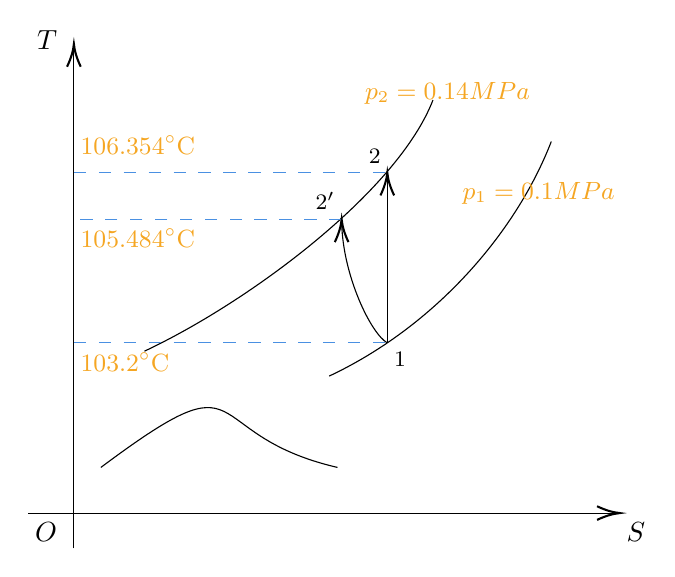
\begin{tikzpicture}[x=0.75pt,y=0.75pt,yscale=-1,xscale=1]
%uncomment if require: \path (0,268); %set diagram left start at 0, and has height of 268

%Straight Lines [id:da9679663496758055] 
\draw    (33,258) -- (33,17) ;
\draw [shift={(33,15)}, rotate = 90] [color={rgb, 255:red, 0; green, 0; blue, 0 }  ][line width=0.75]    (10.93,-3.29) .. controls (6.95,-1.4) and (3.31,-0.3) .. (0,0) .. controls (3.31,0.3) and (6.95,1.4) .. (10.93,3.29)   ;
%Straight Lines [id:da4968304994846491] 
\draw    (11,241) -- (294,241) ;
\draw [shift={(296,241)}, rotate = 180] [color={rgb, 255:red, 0; green, 0; blue, 0 }  ][line width=0.75]    (10.93,-3.29) .. controls (6.95,-1.4) and (3.31,-0.3) .. (0,0) .. controls (3.31,0.3) and (6.95,1.4) .. (10.93,3.29)   ;
%Curve Lines [id:da5754375228814621] 
\draw    (46,219) .. controls (121,163) and (91,203) .. (160,219) ;
%Curve Lines [id:da5411674890145801] 
\draw    (67,163) .. controls (118,139) and (189,86) .. (206,42) ;
%Curve Lines [id:da44807281212893413] 
\draw    (156,175) .. controls (207,151) and (246,106) .. (263,62) ;
%Straight Lines [id:da7552092789097284] 
\draw [color={rgb, 255:red, 74; green, 144; blue, 226 }  ,draw opacity=1 ] [dash pattern={on 4.5pt off 4.5pt}]  (33,77) -- (184,77) ;
%Straight Lines [id:da7269015316192289] 
\draw [color={rgb, 255:red, 74; green, 144; blue, 226 }  ,draw opacity=1 ] [dash pattern={on 4.5pt off 4.5pt}]  (33,159) -- (184,159) ;
%Straight Lines [id:da5531026230699259] 
\draw [color={rgb, 255:red, 74; green, 144; blue, 226 }  ,draw opacity=1 ] [dash pattern={on 4.5pt off 4.5pt}]  (162,99.5) -- (33,99.5) ;
%Straight Lines [id:da01789249164191098] 
\draw    (184,159) -- (184,79) ;
\draw [shift={(184,77)}, rotate = 90] [color={rgb, 255:red, 0; green, 0; blue, 0 }  ][line width=0.75]    (10.93,-3.29) .. controls (6.95,-1.4) and (3.31,-0.3) .. (0,0) .. controls (3.31,0.3) and (6.95,1.4) .. (10.93,3.29)   ;
%Curve Lines [id:da13762490556360163] 
\draw    (184,159) .. controls (176.2,154.61) and (162.7,126.93) .. (162.03,101.46) ;
\draw [shift={(162,99.5)}, rotate = 90] [color={rgb, 255:red, 0; green, 0; blue, 0 }  ][line width=0.75]    (10.93,-3.29) .. controls (6.95,-1.4) and (3.31,-0.3) .. (0,0) .. controls (3.31,0.3) and (6.95,1.4) .. (10.93,3.29)   ;

% Text Node
\draw (14,7.4) node [anchor=north west][inner sep=0.75pt]    {$T$};
% Text Node
\draw (298,244.4) node [anchor=north west][inner sep=0.75pt]    {$S$};
% Text Node
\draw (13,244.4) node [anchor=north west][inner sep=0.75pt]    {$O$};
% Text Node
\draw (219,80.4) node [anchor=north west][inner sep=0.75pt]  [font=\small,color={rgb, 255:red, 245; green, 166; blue, 35 }  ,opacity=1 ]  {$p_{1} =0.1MPa$};
% Text Node
\draw (172,32.4) node [anchor=north west][inner sep=0.75pt]  [font=\small,color={rgb, 255:red, 245; green, 166; blue, 35 }  ,opacity=1 ]  {$p_{2} =0.14MPa$};
% Text Node
\draw (35,162.4) node [anchor=north west][inner sep=0.75pt]  [font=\small,color={rgb, 255:red, 245; green, 166; blue, 35 }  ,opacity=1 ]  {$103.2\sssd$};
% Text Node
\draw (35,102.9) node [anchor=north west][inner sep=0.75pt]  [font=\small,color={rgb, 255:red, 245; green, 166; blue, 35 }  ,opacity=1 ]  {$105.484\sssd$};
% Text Node
\draw (35,57.9) node [anchor=north west][inner sep=0.75pt]  [font=\small,color={rgb, 255:red, 245; green, 166; blue, 35 }  ,opacity=1 ]  {$106.354\sssd $};
% Text Node
\draw (186,162.4) node [anchor=north west][inner sep=0.75pt]  [font=\footnotesize]  {$1$};
% Text Node
\draw (160,96.1) node [anchor=south east] [inner sep=0.75pt]  [font=\footnotesize]  {$2'$};
% Text Node
\draw (182,73.6) node [anchor=south east] [inner sep=0.75pt]  [font=\footnotesize]  {$2$};
\end{tikzpicture}
\end{center}

	根据题目信息,流入压缩机时水蒸气温度$\theta_{1}=103.2 \sssd $,压力$p_{1} = 0.1\ce{MPa}$此时查表\footnote{利用网站\href{https://www.spiraxsarco.com/resources-and-design-tools/steam-tables/superheated-steam-region}{https://www.spiraxsarco.com/resources-and-design-tools/steam-tables/superheated-steam-region}进行计算} 可知,焓$H_{1} = 2680.38\hdw$、熵$S_{1} = 7.32611\sdw$。整个过程为绝热压缩。如果此番压缩,又可逆,则此过程为等熵过程。在焓-熵图上体现为$a$过程。此时$2$点处的焓与熵查表可知为:$H_{2} = 2686.43\hdw$。温度也可知为$\theta_{2} = 106.354\sssd$
	
	但过程并非等熵过程,若设在题目所给条件下达到的状态为$2'$,那么根据压缩机效率之定义:
	\begin{equation*}
		\eta = \dfrac{-W_{s}}{-W_{s,r}} = \dfrac{H_{1}-H_{2'}}{H_{1}-H_{2}}
		= \dfrac{2680.38-\dfrac{H_{2'}}{\hdw}}{2680.38-2686.43} =70\%
	\end{equation*}
	
	这样就解得:
	$H_{2'} = 2684.62\hdw$ ,根据此时的压力为$p_{2} = 0.14\ce{MPa}$,再查表可知:
	$S_{2'} = 7.32133\sdw$,温度$\theta_{2'} = 105.484\sssd$。
	于是:
	\begin{enumerate}
		\item 出口处水蒸气的温度为$\theta_{2'} = 105.484\sssd$
		\item 压缩机对外做功为:
		\begin{equation*}
			(w_{s})_{Q} = \eta w_{s,r} = 0.7\times (2680.38-2686.43) \hdw = -4.235\hdw
		\end{equation*}
	\end{enumerate}
	绝热损失功为:
	\begin{equation*}
		(w_{L})_{Q} = T_{0}\Delta S_{t} =  T_{0}\Delta S_{sys} = 298.15\times (7.32133-7.32611)\hdw = -1.425\hdw
	\end{equation*}
	所以所做的功应为$w = -(w_{L})_{Q} =  1.425\hdw $
\end{solution}

	
\begin{problem}
	将35kg、温度为700K的铸钢件放入135kg而温度为294K的油中冷却,已知铸钢和油的比热容分别为$C_{p_{\text{钢}}}=0.5\ce{kJ}\cdot\ce{kg}^{-1}\cdot\ce{K}^{-1}$和$C_{p_{\text{油}}}=2.5\ce{kJ}\cdot\ce{kg}^{-1}\cdot\ce{K}^{-1}$,若不计热损失,试求:
	\begin{enumerate}
		\item 铸钢件的熵变;
		\item 铸钢件和油的总熵变。
	\end{enumerate}
\end{problem}

\begin{solution}
	首先根据平衡条件,计算出终态温度$T$,视此变化等压,则:
	\begin{equation*}
		\begin{aligned}
			Q_{\text{油}} =m_{\text{油}}C_{p_{\text{油}}}(T-T_{\text{油}}) &= -m_{\text{钢}}C_{p_{\text{钢}}}(T-T_{\text{钢}})= Q_{\text{钢}}\\
			135\times2.5(T-294\ce{K}) &=-35\times 0.5(T-700\ce{K})
		\end{aligned}
	\end{equation*}
	解得$T = 314\ce{K}$,下面开始着手计算熵变:
	\begin{enumerate}
		\item 钢件之熵变:
		\begin{equation*}
			\begin{aligned}
				m_{\text{钢}}\Delta S_{\text{钢}} &= m_{\text{钢}}\int_{T_{\text{钢}}}^{T} C_{p_{\text{钢}}}\dfrac{\ce{d}T}{T}\\
				&=m_{\text{钢}}C_{p_{\text{钢}}}\times\ln\dfrac{T}{T_{\text{钢}}} = 35\times 0.5\times\ln\dfrac{314}{700}\ce{kJ}\cdot\ce{K}^{-1}=-14.03\ce{kJ}\cdot\ce{K}^{-1}
			\end{aligned}
		\end{equation*}
		\item 油件之熵变:
		\begin{equation*}
			\begin{aligned}
				m_{\text{油}}\Delta S_{\text{油}} &= m_{\text{油}}\int_{T_{\text{油}}}^{T} C_{p_{\text{油}}}\dfrac{\ce{d}T}{T}\\
				&=m_{\text{油}}C_{p_{\text{油}}}\times\ln\dfrac{T}{T_{\text{油}}} = 135\times 2.5\times\ln\dfrac{314}{294}\ce{kJ}\cdot\ce{K}^{-1}=22.21\ce{kJ}\cdot\ce{K}^{-1}
			\end{aligned}
		\end{equation*}
		于是,总熵变为:$\Delta S  =22.21-14.03\ \ce{kJ}\cdot\ce{K}^{-1} = 8.18\ce{kJ}\cdot\ce{K}^{-1}$
	\end{enumerate}
	
\end{solution}



\chapter{2022年5月12日\quad 晴}
本次作业第一题为上一次作业最后一题,即题26。
\begin{problem}
	试求25\ssd、0.10133MPa水变为0\ssd、0.10133MPa冰的理想功。已知25\ssd 时,水的焓$H_{1}=104.89\ce{kJ}\cdot \ce{K}$、熵$S_{1} = 0.3674\ce{kJ}\cdot\ce{kg}^{-1}\cdot\ce{K}^{-1}$,0\ssd 冰的熔化热为$334.7\ce{kJ}\cdot\ce{kg}^{-1}$。设环境温度为\begin{enumerate}
		\item $25$\ssd
		\item $-25$\ssd
	\end{enumerate}
\end{problem}

\begin{solution}

\begin{enumerate}
	\item 
过程如下图所示:
	\begin{center}
		\tikzset{every picture/.style={line width=0.75pt}} %set default line width to 0.75pt        

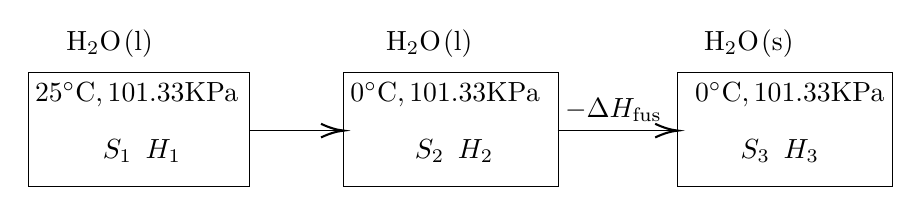
\begin{tikzpicture}[x=0.75pt,y=0.75pt,yscale=-1,xscale=1]
%uncomment if require: \path (0,310); %set diagram left start at 0, and has height of 310

%Straight Lines [id:da5288115988393336] 
\draw    (137,159) -- (180,159) ;
\draw [shift={(182,159)}, rotate = 180] [color={rgb, 255:red, 0; green, 0; blue, 0 }  ][line width=0.75]    (10.93,-3.29) .. controls (6.95,-1.4) and (3.31,-0.3) .. (0,0) .. controls (3.31,0.3) and (6.95,1.4) .. (10.93,3.29)   ;
%Shape: Rectangle [id:dp03627693769346263] 
\draw   (30,131) -- (136.68,131) -- (136.68,186) -- (30,186) -- cycle ;
%Shape: Rectangle [id:dp8461863478385299] 
\draw   (182,131) -- (285.36,131) -- (285.36,186) -- (182,186) -- cycle ;
%Straight Lines [id:da5070236246637718] 
\draw    (285,159) -- (341,159) ;
\draw [shift={(343,159)}, rotate = 180] [color={rgb, 255:red, 0; green, 0; blue, 0 }  ][line width=0.75]    (10.93,-3.29) .. controls (6.95,-1.4) and (3.31,-0.3) .. (0,0) .. controls (3.31,0.3) and (6.95,1.4) .. (10.93,3.29)   ;
%Shape: Rectangle [id:dp9622405190082797] 
\draw   (343,131) -- (446.36,131) -- (446.36,186) -- (343,186) -- cycle ;

% Text Node
\draw (32,134.4) node [anchor=north west][inner sep=0.75pt]    {$25\sssd,101.33\ce{KPa}$};
% Text Node
\draw (184,134.4) node [anchor=north west][inner sep=0.75pt]    {$0\sssd,101.33\ce{KPa}$};
% Text Node
\draw (350,134.4) node [anchor=north west][inner sep=0.75pt]    {$0\sssd,101.33\ce{KPa}$};
% Text Node
\draw (69.22,125) node [anchor=south] [inner sep=0.75pt]  {$\ce{H2O(l)}$};
% Text Node
\draw (223.22,125) node [anchor=south] [inner sep=0.75pt]    {$\ce{H2O(l)}$};
% Text Node
\draw (377.22,125) node [anchor=south] [inner sep=0.75pt]    {$\ce{H2O(s)}$};
% Text Node
\draw (81.34,161.9) node [anchor=north east] [inner sep=0.75pt]    {$S_{1}$};
% Text Node
\draw (85.34,161.9) node [anchor=north west][inner sep=0.75pt]    {$H_{1}$};
% Text Node
\draw (231.68,161.9) node [anchor=north east] [inner sep=0.75pt]    {$S_{2}$};
% Text Node
\draw (235.68,161.9) node [anchor=north west][inner sep=0.75pt]    {$H_{2}$};
% Text Node
\draw (388.68,161.9) node [anchor=north east] [inner sep=0.75pt]    {$S_{3}$};
% Text Node
\draw (392.68,161.9) node [anchor=north west][inner sep=0.75pt]    {$H_{3}$};
% Text Node
\draw (287.36,142.4) node [anchor=north west][inner sep=0.75pt]    {$-\Delta H_{\ce{fus}}$};


\end{tikzpicture}
	\end{center}
	由于在$0\sssd,101.33\ce{KPa}$下,液态水的焓和熵都规定为0,所以:$H_{2} = ,S_{2} = 0$。
	此时整个过程的总焓变为:
	\begin{equation*}
		\Delta H = H_{3} - H_{1} = (H_{3}-H_{2})+(H_{2}-H_{1})  = -\Delta H_{\ce{fus}} + (0-H_{1}) = -334.7-104.89\hdw =-439.59\hdw
	\end{equation*}
	由于相变是恒压过程,则总熵变为:
	\begin{equation*}
		\Delta S = S_{3}-S_{1} = \dfrac{H_{2}-H_{3}}{273.15\ce{K}} +0-S_{1} = -\dfrac{ 334.7}{273.15} - 0.3674 \sdw = -1.5927\sdw
	\end{equation*} 
	那么此时理想功为:
	\begin{equation*}
		\begin{aligned}
			W_{\ce{25\sssd,id}} &= \Delta H - T_{0}\Delta S \\
			&=-439.59 -298.15\times     -1.5927 = 35.27      \ \hdw 
		\end{aligned}
	\end{equation*}
	\item 同理,$-25\sssd$下的理想功为:
	\begin{equation*}
		\begin{aligned}
			W_{\ce{-25\sssd,id}} &= \Delta H - T_{1}\Delta S \\
			&=-439.59 -248.15\times     -1.5927 = -44.36     \ \hdw 
		\end{aligned}
	\end{equation*}
	\end{enumerate}
\end{solution}

\begin{problem}试求:
\begin{enumerate}
	\item 流动过程
	\item 非流动过程
\end{enumerate}
中温度为813K、压力为4.052MPa的1kmol 氮气变至373K、1.013MPa可能做的理想功为多少?取环境温度为$T_{0}$=293K, $p_{0}$=0.1013MPa, 氮气的等压热容为:
$$
	(C_{p})_{\ce{N2}} = 27.98+4.271\times 10^{-3}T\quad \ce{kJ}\cdot\ce{kmol}^{-1}\cdot\ce{K}^{-1}
$$
\end{problem}

\begin{solution}
	\begin{enumerate}
		\item 先计算总过程总焓变\footnote{这里小写的焓$h$、熵$s$功$w$都是指比焓、比熵、比功(即每mol为单位)} :
		\begin{equation*}
			\Delta h = \int_{T_{1}}^{T_{2}} (C_{p})_{\ce{N2}}\ce{d} T = \int_{813\ce{K}}^{373\ce{K}}27.98+4.271\times 10^{-3}T\ce{d}T = 13425.6\ce{kJ}\cdot\ce{kmol}^{-1}
		\end{equation*}
		过程总熵变:
		\begin{equation*}
			\Delta s = \int_{T_{1}}^{T_{2}} \dfrac{ (C_{p})_{\ce{N2}}}{T}\ce{d}T-R\ln\dfrac{p_{2}}{p_{1}} = \int_{813\ce{K}}^{373\ce{K}}\dfrac{27.98+4.271\times 10^{-3}T}{T}\ce{d}T-R\ln\dfrac{1.013}{4.052} = -12.15\ce{kJ}\cdot\ce{kmol}^{-1}\cdot\ce{K}^{-1}
		\end{equation*}
		所以,流动过程氮气之理想功为:
		\begin{equation*}
			w_{\text{流动},\ce{id}} = \Delta h - T_{0}\Delta s = 13425.6-293\times (-12.15) \ce{kJ}\cdot\ce{kmol}^{-1} = -9.866\ce{kJ}\cdot\ce{mol}^{-1}
		\end{equation*}
		\begin{equation*}
			W_{\text{流动},\ce{id}}  = w_{\text{流动},\ce{id}}\times n_{\ce{N2}} = -9866\ce{kJ}
		\end{equation*}
		\item 相比流动过程,非流动过程的理想功要复杂,所以从热力学关系式进行推导\footnote{因为量纲一致,这里的$v$也是比体积(摩尔体积),将理想功单独写出。}:
		\begin{equation*}
			\begin{aligned}
				\ce{d}h &= T_{0} \ce{d}s +v\ce{d}p-w_{id}\\
			\end{aligned}
		\end{equation*}
		利用电动力学常用手段进行凑微分,可得:
		\begin{equation*}
			\ce{d} h= T_{0} \ce{d}s +\ce{d}(pv)-w_{id}-p\ce{d}v
		\end{equation*}
		两边同时对始末态积分,则有:
		\begin{equation*}
			h_{2}-h_{1} = T_{0}(s_{2}-s_{1})+(pv)_{2}-(pv)_{1}-w_{id}-p_{0}(v_{2}-v_{1})
		\end{equation*}
	\end{enumerate}
	反解之:
	\begin{equation*}
		\begin{aligned}
			w_{\text{非流动},\ce{id}} &=-( h_{2}-h_{1}) +T_{0}(s_{2}-s_{1})+(pv)_{2}-(pv)_{1}-p_{0}(v_{2}-v_{1})\\
			&=-w_{\text{流动},\ce{id}}+(pv)_{2}-(pv)_{1}-p_{0}(v_{2}-v_{1})\\
			\end{aligned}
	\end{equation*}
	两边同取$n_{\ce{N2}}$,那么
			\begin{equation*}
		\begin{aligned}
		W_{\text{非流动},\ce{id}}&=-W_{\text{流动},\ce{id}}+R(T_{2}-T_{1})-p_{0}R(\dfrac{T_{2}}{p_{2}}-\dfrac{T_{1}}{p_{1}} )\\
			&=9866+8.314\times(373-813)-0.1013\times 8.314(\dfrac{373}{1.013}-\dfrac{813}{4.052}) \ce{kJ}\cdot\ce{mol}^{-1}= 6066.7\ce{kJ}\cdot\ce{mol}^{-1}
		\end{aligned}
	\end{equation*}
		
		
\end{solution}

\begin{problem}
	1$\ce{kg}$甲烷气由 27\ssd  、$9.80\times 10^{4}$Pa绝热压缩到27\ssd  、$6.666\times 10^{6}$Pa,若实际压缩功耗为1021.6kJ,取$T_{0}$为27\ssd 。试求: 
	\begin{enumerate}
		\item 冷凝器需移走的热量
		\item 压缩与冷却过程的损耗功
		\item 该过程的理想功
		\item 该过程的热力学效率
	\end{enumerate}
\end{problem}

\begin{solution}
	查甲烷的热力学数据\footnote{利用数据库\href{http://www.ap1700.com/default.aspx}{http://www.ap1700.com/default.aspx}查得} 可得:压缩前$h_{1} = 914.4525\hdw$,$s_{1} =6.7068\sdw$压缩后$h_{2} = 848.9254\hdw $,$s_{2} = 4.3571\sdw$。
	\begin{enumerate}
		\item 根据能量守恒关系:
		\begin{equation*}
			(h_{2} - h_{1})\times 1\ce{kg}= -65.5271\ce{kJ}= \Delta H = \Delta W + \Delta Q = 1021.6\ce{kJ}+ \Delta Q 
		\end{equation*}
		得到$\Delta Q = -1087.13\ce{kJ}$
		,所以压缩机需要带走的热量为$1087.13\ce{kJ}$
		\item 根据定义:
		\begin{equation*}
			\begin{aligned}
				\Delta W_{\ce{L}} &= T_{0}\Delta S_{\ce{t}} = T_{0}\pqty{\Delta S_{\ce{sys}} + \Delta S_{\ce{sur}}} \\
				&=T_{0}\pqty{1\ce{kg}\times(s_{2}-s_{1})+\dfrac{\Delta Q}{T}}\\
				&= 300.15\times\pqty{1\ce{kg}\times (4.3571-6.7068)  +\dfrac{1087.13}{300.15}} \ce{kJ} = 381.87\ce{kJ}
			\end{aligned}
		\end{equation*}
		于是损耗功为$381.87\ce{kJ}$
		\item 直接带入计算可知:
		\begin{equation*}
			\Delta W_{\ce{id}} = \Delta H - T_{0}\Delta S = -65.5271 -300.15(4.3571-6.7068)\ce{kJ} = 639.74\ce{kJ}
		\end{equation*}
		所以理想功为$W_{\ce{id}} =639.74\ce{kJ} $
		\item 根据定义可知:
		\begin{equation*}
			\eta  = \dfrac{W_{\ce{id}}}{W_{s}}\times 100\% = \dfrac{639.74}{1021.6}\times 100\% = 62.62\%
		\end{equation*}
	\end{enumerate}
\end{solution}

\begin{problem}
	6.0MPa,400\ssd 的过热蒸汽($H_{1}=3174 \hdw,S_{1}=6.535\sdw $)在稳流过程中经透平绝热膨胀到0.004MPa、干度$x=0.9$。(已知0.004 MPa下$H_{\ce{g}}=2554 \hdw ,S_{\ce{g}}=8.4808\sdw , H_{\ce{l}}=120 \hdw , S_{\ce{l}}=0.4177 \sdw$)。$T_{0}=298\ce{K}$。求该过程的$W_{\ce{id}}$、$W_{\ce{ac}}$、$W_{\ce{L}}$及热力学效率$\eta$。
\end{problem}


\begin{solution}
	由于末态为汽液混合物,根据混合规则:
	\begin{equation*}
		H_{2} = xH_{\ce{g}}+(1-x)H_{\ce{l}} = 0.9\times 2554+(1-0.9)\times 120\ \hdw = 2310.6\hdw
	\end{equation*}
	\begin{equation*}
		S_{2} =xS_{\ce{g}}+(1-x)S_{\ce{l}} = 0.9\times 8.4808+(1-0.9)\times 0.4177\ \sdw = 7.6745\sdw
	\end{equation*}
	于是:
	\begin{itemize}
		\item $W_{\ce{ac}} = W_{s} = \Delta H = H_{2} - H_{1} = 2310.6 - 3174\ \hdw =-863.4 \hdw$
		\item $W_{\ce{id}} = \Delta H - T_{0}\Delta S = -863.4-298.15\times (7.6745-6.535)\ \hdw = -1203.1\hdw$
		\item $W_{\ce{L}} =T_{0}\Delta S  = 298.15\times(7.6745-6.535) \ \hdw = 339.74\hdw$
	\end{itemize}
	热力学效率为:
	\begin{equation*}
		\eta = \dfrac{W_{s}}{W_{\ce{id}}} = \dfrac{863.4}{1203.1}\times 100\% = 71.76\%
	\end{equation*}
\end{solution}


\begin{problem}
	某干燥工艺需要用到400K、0.1MPa的干净热空气,燃烧炉产生的热空气规格为600K、0.1MPa,流量为224标准$\ce{L}\cdot \ce{s}^{-1}$,通过换热器将300K、0.1MPa,流量为224标准L的普通空气加热到指定温度。假设燃烧炉空气和普通空气都可视为理想气体,且$C_{p} = \dfrac{7}{2}R \quad (\ce{J}\cdot\ce{mol}^{-1}\cdot\ce{K}^{-1})$,环境温度为300K。求该稳定流动过程的传热速率和熵产生。(标准体积定义:1个标准大气压、0\ssd 下的摩尔体积为22.4L)
\end{problem}

\begin{solution}
	根据题目所言,气体均视作理想气体,那么其摩尔流量均为$V_{s} = \dfrac{224}{22.4}\ce{mol}\cdot\ce{s}^{-1}$,由于是恒压过程,所以对于普通空气有:
	\begin{equation*}
		\Delta h = \int_{T_{1}}^{T_{2}}C_{p}\ce{d}T = \int_{300\ce{K}}^{400\ce{K}}\dfrac{7}{2}R\ce{d}T  = 2909.9\ce{J}\cdot\ce{mol}^{-1}
	\end{equation*}
	根据能量守恒方程,无外做功,那么传热速率为:
	\begin{equation*}
		q = V_{s}\Delta h= 29.099\ce{kJ}\cdot\ce{s}^{-1}
	\end{equation*}
	由于是稳定流动过程,所以熵积累为0,故熵产生为:
	\begin{equation*}
		\Delta S =V_{s}\pqty{ \int_{T_{1}}^{T_{2}}\dfrac{C_{p}}{T}\ce{d}T - \Delta S_{f}} =10\pqty{ \int_{300\ce{K}}^{400\ce{K}}\dfrac{7R}{2T}\ce{d}T -\dfrac{2909.9}{600}} = 35.21\ce{J}\cdot\ce{K}^{-1}\cdot\ce{s}^{-1}
	\end{equation*}
\end{solution}
\begin{tip}
	稍微有点儿混乱,整理一下:
	\begin{center}
		

\tikzset{every picture/.style={line width=0.75pt}} %set default line width to 0.75pt        

\begin{tikzpicture}[x=0.75pt,y=0.75pt,yscale=-1,xscale=1]
%uncomment if require: \path (0,300); %set diagram left start at 0, and has height of 300

%Shape: Rectangle [id:dp9510552442572187] 
\draw   (211,90) -- (415,90) -- (415,150) -- (211,150) -- cycle ;
%Straight Lines [id:da3357173678139078] 
\draw    (100,121) -- (209,121) ;
\draw [shift={(211,121)}, rotate = 180] [color={rgb, 255:red, 0; green, 0; blue, 0 }  ][line width=0.75]    (10.93,-3.29) .. controls (6.95,-1.4) and (3.31,-0.3) .. (0,0) .. controls (3.31,0.3) and (6.95,1.4) .. (10.93,3.29)   ;
%Straight Lines [id:da11165088187336059] 
\draw    (526,120) -- (417,120) ;
\draw [shift={(415,120)}, rotate = 360] [color={rgb, 255:red, 0; green, 0; blue, 0 }  ][line width=0.75]    (10.93,-3.29) .. controls (6.95,-1.4) and (3.31,-0.3) .. (0,0) .. controls (3.31,0.3) and (6.95,1.4) .. (10.93,3.29)   ;
%Straight Lines [id:da5023397585236646] 
\draw    (311,90) -- (311,34) ;
\draw [shift={(311,32)}, rotate = 90] [color={rgb, 255:red, 0; green, 0; blue, 0 }  ][line width=0.75]    (10.93,-3.29) .. controls (6.95,-1.4) and (3.31,-0.3) .. (0,0) .. controls (3.31,0.3) and (6.95,1.4) .. (10.93,3.29)   ;
%Straight Lines [id:da2607991266926344] 
\draw    (310,150) -- (310,208) ;
\draw [shift={(310,210)}, rotate = 270] [color={rgb, 255:red, 0; green, 0; blue, 0 }  ][line width=0.75]    (10.93,-3.29) .. controls (6.95,-1.4) and (3.31,-0.3) .. (0,0) .. controls (3.31,0.3) and (6.95,1.4) .. (10.93,3.29)   ;

% Text Node
\draw (155.5,117.6) node [anchor=south] [inner sep=0.75pt]    {$ \begin{array}{l}
{\textstyle n_{1} =10\ce{mol}\cdot\ce{s}^{-1}}\\
{\textstyle T_{1}=600\ce{K}}
\end{array}$};
% Text Node
\draw (470.5,116.6) node [anchor=south] [inner sep=0.75pt]    {$ \begin{array}{l}
{\textstyle n_{2} =10\ce{mol}\cdot\ce{s}^{-1}}\\
{\textstyle T_{2}=300\ce{K}}
\end{array}$};
% Text Node
\draw (309,32) node [anchor=east] [inner sep=0.75pt]    {$ \begin{array}{l}
{\textstyle n =20\ce{mol}\cdot\ce{s}^{-1}}\\
{\textstyle T=400\ce{K}}
\end{array}$};
% Text Node
\draw (312,213.4) node [anchor=north west][inner sep=0.75pt]    {$q$};
% Text Node
\draw (313,120) node   [align=left] {系统};


\end{tikzpicture}
	\end{center}
	这里的熵产$\Delta S_{\ce{g}}$这样计算:
	\begin{equation*}
		\begin{aligned}
			\Delta S_{\ce{g}} &= \sum_{j}(m_{j}S_{j})-\sum_{i}(m_{i}S_{i})-\Delta S_{\ce{f}}\\
			&=(n_{1}+n_{2})S - (n_{1}S_{1}+n_{2}S_{2})+\dfrac{q}{T_{0}}\\
			&=n_{2}(S-S_{2})+n_{1}(S-S_{1})+\dfrac{q}{T_{0}}\\
			&=n_{2}C_{p}\ln\dfrac{T}{T_{2}}+n_{1}C_{p}\ln\dfrac{T}{T_{1}}+\dfrac{q}{T_{0}}\\
			&=10\times \dfrac{7}{2}\times 8.314\times(\ln\dfrac{400}{600}+\ln\dfrac{400}{300})+\dfrac{29099}{300}\ \ce{J}\cdot\ce{K}^{-1}\cdot\ce{s}^{-1}\\
			&=62.72\ce{J}\cdot\ce{K}^{-1}\cdot\ce{s}^{-1}
		\end{aligned}
	\end{equation*}
	这里上面绿色做法错误的原因是因为两个都属于原来的熵,非相减关系,所以末态的熵是叠加而不是相约。
\end{tip}


\chapter{2022年5月19日 \quad 雷阵雨}
\begin{problem}
	某合成氨厂甲烷蒸汽转化工段转化气量为$5160\ce{Nm}^{3}\cdot\ce{t}^{-1}\ce{NH3}$,因工艺需要将其温度从1000\ssd 降至370\ssd 。通过废热锅炉机组回收余热,已知通过蒸汽透平回收到的实际功为$439\ce{kWh}\cdot\ce{t}^{-1}\ce{NH3}$。试求:
	\begin{enumerate}
		\item 转化气降温过程的理想功;	
		\item 余热利用动力装置的热效率;
		\item 此余热利用过程的热力学效率。
	\end{enumerate}
已知大气温度为25\ssd ,设转化气降温过程压力不变,在$370\sim 1000\sssd$温度范围内平均等压热容为$\overline{C}_{p} = 36\ce{kJ}\cdot\ce{kmol}^{-1}\cdot\ce{K}^{-1}$,废热锅炉和透平的热损失可忽略不计,透平乏汽直接排入大气。
\end{problem}

\begin{solution}
	以$1\ce{t}\ce{NH3}$作为衡算基准:
	
	那么$1\ce{t}\ \ce{NH3}$的物质的量为$n = \dfrac{5160}{22.4\times 10^{3}}\ce{mol} = 230.357\ce{kmol}$
	\begin{enumerate}
		\item 根据理想功的定义式:
		\begin{equation*}
			\begin{aligned}
				W_{\ce{id}} &= \Delta H-T_{0}\Delta S = n\pqty{\int_{1273.15\ce{K}}^{643.15\ce{K}}C_{p}\ce{d}T - T_{0}\ce{K}\times\int_{1273.15\ce{K}}^{643.15\ce{K}}\dfrac{C_{p}}{T}\ce{d}T}\\
				&=230.357\pqty{\int_{1273.15}^{643.15}36\ce{d}T - 298.15\ce{K}\times\int_{1273.15}^{643.15}\dfrac{36}{T}\ce{d}T} \  \ce{kJ}\\
				&=-982.43\ce{kWh}
			\end{aligned}
		\end{equation*}
		\item 恒压过程有:
		\begin{equation*}
			\begin{aligned}
				Q &= \Delta H = n \int_{1273.15\ce{K}}^{643.15\ce{K}}C_{p}\ce{d}T\\
				&=230.357\int_{1273.15\ce{K}}^{643.15\ce{K}}36\ce{d}T\  \ce{kJ}\\
				&=-1451.25\ce{kWh}
			\end{aligned}
		\end{equation*}
		所以热效率为:
		\begin{equation*}
			\eta_{heat} = \dfrac{W_{\ce{s}}}{Q} = \dfrac{439}{1451.25}\times 100\% = 30.25\% 
		\end{equation*}
		\item 热力学效率为:
		\begin{equation*}
			\eta = \dfrac{W_{\ce{s}}}{W_{\ce{id}}} = \dfrac{439}{982.43}\times 100\% = 44.69\%
		\end{equation*}
	\end{enumerate}
	
\end{solution}


\begin{problem}
	某工厂有两种余热可利用。一种是高温烟道气,主要成分是$\ce{CO2}$、$\ce{N2}$和水蒸气,流量为$500\ce{kg}\cdot\ce{h}^{-1}$,温度为800\ssd ,其平均等压热容为$0.8\ce{kJ}\cdot\ce{kg}^{-1}\cdot\ce{K}^{-1}$;另一种是低温排水,流量为$1348\ce{kg}\cdot\ce{h}^{-1}$,温度为80\ssd,其平均等压热容为$4.18\ce{kJ}\cdot\ce{kg}^{-1}\cdot\ce{K}^{-1}$。环境温度$T_{0}=25\sssd$,求两种余热的有效能各为多少。
\end{problem}

\begin{solution}
	直接带入公式:
	\begin{enumerate}
		\item 对于高温烟道气:
		\begin{equation*}
			\begin{aligned}
				E_{\ce{x,\text{高温烟道气}}} &= m\pqty{\int_{298.15\ce{K}}^{1073.15\ce{K}} C_{p}\ce{d}T - T_{0}\int_{298.15\ce{K}}^{1073.15\ce{K}} \dfrac{C_{p}}{T}\ce{d}T}\\
				& =500\pqty{\int_{298.15}^{1073.15} 0.8\ce{d}T - 298.15\int_{298.15}^{1073.15} \dfrac{0.8}{T}\ce{d}T}\ \ce{kJ}\cdot\ce{h}^{-1}\\
				&=157257\ce{kJ}\cdot\ce{h}^{-1}
			\end{aligned}		
			\end{equation*}
		\item 对于低温排水:
		\begin{equation*}
			\begin{aligned}
				E_{\ce{x,\text{低温排水}}} &= m\pqty{\int_{298.15\ce{K}}^{353.15\ce{K}} C_{p}\ce{d}T - T_{0}\int_{298.15\ce{K}}^{353.15\ce{K}} \dfrac{C_{p}}{T}\ce{d}T}\\
				& =1348\pqty{\int_{298.15}^{353.15} 4.18\ce{d}T - 298.15\int_{298.15}^{353.15} \dfrac{4.18}{T}\ce{d}T}\ \ce{kJ}\cdot\ce{h}^{-1}\\
				&=25493\ce{kJ}\cdot\ce{h}^{-1}
			\end{aligned}		
			\end{equation*}
	\end{enumerate}
\end{solution}

\begin{problem}
	某工厂有一输送90\ssd 热水的管道,由于保温不良,到使用单位,水温降至70\ssd ,试计算热水由于散热而引起的有效能损失。设大气温度为298K。已知水的恒压热容为$4186.8\ce{J}\cdot\ce{kg}^{-1}\cdot\ce{K}^{-1}$。
\end{problem}

\begin{solution}
	有效能损失指有效能之差:
	\begin{equation*}
			\begin{aligned}
				E_{\ce{x},\ce{L}} &= \int_{343.15\ce{K}}^{363.15\ce{K}} C_{p}\ce{d}T - T_{0}\int_{343.15\ce{K}}^{363.15\ce{K}} \dfrac{C_{p}}{T}\ce{d}T\\
				& =\int_{343.15}^{363.15} 4186.8\ce{d}T - 298\int_{343.15}^{363.15} \dfrac{4186.8}{T}\ce{d}T\ \ce{J}\cdot\ce{kg}^{-1}\\
				&=13057.8\ce{J}\cdot\ce{kg}^{-1}
			\end{aligned}		
			\end{equation*}
\end{solution}




\begin{problem}
	将0.1MPa、127\ssd 的1kg空气可逆定压加热到427\ssd.试求:
	\begin{enumerate}
		\item 加热量中的有效能和无效能(热量由热源的显热供给,因此热源的温度是变化的)。
		\item 如果同样的加热量,由500\ssd 的恒温热源放出,则加热量中的有效能和无效能又为多少?
	\end{enumerate}
设环境温度为25\ssd ,空气的平均等压热容为$1.004\ce{kJ}\cdot\ce{kg}^{-1}\cdot\ce{K}^{-1}$
\end{problem}

\begin{solution}
	\begin{enumerate}
		\item 空气获得的热量为:
		\begin{equation*}
			Q = \Delta H = \int_{400.15}^{700.15}1.004\ce{d}T \ \ce{kJ}\cdot\ce{kg}^{-1}=301.2\ce{kJ}\cdot\ce{kg}^{-1}
		\end{equation*}
		由于此过程为可逆过程,则:
		\begin{equation*}
			\Delta S = \int_{400.15}^{700.15}\dfrac{1.004}{T}\ce{d}T = 0.5617\ce{kJ}\cdot\ce{kg}^{-1}\cdot\ce{K}^{-1}
		\end{equation*}
		于是无效能、有效能分别为:
		\begin{equation*}
			\begin{aligned}
				A_{\ce{NQ}} &= T_{0}\Delta S = 298.15 \times 0.5617\ce{kJ}\cdot\ce{kg}^{-1} = 167.47\ce{kJ}\cdot\ce{kg}^{-1}\\
				E_{\ce{x},Q} &= Q - A_{\ce{NQ}} = 301.2-167.47\ \ce{kJ}\cdot\ce{kg}^{-1} = 133.73\ce{kJ}\cdot\ce{kg}^{-1}
			\end{aligned}
		\end{equation*}
		\item 由于获得同样的加热量,那么:
		\begin{equation*}
			\begin{aligned}
				E_{\ce{x},Q} &= Q\pqty{1-\dfrac{T_{0}}{773.15\ce{K}}} = 301.2\pqty{1-\dfrac{298.15}{773.15}} \ \ce{kJ}\cdot\ce{kg}^{-1} =185.1\ce{kJ}\cdot\ce{kg}^{-1}\\
				A_{\ce{NQ}} &= Q - E_{\ce{x},Q} = 301.2-185.1\ \ce{kJ}\cdot\ce{kg}^{-1} =116.1\ce{kJ}\cdot\ce{kg}^{-1}
			\end{aligned}
		\end{equation*}
	\end{enumerate}
\end{solution}




\begin{problem}
	如下页图所示,裂解气在中冷塔中分离,塔的操作压力为3.444MPa,液态烃(由C2、C3、C4等组成)由塔底进入再沸器,其温度为45\ssd ;经0.197MPa的饱和蒸汽加热蒸发回到塔内。求加热前后液态烃、水蒸气的有效能变化及损失功。
	
	
	已知:再沸器中冷凝水为40\ssd ,大气的温度为20\ssd ,液态烃在45\ssd 、3.444MPa下的汽化热为293$\ce{kJ}\cdot\ce{kg}$,汽化熵为$0.921\sdw$;0.197MPa的饱和水蒸气饱和温度为119.6\ssd,$H_{\text{汽}} = 2706 \hdw$,$S_{\text{汽}} = 7.133 \sdw$,40\ssd 的饱和水,$H_{\text{水}} = 167.4\hdw$,$S_{\text{水}} = 0.572 \sdw$。
	
	\begin{center}
		

\tikzset{every picture/.style={line width=0.75pt}} %set default line width to 0.75pt        

\tikzset{every picture/.style={line width=0.75pt}} %set default line width to 0.75pt        

\begin{tikzpicture}[x=0.75pt,y=0.75pt,yscale=-1,xscale=1]
%uncomment if require: \path (0,300); %set diagram left start at 0, and has height of 300

%Shape: Arc [id:dp3840464663142502] 
\draw  [draw opacity=0] (216,86) .. controls (216,86) and (216,86) .. (216,86) .. controls (216,69.43) and (229.43,56) .. (246,56) .. controls (262.57,56) and (276,69.43) .. (276,86) -- (246,86) -- cycle ; \draw   (216,86) .. controls (216,86) and (216,86) .. (216,86) .. controls (216,69.43) and (229.43,56) .. (246,56) .. controls (262.57,56) and (276,69.43) .. (276,86) ;  
%Shape: Arc [id:dp655605171214221] 
\draw  [draw opacity=0] (276,199) .. controls (276,199) and (276,199) .. (276,199) .. controls (276,215.57) and (262.57,229) .. (246,229) .. controls (229.43,229) and (216,215.57) .. (216,199) -- (246,199) -- cycle ; \draw   (276,199) .. controls (276,199) and (276,199) .. (276,199) .. controls (276,215.57) and (262.57,229) .. (246,229) .. controls (229.43,229) and (216,215.57) .. (216,199) ;  
%Straight Lines [id:da25872901779383617] 
\draw    (216,86) -- (216,199) ;
%Straight Lines [id:da8331667644265399] 
\draw    (276,86) -- (276,199) ;
%Straight Lines [id:da509297190416131] 
\draw    (140,142.5) -- (214,142.5) ;
\draw [shift={(216,142.5)}, rotate = 180] [color={rgb, 255:red, 0; green, 0; blue, 0 }  ][line width=0.75]    (10.93,-3.29) .. controls (6.95,-1.4) and (3.31,-0.3) .. (0,0) .. controls (3.31,0.3) and (6.95,1.4) .. (10.93,3.29)   ;
%Straight Lines [id:da8074468579142453] 
\draw    (245,27) -- (245,56) ;
%Straight Lines [id:da17165005886578588] 
\draw    (245,27) -- (312,27) ;
%Straight Lines [id:da7267271386651479] 
\draw    (312,27) -- (312,41) ;
%Shape: Circle [id:dp5245459252187876] 
\draw   (302.5,50.5) .. controls (302.5,45.25) and (306.75,41) .. (312,41) .. controls (317.25,41) and (321.5,45.25) .. (321.5,50.5) .. controls (321.5,55.75) and (317.25,60) .. (312,60) .. controls (306.75,60) and (302.5,55.75) .. (302.5,50.5) -- cycle ;
%Straight Lines [id:da8060322654834631] 
\draw    (312,60) -- (312,83) ;
%Straight Lines [id:da9844835944232198] 
\draw    (312,83) -- (344,83) ;
\draw [shift={(346,83)}, rotate = 180] [color={rgb, 255:red, 0; green, 0; blue, 0 }  ][line width=0.75]    (10.93,-3.29) .. controls (6.95,-1.4) and (3.31,-0.3) .. (0,0) .. controls (3.31,0.3) and (6.95,1.4) .. (10.93,3.29)   ;
%Straight Lines [id:da512642037445675] 
\draw    (312,83) -- (278,83) ;
\draw [shift={(276,83)}, rotate = 360] [color={rgb, 255:red, 0; green, 0; blue, 0 }  ][line width=0.75]    (10.93,-3.29) .. controls (6.95,-1.4) and (3.31,-0.3) .. (0,0) .. controls (3.31,0.3) and (6.95,1.4) .. (10.93,3.29)   ;
%Straight Lines [id:da4082349727551444] 
\draw    (298,63) -- (329.47,36.29) ;
\draw [shift={(331,35)}, rotate = 139.69] [color={rgb, 255:red, 0; green, 0; blue, 0 }  ][line width=0.75]    (10.93,-3.29) .. controls (6.95,-1.4) and (3.31,-0.3) .. (0,0) .. controls (3.31,0.3) and (6.95,1.4) .. (10.93,3.29)   ;
%Straight Lines [id:da14770923384945922] 
\draw    (246,229) -- (246,262) ;
\draw [shift={(246,264)}, rotate = 270] [color={rgb, 255:red, 0; green, 0; blue, 0 }  ][line width=0.75]    (10.93,-3.29) .. controls (6.95,-1.4) and (3.31,-0.3) .. (0,0) .. controls (3.31,0.3) and (6.95,1.4) .. (10.93,3.29)   ;
%Straight Lines [id:da8391735833019287] 
\draw    (337,264) -- (337,224) ;
\draw [shift={(337,222)}, rotate = 90] [color={rgb, 255:red, 0; green, 0; blue, 0 }  ][line width=0.75]    (10.93,-3.29) .. controls (6.95,-1.4) and (3.31,-0.3) .. (0,0) .. controls (3.31,0.3) and (6.95,1.4) .. (10.93,3.29)   ;
%Shape: Rectangle [id:dp3943549095558172] 
\draw   (322,170) -- (352,170) -- (352,221) -- (322,221) -- cycle ;
%Straight Lines [id:da03802845565779167] 
\draw    (337,142.5) -- (337,170) ;
%Straight Lines [id:da02519192784250479] 
\draw    (337,142.5) -- (278,142.5) ;
\draw [shift={(276,142.5)}, rotate = 360] [color={rgb, 255:red, 0; green, 0; blue, 0 }  ][line width=0.75]    (10.93,-3.29) .. controls (6.95,-1.4) and (3.31,-0.3) .. (0,0) .. controls (3.31,0.3) and (6.95,1.4) .. (10.93,3.29)   ;
%Straight Lines [id:da10937871036315072] 
\draw    (246,264) -- (337,264) ;
%Straight Lines [id:da27268306473183057] 
\draw    (337,179) .. controls (338.67,180.67) and (338.67,182.33) .. (337,184) .. controls (335.33,185.67) and (335.33,187.33) .. (337,189) .. controls (338.67,190.67) and (338.67,192.33) .. (337,194) .. controls (335.33,195.67) and (335.33,197.33) .. (337,199) .. controls (338.67,200.67) and (338.67,202.33) .. (337,204) .. controls (335.33,205.67) and (335.33,207.33) .. (337,209) -- (337,212) -- (337,212) ;
%Straight Lines [id:da4425351572586327] 
\draw [color={rgb, 255:red, 0; green, 0; blue, 0 }  ,draw opacity=1 ]   (399,179) -- (339,179) ;
\draw [shift={(337,179)}, rotate = 360] [color={rgb, 255:red, 0; green, 0; blue, 0 }  ,draw opacity=1 ][line width=0.75]    (10.93,-3.29) .. controls (6.95,-1.4) and (3.31,-0.3) .. (0,0) .. controls (3.31,0.3) and (6.95,1.4) .. (10.93,3.29)   ;
%Shape: Rectangle [id:dp3714510248196643] 
\draw  [color={rgb, 255:red, 208; green, 2; blue, 27 }  ,draw opacity=1 ][dash pattern={on 0.84pt off 2.51pt}] (316,119) -- (387,119) -- (387,278) -- (316,278) -- cycle ;
%Straight Lines [id:da5909814211818274] 
\draw [color={rgb, 255:red, 0; green, 0; blue, 0 }  ,draw opacity=1 ]   (397,212) -- (337,212) ;
\draw [shift={(399,212)}, rotate = 180] [color={rgb, 255:red, 0; green, 0; blue, 0 }  ,draw opacity=1 ][line width=0.75]    (10.93,-3.29) .. controls (6.95,-1.4) and (3.31,-0.3) .. (0,0) .. controls (3.31,0.3) and (6.95,1.4) .. (10.93,3.29)   ;

% Text Node
\draw (245.5,143.5) node   [align=left] {中\\冷\\塔};
% Text Node
\draw (278,139.1) node [anchor=south west] [inner sep=0.75pt]    {$气烃$};
% Text Node
\draw (248,267.4) node [anchor=north west][inner sep=0.75pt]    {$液烃$};
% Text Node
\draw (278,145.9) node [anchor=north west][inner sep=0.75pt]    {$45\sssd$};
% Text Node
\draw (248,260.6) node [anchor=south west] [inner sep=0.75pt]    {$45\sssd$};
% Text Node
\draw (389,115.6) node [anchor=south west] [inner sep=0.75pt]  [color={rgb, 255:red, 208; green, 2; blue, 27 }  ,opacity=1 ]  {$318\ce{K}$};
% Text Node
\draw (373,175.6) node [anchor=south west] [inner sep=0.75pt]    {$\text{饱和蒸汽},\ 0.1695,\ 119.6\sssd$};
% Text Node
\draw (373,215.4) node [anchor=north west][inner sep=0.75pt]    {$\text{冷凝水},\ 40\sssd$};
% Text Node
\draw (300,165) node [anchor=north west][inner sep=0.75pt]   [align=left] {再\\沸\\器};

\end{tikzpicture}
	\end{center}
\end{problem}



\begin{solution}
	以1kg水蒸气作为衡算基准,忽略热损失,则根据能量守恒方程:
	\begin{equation*}
		Q_{\ce{H}} = Q_{\ce{L}} 
	\end{equation*}
	把各项表达出来即:
	\begin{equation*}
		1\ce{kg}\cdot (H_{\text{汽}}- H_{\text{水}}) = mH_{\ce{Vap}} 
	\end{equation*}
	其中$m$是1kg水蒸汽可以蒸发的液态烃的质量为:$m = \dfrac{2706-167.4}{293} \ce{kg}  = 8.664\ce{kg}$
	
	这样$8.664\ce{kg}$液态烃气化所对应的有效能为:
	\begin{equation*}
		E_{\ce{x},\text{烃}} = m(\Delta H_{\text{烃}} - T_{0}\Delta S_{\text{烃}}) = 8.664(293-293.15\times 0.921) \  \ce{kJ}= 199.3\ce{kJ}
	\end{equation*}
	1kg水的有效能:
	\begin{equation*}
		E_{\ce{x},\text{水}} =  m(\Delta H_{\text{水}} - T_{0}\Delta S_{\text{水}})  = (167.4-2706)-293.15\times (0.572-7.133) \ \ce{kJ} = -615.4\ce{kJ}
	\end{equation*}
	损失功为:
	\begin{equation*}
		W_{\ce{L}} = T_{0}\Delta S = 293.15(8.664\times 0.921 + (0.572-7.133))\ \ce{kJ} = 415.8\ce{kJ}
	\end{equation*}
\end{solution}





\begin{problem}
	有一逆流式换热器,利用废气加热空气。空气由$10^{5}\ce{Pa}$、293K加热到398K,空气的流量为$1.5\ce{kg}\cdot\ce{s}^{-1}$;而废气从$1.3\times 10^{5}\ce{Pa}$、523K冷却到368K。空气的等压热容为$1.04\ce{kJ}\cdot\ce{kg}^{-1}\cdot\ce{K}^{-1}$,废气的等压热容为$0.84\ce{kJ}\cdot\ce{kg}^{-1}\cdot\ce{K}^{-1}$。假定空气与废气通过换热器的压力与动能变化可忽略不计,而且换热器与环境无热量交换,环境状态为$10^{5}\ce{Pa}$、293K。试求:
\begin{enumerate}
	\item 换热器中不可逆传热的有效能损失;
	\item 换热器的有效能效率。
\end{enumerate}	
\begin{center}
\tikzset{every picture/.style={line width=0.75pt}} %set default line width to 0.75pt        

\begin{tikzpicture}[x=0.75pt,y=0.75pt,yscale=-1,xscale=1]
%uncomment if require: \path (0,300); %set diagram left start at 0, and has height of 300

%Shape: Rectangle [id:dp36210968393390663] 
\draw   (220,111) -- (398,111) -- (398,180) -- (220,180) -- cycle ;
%Straight Lines [id:da2357595895572666] 
\draw [color={rgb, 255:red, 74; green, 144; blue, 226 }  ,draw opacity=1 ]   (170,130) -- (448,130) ;
\draw [shift={(450,130)}, rotate = 180] [color={rgb, 255:red, 74; green, 144; blue, 226 }  ,draw opacity=1 ][line width=0.75]    (10.93,-3.29) .. controls (6.95,-1.4) and (3.31,-0.3) .. (0,0) .. controls (3.31,0.3) and (6.95,1.4) .. (10.93,3.29)   ;
%Straight Lines [id:da08782559194157691] 
\draw [color={rgb, 255:red, 208; green, 2; blue, 27 }  ,draw opacity=1 ]   (450,160) -- (172,160) ;
\draw [shift={(170,160)}, rotate = 360] [color={rgb, 255:red, 208; green, 2; blue, 27 }  ,draw opacity=1 ][line width=0.75]    (10.93,-3.29) .. controls (6.95,-1.4) and (3.31,-0.3) .. (0,0) .. controls (3.31,0.3) and (6.95,1.4) .. (10.93,3.29)   ;


% Text Node
\draw (309,145.5) node   [align=left] {逆流式换热器};
% Text Node
\draw (218,107.6) node [anchor=south east] [inner sep=0.75pt]    {$m_{a}$};
% Text Node
\draw (400,183.4) node [anchor=north west][inner sep=0.75pt]    {$m_{b}$};
% Text Node
\draw (168,126.6) node [anchor=south east] [inner sep=0.75pt]    {空气$p_{1} ,t_{1} ,E_{\ce{x1}}$};
% Text Node
\draw (452,126.6) node [anchor=south west] [inner sep=0.75pt]    {$p_{1},t_{2},E_{\ce{x2}}$};
% Text Node
\draw (452,163.4) node [anchor=north west][inner sep=0.75pt]    {$p_{3},t_{3},E_{\ce{x3}}$废气};
% Text Node
\draw (168,163.4) node [anchor=north east] [inner sep=0.75pt]    {$p_{3},t_{4},E_{\ce{x4}}$};


\end{tikzpicture}
	\end{center}
\end{problem}

\begin{solution}
\begin{enumerate}
	\item 根据能量守恒方程:
	\begin{equation*}
		\begin{aligned}
			m_{a} C_{p,\text{空气}}(t_{2}-t_{1}) &= m_{b}C_{p,\text{废气}}(t_{3} - t_{4})\\
			1.5\times 1.04(398-293) &= \dfrac{m_{b}}{\ce{kg}\cdot\ce{s}^{-1}} \times 0.84 (523-368)\\
		\end{aligned}
	\end{equation*}
	解得$m_{b} = 1.258\ce{kg}\cdot\ce{s}^{-1}$。因为空气废气压力动能变化忽略不计,与环境无热交换,因此换热器中不可逆传热的有效能损失为:
	\begin{equation*}
		\begin{aligned}
			E_{\ce{L}} &= m_{a}E_{x1}+m_{b}E_{x3}-m_{a}E_{\ce{x2}}-m_{b}E_{\ce{x4}}\\
			&=m_{a}(\Delta_{2}^{1}H_{\text{空气}}-T_{0}\Delta_{2}^{1}S_{\text{空气}}) + m_{b}(\Delta_{4}^{3}H_{\text{废气}}-T_{0}\Delta_{3}^{4}S_{\text{废气}})\\
			&=m_{a}\pqty{\int_{t_{2}}^{t_{1}}C_{\text{空气}}\ce{d}T - T_{0}\int_{t_{2}}^{t_{1}}\dfrac{C_{\text{空气}}}{T}\ce{d}T} + m_{b}\pqty{\int_{t_{4}}^{t_{3}}C_{\text{废气}}\ce{d}T - T_{0}\int_{t_{4}}^{t_{3}}\dfrac{C_{\text{废气}}}{T}\ce{d}T}\\
			&=1.5\pqty{\int_{398}^{293}1.04\ce{d}T - 293\int_{398}^{293}\dfrac{1.04}{T}\ce{d}T}+1.258\pqty{\int_{368}^{523}0.84\ce{d}T - 293\int_{368}^{523}\dfrac{0.84}{T}\ce{d}T} \ce{kJ}\cdot\ce{s}^{-1}\\
			&=31.16 \ce{kJ}\cdot\ce{s}^{-1}\\
		\end{aligned}
	\end{equation*}
	\item 换热器的有效能效率为:
	\begin{equation*}
		\begin{aligned}
			\eta &= \left| \dfrac{m_{b}(\Delta_{4}^{3}H_{\text{废气}}-T_{0}\Delta_{3}^{4}S_{\text{废气}})}{m_{a}(\Delta_{2}^{1}H_{\text{空气}}-T_{0}\Delta_{2}^{1}S_{\text{空气}})}\right|\times 100\%\\
			&=\left|\dfrac{m_{b}\pqty{\displaystyle\int_{t_{4}}^{t_{3}}C_{\text{废气}}\ce{d}T - T_{0}\displaystyle\int_{t_{4}}^{t_{3}}\dfrac{C_{\text{废气}}}{T}\ce{d}T}}{m_{a}\pqty{\displaystyle\int_{t_{2}}^{t_{1}}C_{\text{空气}}\ce{d}T - T_{0}\displaystyle\int_{t_{2}}^{t_{1}}\dfrac{C_{\text{空气}}}{T}\ce{d}T}}\right|\times 100\%\\
			&=\left|\dfrac{1.258\pqty{\displaystyle\int_{368}^{523}0.84\ce{d}T - 293\displaystyle\int_{368}^{523}\dfrac{0.84}{T}\ce{d}T}}{1.5\pqty{\displaystyle\int_{398}^{293}1.04\ce{d}T - 293\displaystyle\int_{398}^{293}\dfrac{1.04}{T}\ce{d}T}}\right|\times 100\%\\
			&=\dfrac{23.80}{54.96}\times 100\% = 43.30\%
		\end{aligned}
	\end{equation*}
	\end{enumerate}
\end{solution}






\begin{problem}
	某一理想的Rankine(朗肯)循环,锅炉的压力为4.0MPa,冷凝器的压力为0.005MPa,冷凝温度为32.56\ssd ,将以下两种条件时的Rankine循环示意的表示在$T-S$图上。
	\begin{enumerate}
		\item 如果进入气轮机的蒸气是饱和蒸气;
		\item 如果进入气轮机的是温度为440\ssd 的过热蒸气。
	\end{enumerate}
\end{problem}


\begin{solution}
	\begin{enumerate}
		\item 如果进入气轮机的蒸气是饱和蒸气,那么Rankine循环示意如下:
		\begin{center}
			

\tikzset{every picture/.style={line width=0.75pt}} %set default line width to 0.75pt        

\begin{tikzpicture}[x=0.75pt,y=0.75pt,yscale=-1,xscale=1]
%uncomment if require: \path (0,310); %set diagram left start at 0, and has height of 310

%Straight Lines [id:da2974359633226489] 
\draw    (108,227) -- (371,227) ;
\draw [shift={(373,227)}, rotate = 180] [color={rgb, 255:red, 0; green, 0; blue, 0 }  ][line width=0.75]    (10.93,-3.29) .. controls (6.95,-1.4) and (3.31,-0.3) .. (0,0) .. controls (3.31,0.3) and (6.95,1.4) .. (10.93,3.29)   ;
%Straight Lines [id:da878410515074896] 
\draw    (136,249) -- (136,21) ;
\draw [shift={(136,19)}, rotate = 90] [color={rgb, 255:red, 0; green, 0; blue, 0 }  ][line width=0.75]    (10.93,-3.29) .. controls (6.95,-1.4) and (3.31,-0.3) .. (0,0) .. controls (3.31,0.3) and (6.95,1.4) .. (10.93,3.29)   ;
%Curve Lines [id:da8693535807629564] 
\draw    (148,206) .. controls (206,194) and (199,77) .. (248,77) .. controls (297,77) and (300,198) .. (353,205) ;
%Straight Lines [id:da9507355100944721] 
\draw    (212,109) -- (283,109) ;
\draw [shift={(285,109)}, rotate = 180] [color={rgb, 255:red, 0; green, 0; blue, 0 }  ][line width=0.75]    (10.93,-3.29) .. controls (6.95,-1.4) and (3.31,-0.3) .. (0,0) .. controls (3.31,0.3) and (6.95,1.4) .. (10.93,3.29)   ;
%Straight Lines [id:da46561677588284356] 
\draw    (285,109) -- (307.15,61.81) ;
\draw [shift={(308,60)}, rotate = 115.14] [color={rgb, 255:red, 0; green, 0; blue, 0 }  ][line width=0.75]    (10.93,-3.29) .. controls (6.95,-1.4) and (3.31,-0.3) .. (0,0) .. controls (3.31,0.3) and (6.95,1.4) .. (10.93,3.29)   ;
%Straight Lines [id:da5837859364901061] 
\draw    (308,60) -- (308,178) ;
\draw [shift={(308,180)}, rotate = 270] [color={rgb, 255:red, 0; green, 0; blue, 0 }  ][line width=0.75]    (10.93,-3.29) .. controls (6.95,-1.4) and (3.31,-0.3) .. (0,0) .. controls (3.31,0.3) and (6.95,1.4) .. (10.93,3.29)   ;
%Straight Lines [id:da8995404839949994] 
\draw    (308,180) -- (184,180) ;
\draw [shift={(182,180)}, rotate = 360] [color={rgb, 255:red, 0; green, 0; blue, 0 }  ][line width=0.75]    (10.93,-3.29) .. controls (6.95,-1.4) and (3.31,-0.3) .. (0,0) .. controls (3.31,0.3) and (6.95,1.4) .. (10.93,3.29)   ;
%Straight Lines [id:da29736392007322787] 
\draw    (182,180) -- (182,163) ;
\draw [shift={(182,161)}, rotate = 90] [color={rgb, 255:red, 0; green, 0; blue, 0 }  ][line width=0.75]    (10.93,-3.29) .. controls (6.95,-1.4) and (3.31,-0.3) .. (0,0) .. controls (3.31,0.3) and (6.95,1.4) .. (10.93,3.29)   ;
%Curve Lines [id:da9220784217541498] 
\draw    (182,161) .. controls (192.89,150.11) and (193,150) .. (211.44,110.22) ;
\draw [shift={(212,109)}, rotate = 114.86] [color={rgb, 255:red, 0; green, 0; blue, 0 }  ][line width=0.75]    (10.93,-3.29) .. controls (6.95,-1.4) and (3.31,-0.3) .. (0,0) .. controls (3.31,0.3) and (6.95,1.4) .. (10.93,3.29)   ;
%Straight Lines [id:da033082066420853096] 
\draw  [dash pattern={on 4.5pt off 4.5pt}]  (136,60) -- (308,60) ;

% Text Node
\draw (133.21,229.4) node [anchor=north east] [inner sep=0.75pt]    {$O$};
% Text Node
\draw (134,35.6) node [anchor=south east] [inner sep=0.75pt]    {$T$};
% Text Node
\draw (375,243.6) node [anchor=south west] [inner sep=0.75pt]    {$S$};
% Text Node
\draw (138,56.6) node [anchor=south west] [inner sep=0.75pt]    {$440\ce{K}$};
\end{tikzpicture}
		\end{center}
		\item 如果进入气轮机的是温度为440\ssd 的过热蒸气,那么Rankine循环示意如下:
		\begin{center}
			

\tikzset{every picture/.style={line width=0.75pt}} %set default line width to 0.75pt        

\begin{tikzpicture}[x=0.75pt,y=0.75pt,yscale=-1,xscale=1]
%uncomment if require: \path (0,310); %set diagram left start at 0, and has height of 310

%Straight Lines [id:da2974359633226489] 
\draw    (108,227) -- (371,227) ;
\draw [shift={(373,227)}, rotate = 180] [color={rgb, 255:red, 0; green, 0; blue, 0 }  ][line width=0.75]    (10.93,-3.29) .. controls (6.95,-1.4) and (3.31,-0.3) .. (0,0) .. controls (3.31,0.3) and (6.95,1.4) .. (10.93,3.29)   ;
%Straight Lines [id:da878410515074896] 
\draw    (136,249) -- (136,21) ;
\draw [shift={(136,19)}, rotate = 90] [color={rgb, 255:red, 0; green, 0; blue, 0 }  ][line width=0.75]    (10.93,-3.29) .. controls (6.95,-1.4) and (3.31,-0.3) .. (0,0) .. controls (3.31,0.3) and (6.95,1.4) .. (10.93,3.29)   ;
%Curve Lines [id:da8693535807629564] 
\draw    (148,206) .. controls (206,194) and (199,77) .. (248,77) .. controls (297,77) and (300,198) .. (353,205) ;
%Straight Lines [id:da9507355100944721] 
\draw    (212,109) -- (283,109) ;
\draw [shift={(285,109)}, rotate = 180] [color={rgb, 255:red, 0; green, 0; blue, 0 }  ][line width=0.75]    (10.93,-3.29) .. controls (6.95,-1.4) and (3.31,-0.3) .. (0,0) .. controls (3.31,0.3) and (6.95,1.4) .. (10.93,3.29)   ;
%Straight Lines [id:da5837859364901061] 
\draw    (285,109) -- (285,178) ;
\draw [shift={(285,180)}, rotate = 270] [color={rgb, 255:red, 0; green, 0; blue, 0 }  ][line width=0.75]    (10.93,-3.29) .. controls (6.95,-1.4) and (3.31,-0.3) .. (0,0) .. controls (3.31,0.3) and (6.95,1.4) .. (10.93,3.29)   ;
%Straight Lines [id:da8995404839949994] 
\draw    (285,180) -- (184,180) ;
\draw [shift={(182,180)}, rotate = 360] [color={rgb, 255:red, 0; green, 0; blue, 0 }  ][line width=0.75]    (10.93,-3.29) .. controls (6.95,-1.4) and (3.31,-0.3) .. (0,0) .. controls (3.31,0.3) and (6.95,1.4) .. (10.93,3.29)   ;
%Straight Lines [id:da29736392007322787] 
\draw    (182,180) -- (182,163) ;
\draw [shift={(182,161)}, rotate = 90] [color={rgb, 255:red, 0; green, 0; blue, 0 }  ][line width=0.75]    (10.93,-3.29) .. controls (6.95,-1.4) and (3.31,-0.3) .. (0,0) .. controls (3.31,0.3) and (6.95,1.4) .. (10.93,3.29)   ;
%Curve Lines [id:da9220784217541498] 
\draw    (182,161) .. controls (192.89,150.11) and (193,150) .. (211.44,110.22) ;
\draw [shift={(212,109)}, rotate = 114.86] [color={rgb, 255:red, 0; green, 0; blue, 0 }  ][line width=0.75]    (10.93,-3.29) .. controls (6.95,-1.4) and (3.31,-0.3) .. (0,0) .. controls (3.31,0.3) and (6.95,1.4) .. (10.93,3.29)   ;

% Text Node
\draw (133.21,229.4) node [anchor=north east] [inner sep=0.75pt]    {$O$};
% Text Node
\draw (134,35.6) node [anchor=south east] [inner sep=0.75pt]    {$T$};
% Text Node
\draw (375,243.6) node [anchor=south west] [inner sep=0.75pt]    {$S$};
\end{tikzpicture}
		\end{center}
	\end{enumerate}
\end{solution}
\begin{problem}
	逆卡诺(Carnot)循环供应$35\ce{kJ}\cdot\ce{s}^{-1}$的制冷量,冷凝器的温度为$30\sssd$ ,而制冷温度为$-20\sssd$,计算此制冷循环所消耗的功率以及循环的制冷系数。
\end{problem}

\begin{solution}
	根据Carnot热效率:
	\begin{equation*}
		\eta_{\ce{C}} = \dfrac{P_{Q}}{P_{W}} = \dfrac{35\ce{kJ}\cdot\ce{s}^{-1}}{P_{W}} = \dfrac{Q}{W} = \dfrac{T_{\ce{L}}}{T_{\ce{H}}} = \dfrac{273.15-20}{273.15+30} = 0.835
	\end{equation*}

所以,消耗的功率为:
\begin{equation*}
	P_{W} = \dfrac{35}{0.835}\ce{kJ}\cdot\ce{s}^{-1} = \dfrac{35}{0.835}\ce{kW} = 41.92\ce{kW}
\end{equation*}
制冷系数为:
\begin{equation*}
	\varepsilon_{\ce{C}} = \dfrac{T_{\ce{L}}}{T_{\ce{H}}-T_{\ce{L}}} = \dfrac{273.15-20}{50} = 5.063
\end{equation*}
\end{solution}
\begin{tip}
	这里的功率由制冷系数给出:
	\begin{equation*}
		\varepsilon_{C} = 5.063=\dfrac{P_{Q}}{P_{W}}=\dfrac{P_{Q}}{35\ce{kJ}\cdot\ce{s}^{-1}}
	\end{equation*}
	解得:
	\begin{equation*}
		P_{Q} = \dfrac{35}{5.063}\ce{kJ}\cdot\ce{s}^{-1} = 6.913\ce{kJ}\cdot\ce{s}^{-1}
	\end{equation*}
	这里错主要是因为Carnot热效率写错了。
\end{tip}
\begin{problem}
	单级蒸汽压缩制冷循环在$T-S$图上的表示如图所示,请说明:
	\begin{enumerate}
		\item a.$1\rightarrow 2$ b.$2\rightarrow 3$ c.$4\rightarrow 5$ d.$5\rightarrow 1$各是什么过程;
		\item 在什么设备内实现上述各个过程;
		\item 这些设备在制冷循环中各起什么作用。
	\end{enumerate}
	\begin{center}
\tikzset{every picture/.style={line width=0.75pt}} %set default line width to 0.75pt        

\begin{tikzpicture}[x=0.75pt,y=0.75pt,yscale=-1,xscale=1]
%uncomment if require: \path (0,310); %set diagram left start at 0, and has height of 310

%Straight Lines [id:da2974359633226489] 
\draw    (108,227) -- (371,227) ;
\draw [shift={(373,227)}, rotate = 180] [color={rgb, 255:red, 0; green, 0; blue, 0 }  ][line width=0.75]    (10.93,-3.29) .. controls (6.95,-1.4) and (3.31,-0.3) .. (0,0) .. controls (3.31,0.3) and (6.95,1.4) .. (10.93,3.29)   ;
%Straight Lines [id:da878410515074896] 
\draw    (136,249) -- (136,21) ;
\draw [shift={(136,19)}, rotate = 90] [color={rgb, 255:red, 0; green, 0; blue, 0 }  ][line width=0.75]    (10.93,-3.29) .. controls (6.95,-1.4) and (3.31,-0.3) .. (0,0) .. controls (3.31,0.3) and (6.95,1.4) .. (10.93,3.29)   ;
%Curve Lines [id:da8693535807629564] 
\draw    (148,206) .. controls (206,194) and (199,77) .. (248,77) .. controls (297,77) and (300,198) .. (353,205) ;
%Straight Lines [id:da8632800200487283] 
\draw    (209,117) -- (289,117) ;
%Straight Lines [id:da1507330488285985] 
\draw    (320,181) -- (320,67) ;
%Straight Lines [id:da5508860663778723] 
\draw    (240,181) -- (320,181) ;
%Curve Lines [id:da10891985686725159] 
\draw    (289,117) .. controls (307,98) and (307,98) .. (320,67) ;
%Curve Lines [id:da33190950668405805] 
\draw  [dash pattern={on 4.5pt off 4.5pt}]  (209,117) .. controls (222,159) and (222,158) .. (240,181) ;

% Text Node
\draw (133.21,229.4) node [anchor=north east] [inner sep=0.75pt]    {$O$};
% Text Node
\draw (134,35.6) node [anchor=south east] [inner sep=0.75pt]    {$T$};
% Text Node
\draw (375,243.6) node [anchor=south west] [inner sep=0.75pt]    {$S$};
% Text Node
\draw (207,113.6) node [anchor=south east] [inner sep=0.75pt]    {$4$};
% Text Node
\draw (292,108.6) node [anchor=south] [inner sep=0.75pt]    {$3$};
% Text Node
\draw (322,67) node [anchor=west] [inner sep=0.75pt]    {$2$};
% Text Node
\draw (318,184.4) node [anchor=north east] [inner sep=0.75pt]    {$1$};
% Text Node
\draw (238,184.4) node [anchor=north east] [inner sep=0.75pt]    {$5$};
\end{tikzpicture}
	\end{center}
\end{problem}
\begin{solution}
	本题解答见表:
	\begin{center}
\begin{tablehere}
    \centering
    \begin{tabular}{p{3cm}<{\centering} p{3cm}<{\centering}p{3cm}<{\centering}p{4cm}<{\centering}}
\toprule
        ~ & 过程 & 设备 & 设备之作用 \\ 
\midrule
        a.\ $1\rightarrow 2$ & 等熵压缩 & 压缩机 & 压缩,产生高压蒸气 \\ 
        b.\ $2\rightarrow 3$ & 等压冷却 & 冷凝器 & 使高压蒸汽冷凝为过冷水 \\ 
        c.\ $4\rightarrow 5$ & 节流膨胀 & 节流阀 & 产生低压饱和水 \\ 
        d.\ $5\rightarrow 1$ & 等温蒸发 & 蒸发器 & 产生低压蒸汽 \\
\bottomrule
    \end{tabular}
\end{tablehere}
\end{center}
\end{solution}
\chapter{2022年5月26日\quad 晴}

\begin{problem}
	在一定的温度和压力下,某二元溶液的焓可用下式表达:
	\begin{equation*}
		H = 400x_{1}+600x_{2}+(40x_{1}+20x_{2})x_{1}x_{2}\  \ce{J}\cdot\ce{mol}^{-1}
	\end{equation*}
	求:
	\begin{enumerate}
		\item $\overline{H}_{1}$和$\overline{H}_{2}$
		\item $H_{1}$和$H_{2}$
		\item $\overline{H}_{1}^{\infty}$和$\overline{H}_{2}^{\infty}$
	\end{enumerate}
\end{problem}

\begin{solution}
	先把原式化为单变量函数:
	\begin{equation*}
		\begin{aligned}
			H &= 400x_{1}+600(1-x_{1})+20x_{1}(1+x_{1})(1-x_{1})\\
			&=-20x_{1}^{3}-180x_{1}+600\  \ce{J}\cdot\ce{mol}^{-1}
		\end{aligned}
	\end{equation*}
	\begin{enumerate}
		\item 计算偏摩尔性质:
		\begin{equation*}
			\begin{aligned}
				\overline{H}_{1} &= H +(1-x_{1})\pqty{\pd{H}{x_{1}}}_{T,p} = -20x_{1}^{3}-180x_{1}+600+(1-x_{1})(-60x_{1}^{2}-180)\\
				&=40x_{1}^{3}-60x_{1}^{2}+420\  \ce{J}\cdot\ce{mol}^{-1}\\
				\overline{H}_{2} &=H-x_{1}\pqty{\pd{H}{x_{1}}}_{T,p} = -20x_{1}^{3}-180x_{1}+600-x_{1}(-60x_{1}^{2}-180)\  \ce{J}\cdot\ce{mol}^{-1}\\
				&=40x_{1}^{3}+600
			\end{aligned}
		\end{equation*}
		\item 取极限:
		\begin{equation*}
			\begin{aligned}
				H_{1} &= \lim_{x_{1}\to 1}\overline{H}_{1} = 400\  \ce{J}\cdot\ce{mol}^{-1}\\
				H_{2} &= \lim_{x_{1}\to 0}\overline{H}_{1} = 600\  \ce{J}\cdot\ce{mol}^{-1}\\
			\end{aligned}
		\end{equation*}
		\item 取极限:\begin{equation*}
			\begin{aligned}
				\overline{H}_{1}^{\infty} &= \lim_{x_{1}\to 0}\overline{H}_{1} = 420\  \ce{J}\cdot\ce{mol}^{-1}\\
				\overline{H}_{2}^{\infty} &= \lim_{x_{1}\to 1}\overline{H}_{1} = 640\  \ce{J}\cdot\ce{mol}^{-1}\\
			\end{aligned}
		\end{equation*}
	\end{enumerate}
\end{solution}





\begin{problem}
	在$25\sssd$、$100\ce{kPa}$条件下,某二元溶液的摩尔焓与组成的关系式为:
	\begin{equation*}
		H = 200x_{1}+300x_{2} + H^{E}
	\end{equation*}
其中$H^{E} = (20x_{1}+10x_{2})x_{1}x_{2}$求溶液中组分的偏摩尔焓,无限稀释条件下的偏摩尔焓,以及组分的偏摩尔超额焓。

\end{problem}

\begin{solution}
	把原始统一变量:
	\begin{equation*}
		H = 200x_{1}+300x_{2}+(20x_{1}+10x_{2})x_{1}x_{2} = 300-200x_{1}+10x_{1}(1+x_{1})(1-x_{1}) = -10x_{1}^{3}-90x_{1}+300
	\end{equation*}
	然后微分:
	\begin{equation*}
		\begin{aligned}
				\overline{H}_{1} &= H +(1-x_{1})\pqty{\pd{H}{x_{1}}}_{T,p} = -10x_{1}^{3}-90x_{1}+300+(1-x_{1})(-30x_{1}^{2}-90)\\
				&= 20x_{1}^{3}-30x_{1}^{2}+210\\
				&= H -x_{1}\pqty{\pd{H}{x_{1}}}_{T,p} = -10x_{1}^{3}-90x_{1}+300-x_{1}(-30x_{1}^{2}-90)\\
				&= 20x_{1}^{3}+300\\
		\end{aligned}
	\end{equation*}
	取极限:
	\begin{equation*}
			\begin{aligned}
				H_{1} &= \lim_{x_{1}\to 1}\overline{H}_{1} = 200\  \ce{J}\cdot\ce{mol}^{-1}\\
				H_{2} &= \lim_{x_{1}\to 0}\overline{H}_{1} = 300\  \ce{J}\cdot\ce{mol}^{-1}\\
			\end{aligned}
		\end{equation*}
	取极限:
	\begin{equation*}
			\begin{aligned}
				\overline{H}_{1}^{\infty} &= \lim_{x_{1}\to 0}\overline{H}_{1} = 210\  \ce{J}\cdot\ce{mol}^{-1}\\
				\overline{H}_{2}^{\infty} &= \lim_{x_{1}\to 1}\overline{H}_{1} = 320\  \ce{J}\cdot\ce{mol}^{-1}\\
			\end{aligned}
		\end{equation*}
\end{solution}
\begin{tip}
	偏摩尔超额焓是这样的:
	\begin{equation*}
		\overline{H}_{1}^{E}=\overline{H}_{1}-\overline{H}_{1}^{id} = \overline{H}_{1}-H_{1} = 40x_{1}^{3}-30x_{1}^{2}+10\ \ce{J}\cdot\ce{mol}^{-1}
	\end{equation*}
	\begin{equation*}
		\overline{H}_{2}^{E}=\overline{H}_{2}-\overline{H}_{2}^{id} = \overline{H}_{2}-H_{2} = 20x_{1}^{3} \ \ce{J}\cdot\ce{mol}^{-1}
	\end{equation*}
\end{tip}
\begin{problem}
	某二元混合物的焓的表达式为:
	\begin{equation*}
		H = x_{1}H_{1} + x_{2}H_{2}+ax_{1}x_{2}
	\end{equation*}
	试求$\overline{H}_{1}$和$\overline{H}_{2}$
\end{problem}
\begin{solution}
直接求导:
\begin{equation*}
		\begin{aligned}
				\overline{H}_{1} &= H +(1-x_{1})\pqty{\pd{H}{x_{1}}}_{T,p} = 
				x_{1}H_{1} + (1-x_{1})H_{2}+ax_{1}(1-x_{1}) +(1-x_{1})(H_{1}-H_{2}+a-2ax_{1}) \\
				& = x_{1}H_{1}+(1-x_{1})(H_{1}+a(1-x_{1}))=H_{1}+ax_{2}^{2}	\\
				\end{aligned}
	\end{equation*}
	根据原式为轮换对称式,因此:
	\begin{equation*}
		\overline{H}_{2}=H_{2}+ax_{1}^{2}	
	\end{equation*}
\end{solution}


\begin{problem}
	在293.2K,0.1013MPa时,乙醇(1)-水(2)所形成的溶液,其体积可以用下式表示:
	\begin{equation*}
		V = 58.36-32.46x_{2}-42.98x_{2}^{2}+58.77x_{2}^{3}-23.45x_{2}^{4}
	\end{equation*}
	将乙醇和水的偏摩尔体积$\overline{V}_{1}$、$\overline{V}_{2}$表示为浓度$x_{2}$ 的函数,纯乙醇,纯水的摩尔体积和无限稀释下两者的体积。
\end{problem}
\begin{solution}
	首先计算偏摩尔性质\footnote{本题题干中物理量均无量纲,故均视为纯数计算。} :
	\begin{equation*}
		\overline{V}_{1} = V-x_{2} \pqty{\pd{V}{x_{2}}}_{T,p}  =58.36+42.98x_{2}^{2}-117.54x_{2}^{3}+70.35x_{2}^{4}
	\end{equation*}
	\begin{equation*}
		\overline{V}_{2} =  V+(1-x_{2}) \pqty{\pd{V}{x_{2}}}_{T,p} = \pqty{\pd{V}{x_{2}}}_{T,p}+\overline{V}_{1} = 25.90-85.96x_{2}+219.29x_{2}^{2}-211.34x_{2}^{3}+70.35x_{2}^{4}
	\end{equation*}
	这样就有\footnote{老师上课讲稿的$\overline{V}_{2}$的$x^{4}$项系数为$93.80$,疑似有误} :
	\begin{equation*}
		\begin{aligned}
			V_{1} &= \lim_{x_{1} \to 1 }\overline{V}_{1} = \lim_{x_{2} \to 0 }\overline{V}_{1} = 58.36\\
			V_{2}& =\lim_{x_{2} \to 1 }\overline{V}_{2} = 18.24 
		\end{aligned}
	\end{equation*}
	无限稀释时:
	\begin{equation*}
		\begin{aligned}
			V_{1}^{\infty} &= \lim_{x_{1} \to 0 }\overline{V}_{1} = \lim_{x_{2} \to 1 }\overline{V}_{1} = 54.15\\
			V_{2}^{\infty}& =\lim_{x_{2} \to 0 }\overline{V}_{2} = 25.90
		\end{aligned}
	\end{equation*}
\end{solution}

\chapter{2022年6月02日\quad 晴}


\begin{problem}
	用R-K方程和普遍化方法计算正丁烷气体在500K和1.620MPa下的逸度系数和逸度值。
\end{problem}

\begin{solution}
	所谓计算逸度,就是计算压缩因子,所以本题策略是先计算压缩因子,然后计算逸度。
	\begin{enumerate}
		\item[1.~R-K方程法.] 
	
	如本学期题目7(3月30日第一次作业),知正丁烷的临界参数为$T_{c}=425.2\ce{K}$、$p_{c} = 3.8\ce{MPa}$、$\omega = 0.193$,计算R-K方程的系数:
	\begin{equation*}
		a = 0.42748\dfrac{R^{2}T_{c}^{2.5}}{p_{c}} = 0.42748\dfrac{8.314^{2}\times 425.2^{2.5}}{3.8\times 10^{-6}}\ce{Pa}\cdot\ce{K}^{0.5}\cdot\ce{m}^{6}\cdot\ce{Mmol}^{-2} = 28.99\ce{Pa}\cdot\ce{K}^{0.5}\cdot\ce{m}^{6}\cdot\ce{mol}^{-1}
	\end{equation*}
	\begin{equation*}
		b = 0.08664\dfrac{RT_{c}}{p_{c}} = 0.08664\dfrac{8.314\times 425.2}{3.8\times 10^{-6}}\ce{m}^{3}\cdot\ce{Mmol}^{-1}=8.060\times 10^{-5}\ce{m}^{3}\cdot\ce{Mmol}^{-1}
	\end{equation*}
	然后根据R-K方程:
	\begin{equation*}
		p=\dfrac{RT}{V-b}-\dfrac{a}{T^{0.5}V(V-b)}
	\end{equation*}
	反解\footnote{利用Patrick Barrie's program for solving cubic equations of state,具体网址在\href{http://www.mathaddict.net/realgas4.htm}{http://www.mathaddict.net/realgas4.htm},或者列出式子$1.620\times 10^{6} = \dfrac{8.314\times 500}{V-8.060\times 10^{-5}}-\dfrac{28.99}{500^{0.5}\times V(V-8.060\times 10^{-5})}$(此中$V$视作$V/m^{3}\cdot\ce{mol}^{-1}$),这里使用前者。}出\footnote{此处$V$代表$V_{m}$}$V = 0.002326\ce{m}^{3}\cdot\ce{mol}^{-1}$,压缩因子$Z = 0.9062$。
	然后带入R-K方程的逸度系数计算式:
	\begin{equation*}
		\begin{aligned}
			\ln\varphi =& Z - 1-\ln\pqty{Z-\dfrac{bp}{RT}}-\dfrac{a}{bRT^{1.5}}\ln\pqty{1+\dfrac{b}{V}}\\
			 = &0.9062 - 1-\ln\pqty{0.9062-\dfrac{8.060\times 10^{-5}\times 1.620\times 10^{6}}{8.314\times 500^{1.5}}}\\
			&-\dfrac{28.99}{8.060\times 10^{-5}\times 8.314\times 500^{1.5}}\ln\pqty{1+\dfrac{8.060\times 10^{-5}}{0.002326}}\\
			=&-0.1256
		\end{aligned}
	\end{equation*}
	所以\begin{equation*}
		\varphi = e^{-0.1256} = 0.8820
	\end{equation*}
	逸度为:
		\begin{equation*}
			f = \varphi p = 0.8820\times 1.620\ce{MPa} = 1.429\ce{MPa}
			\end{equation*}
	\item[2.~普维法.] 此时对比状态:
		\begin{equation*}
			T_{r} = \dfrac{T}{T_{c}} = \dfrac{500}{425.2}=1.176
		\end{equation*}
		\begin{equation*}
			p_{r} = \dfrac{p}{p_{c}} = \dfrac{1.620}{3.8}=0.43
		\end{equation*}
		然后根据Pitzer的关系式:
		\begin{equation*}
			B^{0} = 0.083-\dfrac{0.422}{T_{r}^{1.6}}=0.083-\dfrac{0.422}{1.176^{1.6}} = -0.2426
		\end{equation*}
		\begin{equation*}
			B^{1} = 0.139-\dfrac{0.172}{T_{r}^{4.2}} = 0.139-\dfrac{0.172}{1.176^{4.2}} = 0.05194
		\end{equation*}
		对比第二Virial系数为:
		\begin{equation*}
			\widehat{B} =\dfrac{Bp_{c}}{RT_{c}}= B^{0}+\omega B^{1} = -0.2426+0.193\times 0.05194=-0.2326
		\end{equation*}
		这样就知道:
		\begin{equation*}
			B = \widehat{B}\dfrac{RT_{c}}{p_{c}} = \dfrac{-0.2326\times8.314\times425.2}{3.8\times10^{6}} = -0.0002164
		\end{equation*}
		因此:
		\begin{equation*}
			\ln\varphi =\int_{0}^{p} \dfrac{B}{RT}\ce{d} p = \int_{0}^{1.620\times10^{6}} \dfrac{-0.0002164}{8.314\times 500}\ce{d} p = -0.08433
		\end{equation*}
		所以逸度系数为:
		\begin{equation*}
			\varphi = e^{-0.08433} = 0.9191
		\end{equation*}
		逸度为:
		\begin{equation*}
			f = \varphi p = 0.9191\times 1.620\ce{MPa} = 1.489\ce{MPa} 
		\end{equation*}
	\end{enumerate}
\end{solution}



\begin{problem}
	三元混合物的各组分摩尔分数分别0.25、0.3和0.45,在6.585MPa 和348K 下的各组分的逸度系数分别是0.72、0.65和0.91,求混合物的逸度。
\end{problem}
\begin{solution}
	这题简单,直接带公式就可以:
	\begin{equation*}
		\ln \varphi = \sum_{i=1}^{3} x_{i}\ln\varphi_{i}= 0.25\times\ln 0.72 +0.3\times\ln 0.65 +0.45\times\ln 0.91 = -0.2538
	\end{equation*}
	\begin{equation*}
		\ln f = \ln \varphi p = \ln \varphi +\ln p = -0.2538+\ln 6.585=1.631
	\end{equation*}
	所以逸度为:
	\begin{equation*}
		f = e^{1.631} = 5.109\ce{MPa}
	\end{equation*}
\end{solution}

\begin{problem}
	312K、20MPa下二元溶液中组分1的逸度为:
	\begin{equation*}
		\widehat{f}_{1} = 6x_{1}-9x_{1}^{2}+4x_{1}^{3}
	\end{equation*}
	式中$x_{1}$为组分1的摩尔分数,$\widehat{f}_{1}$的单位是MPa。求在上述温度、压力下:
\begin{enumerate}
	\item 纯组分1的逸度及逸度系数;
	\item 组分1的亨利系数$k_{1}$;
	\item 活度系数$\gamma_{1}$与$x_{1}$的关系式。
\end{enumerate}
(组分1 的标准态以Lewis-Randall 定则为基准)

\end{problem}
\begin{solution}
	\begin{enumerate}
		\item 当1为纯组分的时候\footnote{这里视作$f$自动带有量纲为$\ce{MPa}$} ,$f_{1} = \displaystyle\lim_{x_{1}\to 1}\widehat{f}_{1} = 6-9+4 = 1$,所以此时:
		\begin{equation*}
			\varphi_{1} = \dfrac{f_{1}}{p} = \dfrac{1}{20} = 0.05
		\end{equation*}
		\item Henry系数要根据Henry定律得到\footnote{这里也是$k_{1} = 6\ce{kPa}$}:
		\begin{equation*}
			k_{1} = \lim_{x_{1}\to 0} \dfrac{\overline{f}_{1}}{x_{1}} = \dfrac{6x_{1}-9x_{1}^{2}+4x_{1}^{3}}{x_{1}} = 6
		\end{equation*}
		\item 根据活度系数定义可以立马得到:
		\begin{equation*}
			\gamma_{1} = \dfrac{\widehat{f}_{1}}{p_{1}} = \dfrac{\widehat{f}_{1}}{x_{1}f_{1}} = \dfrac{6x_{1}-9x_{1}^{2}+4x_{1}^{3}}{x_{1}} = 6-9x_{1}+4x_{1}^{2}
		\end{equation*}
	\end{enumerate}
\end{solution}

\begin{problem}
	在一定温度、压力下,某二元混合液的超额自由焓模型为:
	\begin{equation*}
		\dfrac{G^{\ce{E}}}{RT} = (-1.5x_{1}-1.8x_{2})x_{1}x_{2}
	\end{equation*}
	式中$x_{i}$为摩尔分数。试求:
	\begin{enumerate}
		\item $\ln\gamma_{1} $与$\ln\gamma_{2}$的表达式
		\item $\ln\gamma_{1}^{\infty}$及$\ln\gamma_{2}^{\infty}$
	\end{enumerate}
\end{problem}
\begin{solution}
\begin{enumerate}
	\item 注意到$n$是$n_{1}$或$n_{2}$的函数,所以根据Redlish-Kister经验式:
	\begin{equation*}
			\begin{aligned}
				\ln\gamma_{1} &= \pqty{\pd{\pqty{n\dfrac{G^{\ce{E}}}{RT}}}{n_{1}}}_{T,p,n_{2}} = \pd{ }{n_{1}}((-1.5\dfrac{n_{1}}{n}-1.8\dfrac{n_{2}}{n})\dfrac{n_{1}n_{2}}{n})\\
			&=\pqty{-1.5\dfrac{n_{1}}{n}-1.8\dfrac{n_{2}}{n}}\dfrac{n_{2}n-n_{1}n_{2}}{n^{2}}+\pqty{-1.5\dfrac{n-n_{1}}{n^{2}}+1.8\dfrac{n_{2}}{n^{2}}}\dfrac{n_{1}n_{2}}{n}\\
			&=\pqty{-1.5\dfrac{n_{1}}{n}-1.8\dfrac{n_{2}}{n}}\dfrac{n_{2}^{2}}{n^{2}}+\pqty{-1.5\dfrac{n_{2}}{n^{2}}+1.8\dfrac{n_{2}}{n^{2}}}\dfrac{n_{1}n_{2}}{n}\\
			&=(-1.5x_{1}-1.8x_{2})x_{2}^{2}+0.3x_{1}x_{2}^{2}\\
			&=0.6x_{1}x_{2}^{2}-1.8x_{2}^{2}
			\end{aligned}
	\end{equation*}
	同理:
	\begin{equation*}
		\ln\gamma_{2} = -1.5x_{1}^{2}-0.6_{1}^{2}x_{2}
	\end{equation*}
	\item 然后直接取极限即可:
	\begin{equation*}
		\begin{aligned}
			\ln\gamma_{1}^{\infty} &=\lim_{x_{1}\to 0} 	\ln\gamma_{1} = -1.8\\
			\ln\gamma_{2}^{\infty} &=\lim_{x_{2}\to 0} 	\ln\gamma_{2} = -1.5\\
		\end{aligned}
	\end{equation*}
\end{enumerate}
\end{solution}



\begin{problem}
	由实验测得在0.1013MPa下摩尔分数为0.582的甲醇(1)和摩尔分数为0.418的水的混合物的露点为81.48\ssd ,查得第二维里系数的值如下表:
	\begin{center}
		
	\begin{tablehere}
    \centering
    \begin{tabular}{p{3cm}<{\centering} p{3cm}<{\centering}p{3cm}<{\centering}p{3cm}<{\centering}}
\toprule
        $y_{1}$ & $	B_{11}/\ce{cm}^{3}\cdot\ce{mol}^{-1}$ &$B_{22}/\ce{cm}^{3}\cdot\ce{mol}^{-1}$ & $B_{12}/\ce{cm}^{3}\cdot\ce{mol}^{-1}$ \\ 
        
\midrule
$0.582$&$-981$&$-559$&$-784$\\
\bottomrule
    \end{tabular}
\end{tablehere}
\end{center}

试求混合蒸气中甲醇与水的逸度系数。

\end{problem}

\begin{solution}
	这里面视水为组分(2),计算Virial系数:
	\begin{equation*}
		\begin{aligned}
			B_{m} &= \sum_{j}^{2} \sum_{i}^{2}y_{i}y_{j}B_{ij} = y_{1}^{2}B_{11}+2y_{1}y_{2}B_{12}+y_{2}^{2}B_{22}\\
			&=0.582^{2}\times (-981)+2\times 0.582(1-0.582)(-784)+(1-0.582)^{2}(-559)\ \ce{cm}^{3}\cdot\ce{mol}^{-1} = -811\ce{cm}^{3}\cdot\ce{mol}^{-1} 
		\end{aligned}
	\end{equation*}
	令:
	\begin{equation*}
		\delta_{12} = 2B_{12}-B_{11}-B_{22} = 2\times(-784) +981+559\ \ce{cm}^{3}\cdot\ce{mol}^{-1}  = -28\ce{cm}^{3}\cdot\ce{mol}^{-1} 
	\end{equation*}
	于是:
	\begin{equation*}
		\begin{aligned}
			\ln\widehat{\varphi}_{1} &= \dfrac{p}{RT}(B_{11}+(1-y_{1})\delta_{12}) = \dfrac{0.1013\times 10^{6}}{8.314\times (81.48+273.15)}(-981-0.582^{2}\times 28)\times 10^{6}=-0.0340\\
			\ln\widehat{\varphi}_{2} &= \dfrac{p}{RT}(B_{22}+y_{1}\delta_{12}) = \dfrac{0.1013\times 10^{6}}{8.314\times (81.48+273.15)}(-559-0.418^{2}\times 28)\times 10^{6}=-0.0194\\
		\end{aligned}
	\end{equation*}
	这样就解得:
	\begin{equation*}
		\widehat{\varphi}_{1}=e^{-0.0340}=0.967\quad,\quad \widehat{\varphi}_{2}=e^{-0.0194}=0.981
	\end{equation*}
\end{solution}
\begin{problem}
	某二元体系50\ssd 的液相组成为$x_{1} = 30\%$(摩尔分率),$p_{1s} = 0.431\ce{kPa}$,$p_{2s} = 24.9\ce{kPa}$,假设气相是理想气体混合物,液相的活度系数分别为$\gamma_{1} = 2.92$,$\gamma_{2} = 1.17$试计算该体系汽液平衡时的汽相组成和平衡压力。
\end{problem}
\begin{solution}
	平衡压力通过逸度的定义与Henry定律:
	\begin{equation*}
		p = y_{1}p+y_{2}p = \gamma_{1}x_{1}p_{1s}+\gamma_{2}x_{2}p_{2s} = 2.92\times 0.3\times 0.431 + 1.17\times 0.7\times 24.9\ce{kPa}=20.77\ce{kPa}
	\end{equation*}
	总压知道,气相组成直接算出:
	\begin{equation*}
		\begin{aligned}
			y_{1}&=\dfrac{p_{1}}{p} = \dfrac{\gamma_{1}x_{1}p_{1s}}{p}=\dfrac{2.92\times 0.3\times 0.431}{20.77} = 0.0182\\
			y_{1}&=\dfrac{p_{2}}{p} = \dfrac{\gamma_{2}x_{2}p_{2s}}{p}=\dfrac{1.17\times 0.7\times 24.9}{20.77} = 0.982\\
		\end{aligned}
	\end{equation*}
\end{solution}













































































































%%%%%%%%%
%\newpage
%\chapter*{记在张博涵的二十一岁}
%
%\begin{center}
%	\begin{framed}
%		\begin{center}
%			{\textbf{\fang{“我这一生,尽是可耻之事”}}}
%		\end{center}
%		{\hfill{{\textbf{\fang{----太宰治《人间失格》}}}}}
%	\end{framed}
%\end{center}
%
%写下这段话的时候,正是站在二十岁的边上,手机里仅剩的五百多块钱,脑子里只有一些平平常常的幻想与一些毫无用处的知识,这个年纪的我,好像没有青年人的活力,也没有中年人的厚重,甚至没有少年时的拼劲,或许是这几年的舒服日子让我变成这样的。
%
%从前的我,热情积极,会在半夜偷偷学化学,会在清晨大声朗诵《离骚》,会在不开心的时候带着理想和热情饱满,走在南师的路上,听着山鬼,好像下一秒云中君就可以从云中来到我身边一样。
%
%现在的我,面目沧桑,看得见的可以说是年青稚气----倒不如说是处世太浅,根本没有丝毫的经验可供使用。倘若当年学了一个“经济实惠”的专业,或许现在还能一个月靠着写一些没有用的代码赚几百块钱呢。哈哈,这都是玩笑话,做科学研究的人,年轻的时候就会自己打动自己,说以后一定会站在人类的前沿,可以从面具之外偷看到这个世界的一丝真理。从17世纪就是这样,到了现在,前赴后继,有人自杀,有人决斗而死,有人真的是在自己的岗位上做了很多年,有成名的,有搁浅的。或是天才,英年 早逝----实际那样会更好,后世永远会记得他,也算死得其所了。
%
%但是我现在什么也没有,没有科研经历,没有理想的职业,甚至爱情都显得是非常复杂的东西。更何况毕业、结婚、养家糊口。或者就此渗入深渊----趁早改行啊,做一个没有用的程序员,还能燃烧自己的生命几十年,最终随着自己毫无用处的代码同这个毫无用处的世界一起沉睡。这好像是摆烂了,这好像又是愧对自己的父亲母亲,他们为我付出了这么多,支持我这么多事情,给我书本和精力,供我上学,现在还没有学成,就要这么想。我居然没有一丝的回报父母之意,万物都想着自己,真是可悲啊。我真的好像一个非常不孝也不肖的孩子。
%
%不,我现在没有选择的余地,前面的21年已经过去了!余下的六年,不知道能不能顺利毕业,不知道能不能完成论文,也不知道能不能成为伟大的科学家,但我只能因此默默努力,甚至我需要逼迫一下自己,确实是这样,因为我现在不仅不懂泛函,也不懂量子论,甚至不知道上帝那13个粒子。一个也不清楚,力学到这里是否是转折一打,好像又回到了原点呢?是这样,但是说,务虚,我已经在螺旋上升了?我不懂,我也不了解,我不知道未来应该怎么走。
%
%可能我现在没有了当年那股强烈的信念了,但是我必须要有!生活的勇气!未来我根本不知道我能做些什么,就像现在这样,高不成低不就。我也不想去小县城,我只想往高处走,我只想报答我的父母,也想顺顺利利的和女朋友结婚,这些真的很冲突。小县城人很朴实,难道就没有邪恶之辈?帝都人才济济,哪能个个都是坏人?话虽如此,但是我也不知道为什么大城市有这样的魅力,或许上海仅仅因为咖啡就让我欣喜若狂;北京因为图书馆就让我垂涎三尺。这些我梦寐以求的,我或许可以去南京,但是40岁的我能买得起房子吗?这都是说不准的话。
%
%“我认为在什么都没做之前就选择放弃,那就是懒惰”。是这样的,我也不需要懒惰,我只需要是新的一岁的希望,20岁过的很好,我拥有了我很爱的女朋友,越来越知道自己的不足,或者甚至我的目标也被拽下来了。现在我也很焦虑,但我希望在这之后的人不要这样,你们走到这个时候,生命真的在散放光彩,何惧未来之何惧呢?
%
%罢了,明天要很早起床,这样可以让生日变得更长一点儿;也要早早做核酸,然后把作业都给写完。下午说不定可以去邮局一趟,晚上妈妈可能会给我做很多好吃的,我明天不要熬夜了,我真的想多看看这个世界,我也想站得更高一点儿,我更想好好生活,但是,这个世界还需要我的拼搏,对吗?
%
%我不要对得起任何人,我只是不想有亏欠,我要对得起我自己!
%
%{\hfill{{{----\fang{2022年5月2日}}}}}
%
%后来啊后来,我真的好好计划了这一天,早上早起,但却因为自己的懒惰而无从早起,最后七点多勉强下床。爸妈已经一大早就起来祝我生日快乐,我爸迷迷糊糊又去睡觉了,我也在睡觉。醒来,简单吃早饭,开始寻找明信片,然后给金总打电话问一问地址(确实不记得我生日),然后张芷寒也不记得噗,写完之后又继续写作业,一直写到下午,勉强写完(35页我的妈)。出去寄信,晚上回家,吃丰盛的晚餐。
%
%一切确实很充实,今天爸妈也非常认真的准备了,但是真的有点儿伤感,他们照顾了我21年了啊!可我现在无能为力,面对一切,我只有妥协。再者说,我或许(不可能的)可能会拿着他们的辛辛苦苦去支撑家庭的另一方面(指女方)?这样事情是必不可能发生的,或许我不大行,但我绝对不可能妥协于伤害父母。
%
%压力真的很大,当我问她“你对21岁的zbh有什么要求吗?”的时候,她简简单单回复“做你自己就好啦”。
%
%这句话带着多少不负责任啊,说着做我自己,但是我现在好像真的不像我自己了,zzh说过,随着年龄的增长,最先消失的就是勇气。现在我好像真的需要一些勇气,我也需要我自己。
%\\
%
%\begin{center}
%			{\textbf{\fang{“今年,我将满二十七岁。白发骤添的我,在大部分人眼中,恍如年过四旬”}}}
%		\end{center}
%		{\hfill{{\textbf{\fang{----太宰治《人间失格》}}}}}
%
%我可能还爱这个世界,但现在我有些充满愧疚。
%
%{\hfill{{{----\fang{2022年5月3日}}}}}
%
%
\newpage
\chapter*{后记}

\begin{center}
	\begin{framed}
		\begin{center}
			{\textbf{\fang{“若能避开猛烈的狂喜,自然不会有悲痛来袭”}}}
		\end{center}
		{\hfill{{\textbf{\fang{---太宰治《人间失格》}}}}}
	\end{framed}
\end{center}

写这个作业的时候,或许也不是为了什么,真的是脑子抽筋了,才会这么认真。不过我真的是很较真的人,每一个符号好像都有意义,带$*$的就真的是行程卡上有一个星星;\footnote{虽然我的女朋友有时很气人有时令人无语,但是确实我非常爱$\heartsuit$哈哈哈哈哈哈哈打个说明。}
%带$\dag$的确实是因为和女朋友吵架,我真的很生气。
不过这些确实没人看得懂,也没人看得到,哈哈哈。

所以这个作业文档就是记录了我的一些幼稚的行为,可能也会有很多的错误,所以慎看,就行了。

{\hfill{{{----\fang{2022年5月2日}}}}}


直至今日,最后一次作业完成了,本学期《化工热力学》课程共有10次作业,50道习题,虽说是32学时的小课。但是这个作业是写的最认真的一次(哈哈哈),由于计算器未带回,所有数学与数值计算都通过软件WolframAlpha\footnote{Version 2.0.12},全文不包含任何一个代码外的图片,全部的图片使用Tikz宏包绘制,\LaTeX 排版,出错的地方在所难免,所以所有的细节如有出错的,近期将再进行修改(毕竟是因为要考试了不能整错的上去,已发现的是一些单位的错误。其余数值的错误基本没有发现。)


我想说两句,时至今日,化工热力学仍然在开展课程。对,这门课程是应该研习,但是32学时太长。应并入化工原理课程中或者直接并入物理化学,在前几章介绍状态方程中直接给出这些个经验方程。甚至Virial方程根本就是展开到前几项,因此也不必觉得很奇妙,而剩余性质、超额性质这些概念,都在物理化学课程中学习,浅尝辄止,只需加以应用,不需要多少口舌。如逸度、活度相关概念,在物理化学中也讲过了,在多组分热力学之一重点于此,利用时只需要反复练习和理解,并不需要单开设课程来学习。

《化工热力学》是给出能量和物质有效利用极限的课程\footnote{参见冯新《化工热力学》},着眼点明显只有两个:物质和能量,所以相平衡和循环是其终极法门,但是计算的时候,相平衡大多需要借助电脑,循环也只是热物理的一些小小的trick罢了。所以这门课的未来发展需要转向计算机的操作,甚至在解方程的时候,5次以下方程完全可以直接计算机求出解析解,手动迭代毫无必要,应予舍弃。在处理化工数据,图表 很有用,但是图不精确,而且也是根据实验然后进行拟合得来。甚至不一定是作者科学统计分析,直接凭手画,不如给出数据自己拟合,身为21世纪的大学生,用电脑做数据分析已经是基本技能了,不需要那么多的图然后再内插什么的,完全没有必要。而遗留的热力学表也应该作为原始数据再经挑选和拟合使用,应借助计算机这一强大(但处理这些问题简直牛刀小试)的工具。

总之,这些计算作为练习即可,十分重视毫无必要。


{\hfill{{{----\fang{2022年6月8日}}}}}



此次更新修正了一些错误,具体题号为:2、3、23、28、31、39、41、42、44。这其中绝大部分是计算是错误与单位的错误(有些单位懒得改了,比如积分的一些细节),更多上是叙述不完善,等问题(打在红框内的{\calligra{Tips}}里)。很多题目(就比如23题),给的所谓参考答案写的也不对。在本讲义里加以解释说明。总之此讲义修改后比较完善。个别数值稍有偏差是计算和数据取得的问题,或者是参考答案还在迭代求解,令人无语。

这是此讲义最后一次更新了,考试愉快!

{\hfill{{{----\fang{2022年6月12日}}}}}
\end{document}